\PassOptionsToPackage{enable-debug,check-declarations}{expl3}
\RequirePackage{pdfmanagement-testphase}
\DeclareDocumentMetadata {  }
\ExplSyntaxOn
\pdfmanagement_add:nnn{Catalog}{Lang}{(enUS)}
\ExplSyntaxOff

% xmp metadata for pdf
% Originally used \usepackage[a-2a]{pdfx}
% \usepackage{hyperxmp} replaced it
% \RequirePackage{pdfmanagement-testphase} replaced it

\documentclass[11pt,
  english,
  a4paper,
]{article}
\usepackage{sa4ss}
\usepackage{amsmath,amssymb,array}
\usepackage{booktabs}

% From tagged-template.latex
\usepackage{lmodern}
\usepackage{ifxetex,ifluatex}
\ifnum 0\ifxetex 1\fi\ifluatex 1\fi=0 % if pdftex
  \usepackage[T1]{fontenc}
  \usepackage[utf8]{inputenc}
  \usepackage{textcomp} % provide euro and other symbols
\else % if luatex or xetex
  \usepackage{unicode-math}
  \defaultfontfeatures{Scale=MatchLowercase}
  \defaultfontfeatures[\rmfamily]{Ligatures=TeX,Scale=1}
\fi

% Use upquote if available, for straight quotes in verbatim environments
\IfFileExists{upquote.sty}{\usepackage{upquote}}{}
\IfFileExists{microtype.sty}{% use microtype if available
  \usepackage[]{microtype}
  \UseMicrotypeSet[protrusion]{basicmath} % disable protrusion for tt fonts
}{}
\makeatletter
\@ifundefined{KOMAClassName}{% if non-KOMA class
  \IfFileExists{parskip.sty}{%
    \usepackage{parskip}
  }{% else
    \setlength{\parindent}{0pt}
    \setlength{\parskip}{6pt plus 2pt minus 1pt}}
}{% if KOMA class
  \KOMAoptions{parskip=half}}
\makeatother
\usepackage{xcolor}
\IfFileExists{xurl.sty}{\usepackage{xurl}}{} % add URL line breaks if available
\hypersetup{
  pdftitle={The status of Vermilion Rockfish (Sebastes miniatus) and Sunset Rockfish (Sebastes crocotulus) in U.S. waters off the coast of California north of Pt. Conception in 2021},
  pdflang={en},
  hidelinks,
  pdfcreator={LaTeX via pandoc}}
\urlstyle{same} % disable monospaced font for URLs
\usepackage{longtable}
% Correct order of tables after \paragraph or \subparagraph
\usepackage{etoolbox}
\makeatletter
\patchcmd\longtable{\par}{\if@noskipsec\mbox{}\fi\par}{}{}
\makeatother
% Allow footnotes in longtable head/foot
\IfFileExists{footnotehyper.sty}{\usepackage{footnotehyper}}{\usepackage{footnote}}
\makesavenoteenv{longtable}
\usepackage{graphicx}
\makeatletter
\def\maxwidth{\ifdim\Gin@nat@width>\linewidth\linewidth\else\Gin@nat@width\fi}
\def\maxheight{\ifdim\Gin@nat@height>\textheight\textheight\else\Gin@nat@height\fi}
\makeatother
% Scale images if necessary, so that they will not overflow the page
% margins by default, and it is still possible to overwrite the defaults
% using explicit options in \includegraphics[width, height, ...]{}
\setkeys{Gin}{width=\maxwidth,height=\maxheight,keepaspectratio}
% Set default figure placement to htbp
\makeatletter
\def\fps@figure{htbp}
\makeatother
\setlength{\emergencystretch}{3em} % prevent overfull lines
\providecommand{\tightlist}{%
  \setlength{\itemsep}{0pt}\setlength{\parskip}{0pt}}
\setcounter{secnumdepth}{5}
\usepackage{booktabs}
\usepackage{longtable}
\usepackage{array}
\usepackage{multirow}
\usepackage{wrapfig}
\usepackage{float}
\usepackage{colortbl}
\usepackage{pdflscape}
\usepackage{tabu}
\usepackage{threeparttable}
\usepackage[normalem]{ulem}
\usepackage{makecell}
\usepackage{xcolor}
\usepackage{placeins}
\usepackage{enumerate}
\ifxetex
  % Load polyglossia as late as possible: uses bidi with RTL langages (e.g. Hebrew, Arabic)
  \usepackage{polyglossia}
  \setmainlanguage[]{english}
\else
  \usepackage[shorthands=off,main=english]{babel}
\fi

%Define cslreferences environment, required by pandoc 2.8
%https://github.com/rstudio/rmarkdown/issues/1649
\newlength{\csllabelwidth}
\setlength{\csllabelwidth}{3em}
\newlength{\cslhangindent}
\setlength{\cslhangindent}{1.5em}
% for Pandoc 2.8 to 2.10.1
\newenvironment{cslreferences}%
  {}%
  {\par}
% For Pandoc 2.11+
\newenvironment{CSLReferences}[2] % #1 hanging-ident, #2 entry spacing
 {% don't indent paragraphs
  \setlength{\parindent}{0pt}
  % turn on hanging indent if param 1 is 1
  \ifodd #1 \everypar{\setlength{\hangindent}{\cslhangindent}}\ignorespaces\fi
  % set entry spacing
  \ifnum #2 > 0
  \setlength{\parskip}{#2\baselineskip}
  \fi
 }%
 {}
\usepackage{calc}  % for \widthof, \maxof in minipage
\newcommand{\CSLBlock}[1]{#1\hfill\break}
\newcommand{\CSLLeftMargin}[1]{\parbox[t]{\csllabelwidth}{#1}}
\newcommand{\CSLRightInline}[1]{\parbox[t]{\linewidth - \csllabelwidth}{#1}\break}
\newcommand{\CSLIndent}[1]{\hspace{\cslhangindent}#1}


\providecommand{\tightlist}{%
  \setlength{\itemsep}{0pt}\setlength{\parskip}{0pt}}

\usepackage{booktabs}
\usepackage{longtable}
\usepackage{array}
\usepackage{multirow}
\usepackage{wrapfig}
\usepackage{float}
\usepackage{colortbl}
\usepackage{pdflscape}
\usepackage{tabu}
\usepackage{threeparttable}
\usepackage[normalem]{ulem}
\usepackage{makecell}
\usepackage{xcolor}
\usepackage{placeins}
\usepackage{enumerate}
\date{}
\newcommand{\trTitle}{The status of Vermilion Rockfish (\emph{Sebastes miniatus}) and Sunset Rockfish (\emph{Sebastes crocotulus}) in U.S. waters off the coast of California north of Pt. Conception in 2021}
\newcommand{\trYear}{2021}
\newcommand{\trMonth}{June}
\newcommand{\trAuthsLong}{truetruetruetrue}
\newcommand{\trAuthsBack}{Monk, M.H., E.J. Dick, J.C. Field, E.M. Saas}
\newcommand{\trCitation}{
\begin{hangparas}{1em}{1}
\trAuthsBack{}. \trYear{}. \trTitle{}. Pacific Fisheries Management Council, Portland, Oregon. \pageref{LastPage}{}\,p.
\end{hangparas}}

\AtBeginDocument{\tagstructbegin{tag=Document}}
\AtEndDocument{\tagstructend}
\pretocmd{\maketitle}{\tagstructbegin{tag=H1}\tagmcbegin{tag=H1}}{}{}
\apptocmd{\maketitle}{\tagmcend\tagstructend}{}{}

\begin{document}

%%%%% Frontmatter %%%%%

% Footnote symbols in front matter
\renewcommand*{\thefootnote}{\fnsymbol{footnote}}

\small
\thispagestyle{empty}
\pagenumbering{roman}
\noindent
\begin{center}
\title{The status of Vermilion Rockfish (\emph{Sebastes miniatus}) and Sunset Rockfish (\emph{Sebastes crocotulus}) in U.S. waters off the coast of California north of Pt. Conception in 2021}
% \textnormal{\MakeTextUppercase{\trTitle{}}}
\vspace{1.5cm}
{\Large\textbf\newline{The status of Vermilion Rockfish (\emph{Sebastes miniatus}) and Sunset Rockfish (\emph{Sebastes crocotulus}) in U.S. waters off the coast of California north of Pt. Conception in 2021}}
\vfill
by\\
Melissa H. Monk\textsuperscript{1}\\
E. J. Dick\textsuperscript{1}\\
John C. Field\textsuperscript{1}\\
Emma M. Saas\textsuperscript{1}\vfill
\textsuperscript{1}Southwest Fisheries Science Center, U.S. Department of Commerce, National Oceanic and Atmospheric Administration, National Marine Fisheries Service, 110 McAllister Way, Santa Cruz, California 95060\vfill
\trMonth{} \trYear{}
\end{center}
\clearpage

% Fourth page: Colophon
\thispagestyle{empty}
\vspace*{\fill}
\begin{center}
\copyright{} Pacific Fisheries Management Council, \trYear{}\\
\end{center}
\par
\bigskip
\noindent
Correct citation for this publication:
\bigskip
\par
\trCitation{}
\clearpage

% Add TOC to pdf bookmarks (clickable pdf)
\pdfbookmark[1]{\contentsname}{toc}

% Table of contents page, lists of figures and tables
\tableofcontents\clearpage
\label{TRlastRoman}
\clearpage

% Table of contents
\newpage
\thispagestyle{empty} % to remove page number

% Settings for the main document
\pagenumbering{arabic}  % Regular page numbers
\pagestyle{plain}  % No page number on first page of main document, use 'empty'
\renewcommand*{\thefootnote}{\arabic{footnote}}  % Back to numeric footnotes
\setcounter{footnote}{0}  % And start at 1
\renewcommand{\headrulewidth}{0.5pt}
\renewcommand{\footrulewidth}{0.5pt}
%\pagestyle{fancy}\fancyhead[c]{Draft: Do not cite or circulate}

\newcommand{\lt}{\ensuremath <}
\newcommand{\gt}{\ensuremath >}

\newcommand\CapeM{$40^\circ 10^\prime N$}
\newcommand\PtC{$34^\circ 27^\prime N$}
\newcommand\CAOR{$42^\circ 00^\prime N$}

\pagebreak
\pagenumbering{roman}
\setcounter{page}{1}

\renewcommand{\thetable}{\roman{table}}
\renewcommand{\thefigure}{\roman{figure}}

\setlength\parskip{0.5em plus 0.1em minus 0.2em}

\tagstructbegin{tag=H1}\tagmcbegin{tag=H1}

\hypertarget{executive-summary}{%
\section*{Executive Summary}\label{executive-summary}}
\addcontentsline{toc}{section}{Executive Summary}

\leavevmode\tagmcend\tagstructend

To be completed after the STAR panel.

\tagstructbegin{tag=H2}\tagmcbegin{tag=H2}

\hypertarget{stock}{%
\subsection*{Stock}\label{stock}}
\addcontentsline{toc}{subsection}{Stock}

\leavevmode\tagmcend\tagstructend

This assessment reports the status of the vermlion rockfish (\emph{Sebastes miniatus}) and sunset rockfish (\emph{Sebastes crocotulus}) complex (referred to as vermilion throughout), resource in U.S. waters off the coast of California south of Point Conception ({\tagstructbegin{tag=Formula}\tagmcbegin{tag=Formula}\(34^\circ 27^\prime\)\leavevmode\tagmcend\tagstructend} N. latitude) using data through 2020.

\tagstructbegin{tag=H2}\tagmcbegin{tag=H2}

\hypertarget{landings}{%
\subsection*{Landings}\label{landings}}
\addcontentsline{toc}{subsection}{Landings}

\leavevmode\tagmcend\tagstructend

Replace text.

\tagstructbegin{tag=H2}\tagmcbegin{tag=H2}

\hypertarget{data-and-assessment}{%
\subsection*{Data and Assessment}\label{data-and-assessment}}
\addcontentsline{toc}{subsection}{Data and Assessment}

\leavevmode\tagmcend\tagstructend

Replace text.

\tagstructbegin{tag=H2}\tagmcbegin{tag=H2}

\hypertarget{stock-biomass}{%
\subsection*{Stock Biomass}\label{stock-biomass}}
\addcontentsline{toc}{subsection}{Stock Biomass}

\leavevmode\tagmcend\tagstructend

Replace text.

\tagstructbegin{tag=H2}\tagmcbegin{tag=H2}

\hypertarget{recruitment}{%
\subsection*{Recruitment}\label{recruitment}}
\addcontentsline{toc}{subsection}{Recruitment}

\leavevmode\tagmcend\tagstructend

Replace text.

\tagstructbegin{tag=H2}\tagmcbegin{tag=H2}

\hypertarget{exploitation-status}{%
\subsection*{Exploitation Status}\label{exploitation-status}}
\addcontentsline{toc}{subsection}{Exploitation Status}

\leavevmode\tagmcend\tagstructend

Replace text.

\tagstructbegin{tag=H2}\tagmcbegin{tag=H2}

\hypertarget{reference-points}{%
\subsection*{Reference Points}\label{reference-points}}
\addcontentsline{toc}{subsection}{Reference Points}

\leavevmode\tagmcend\tagstructend

Replace text.

\tagstructbegin{tag=H2}\tagmcbegin{tag=H2}

\hypertarget{management-performance}{%
\subsection*{Management Performance}\label{management-performance}}
\addcontentsline{toc}{subsection}{Management Performance}

\leavevmode\tagmcend\tagstructend

Replace text.

\tagstructbegin{tag=H2}\tagmcbegin{tag=H2}

\hypertarget{unresolved-problems-and-major-uncertainties}{%
\subsection*{Unresolved Problems and Major Uncertainties}\label{unresolved-problems-and-major-uncertainties}}
\addcontentsline{toc}{subsection}{Unresolved Problems and Major Uncertainties}

\leavevmode\tagmcend\tagstructend

Replace text.

\tagstructbegin{tag=H2}\tagmcbegin{tag=H2}

\hypertarget{decision-table}{%
\subsection*{Decision Table}\label{decision-table}}
\addcontentsline{toc}{subsection}{Decision Table}

\leavevmode\tagmcend\tagstructend

Replace text.

\tagstructbegin{tag=H2}\tagmcbegin{tag=H2}

\hypertarget{research-and-data-needs}{%
\subsection*{Research and Data Needs}\label{research-and-data-needs}}
\addcontentsline{toc}{subsection}{Research and Data Needs}

\leavevmode\tagmcend\tagstructend

Replace text.

\pagebreak
\setlength{\parskip}{5mm plus1mm minus1mm}
\pagenumbering{arabic}
\setcounter{page}{1}
\renewcommand{\thefigure}{\arabic{figure}}
\renewcommand{\thetable}{\arabic{table}}
\setcounter{table}{0}
\setcounter{figure}{0}

\tagstructbegin{tag=H1}\tagmcbegin{tag=H1}

\hypertarget{introduction}{%
\section{Introduction}\label{introduction}}

\leavevmode\tagmcend\tagstructend

Note to readers: Text in section is the same in both California vermilion rockfish assessment documents.

\tagstructbegin{tag=H2}\tagmcbegin{tag=H2}

\hypertarget{basic-information-and-life-history}{%
\subsection{Basic Information and Life History}\label{basic-information-and-life-history}}

\leavevmode\tagmcend\tagstructend

Vermilion rockfish range from Prince William Sound, Alaska, to central Baja California at depths of 6 m to 436 m {\tagstructbegin{tag=Reference}\tagmcbegin{tag=Reference}(M. Love, Yoklavich, and Thorsteinson 2002)\leavevmode\tagmcend\tagstructend}. However, they are most commonly found from central Oregon to Punta Baja, Mexico {\tagstructbegin{tag=Reference}\tagmcbegin{tag=Reference}(J. R. Hyde and Vetter 2009)\leavevmode\tagmcend\tagstructend} at depths of 50 m to 150 m {\tagstructbegin{tag=Reference}\tagmcbegin{tag=Reference}(J. R. Hyde and Vetter 2009)\leavevmode\tagmcend\tagstructend}. Hyde and Vetter {\tagstructbegin{tag=Reference}\tagmcbegin{tag=Reference}(2009)\leavevmode\tagmcend\tagstructend} describe vermilion rockfish as residents of shallower depths (\textless100 m) than sunset rockfish. Adult fish tend to cluster on high relief rocky outcrops {\tagstructbegin{tag=Reference}\tagmcbegin{tag=Reference}(M. Love, Yoklavich, and Thorsteinson 2002)\leavevmode\tagmcend\tagstructend} and kelp forests {\tagstructbegin{tag=Reference}\tagmcbegin{tag=Reference}(J. R. Hyde and Vetter 2009)\leavevmode\tagmcend\tagstructend}. North of Point Conception, some adults are shallower, living in caves and cracks {\tagstructbegin{tag=Reference}\tagmcbegin{tag=Reference}(M. Love, Yoklavich, and Thorsteinson 2002)\leavevmode\tagmcend\tagstructend}. Vermilion rockfish have shown high site fidelity {\tagstructbegin{tag=Reference}\tagmcbegin{tag=Reference}(Hannah and Rankin 2011 (only tagged 1 vermilion); Lea, McAllister, and VenTresca 1999)\leavevmode\tagmcend\tagstructend}, and low average larval dispersal distance {\tagstructbegin{tag=Reference}\tagmcbegin{tag=Reference}(J. R. Hyde and Vetter 2009)\leavevmode\tagmcend\tagstructend}. Lowe et al.~(2009) {[}Lowe2009{]} suggested vermilion rockfish to have a lower site fidelity than previously believed, but they acknowledged that their observations of movements to different depths may have been due to the reality of a shallower species and a deeper species. Approximate lifespan for vermilion rockfish is 60 years, with females living longer and growing larger than their male counterparts. 50\% are mature at 5 years and about 37 cm, with males probably maturing at shorter lengths than females {\tagstructbegin{tag=Reference}\tagmcbegin{tag=Reference}(M. Love, Yoklavich, and Thorsteinson 2002)\leavevmode\tagmcend\tagstructend}.

Vermilion rockfish are viviparous, and release 63,000 to 2,600,000 eggs per season. In southern California, vermilion rockfish larvae are released between July and March. In central and northern California, this release occurs in September, December, and April-June {\tagstructbegin{tag=Reference}\tagmcbegin{tag=Reference}(M. Love, Yoklavich, and Thorsteinson 2002)\leavevmode\tagmcend\tagstructend}. Larval release in fall and winter is not common among other rockfish species. Hyde and Vetter {\tagstructbegin{tag=Reference}\tagmcbegin{tag=Reference}(2009)\leavevmode\tagmcend\tagstructend} suggest that low larval dispersal may be due to weak poleward flow of nearshore waters corresponding with peak vermilion larval release.

Young-of-the-year vermilion rockfish settle out of the plankton during two recruitment periods per year, first from February to April and a second from August to October, and settlement has been observed in May off southern California {\tagstructbegin{tag=Reference}\tagmcbegin{tag=Reference}(M. Love, Yoklavich, and Thorsteinson 2002)\leavevmode\tagmcend\tagstructend}. Larvae measure about 4.3 mm. Both young-of-the-year vermilion and sunset rockfish are mottled brown with areas of black, and older juveniles turn a mottled orange or red color {\tagstructbegin{tag=Reference}\tagmcbegin{tag=Reference}(M. S. Love et al. 2012)\leavevmode\tagmcend\tagstructend}. Juvenile fish are found individually from 6 m to 36 m, living near sand and structures. After two months, juveniles travel deeper and live on low relief rocky outcrops and other structures {\tagstructbegin{tag=Reference}\tagmcbegin{tag=Reference}(M. Love, Yoklavich, and Thorsteinson 2002)\leavevmode\tagmcend\tagstructend}.

Adult vermilion rockfish predominantly eat smaller fish, though sometimes they pursue euphausiids and other various macroplankton {\tagstructbegin{tag=Reference}\tagmcbegin{tag=Reference}(Phillips 1964)\leavevmode\tagmcend\tagstructend}. Love {\tagstructbegin{tag=Reference}\tagmcbegin{tag=Reference}(2002)\leavevmode\tagmcend\tagstructend} noted their diet to include octopus, salps, shrimps, and pelagic red crabs.

\emph{Population Structure and Complex Assessment Considerations}

This assessment represents the cryptic species pair vermilion rockfish (\emph{Sebastes miniatus}) and sunset rockfish (\emph{Sebastes crocotulus}). Hyde {\tagstructbegin{tag=Reference}\tagmcbegin{tag=Reference}(2007)\leavevmode\tagmcend\tagstructend} found seven mirochondrial and two nuclear genes analysis suggested three species within the subgenus \emph{Rosicola}. Hyde et al.~ {\tagstructbegin{tag=Reference}\tagmcbegin{tag=Reference}(2008)\leavevmode\tagmcend\tagstructend} described sunset rockfish as a distinct species noting depth separation of the adult populations of the two species using nine microsatellite loci. Sunset rockfish is distributed at depths greater than 50 fm (100 m) and are predominantly located south of Pt. Conception ($34^\circ 27^\prime N$). Hyde and Budrick identified speciation using mtDNA assay and size microsatelite loci, respectively. The mtDNA analyses proved to be subject to introgression and mis-specification of sunset rockfish from mating between the two species post-divergence. Additional population clusters of vermilion were found north of Pt. Conception, but neither study detected population structure between Half Moon Bay, California and Brookings, OR {\tagstructbegin{tag=Reference}\tagmcbegin{tag=Reference}(J. R. Hyde and Vetter 2009; Budrick 2016)\leavevmode\tagmcend\tagstructend}.

Vermilion and sunset rockfishes are morphologically very similar, with the most commonly cited differentiating feature being color. Hyde noted differences in three of six morphological parameters examined, but none of them can readily be used for field identification.

In all historical and current recreational and commercial catches, sunset and vermilion rockfish are both recorded as vermilion rockfish. Future studies, such as the one described below will provide data needed to compare biological parameters between the two species as well as habitats.

\emph{Ongoing Research (Provided by John Harms, NWFSC)}

A group of researchers from the NWFSC and SWFSC is collaborating on a project to genotype tissue specimens collected from the vermilion and sunset rockfish cryptic pair captured during the West Coast Groundfish Bottom Trawl Survey and the Southern CA Shelf Rockfish Hook and Line Survey for the years 2004 - 2019. Funding for this project was obtained through the Saltonstall-Kennedy program for FY 2020 through a proposal led by representatives from Pacific States Marine Fisheries Commission and the commercial passenger fishing vessel industry in southern California.

After combining with specimens obtained through other collection efforts along the West Coast, approximately 25,000 tissue specimens will be analyzed. Some earlier efforts to separate this cryptic pair to species used mitochondrial DNA (mtDNA) markers. However, due to a one-way mitochondrial introgression from the vermilion genome into the sunset genome, a portion of the sunset rockfish population contains mitochondrial DNA sequences consistent with vermilion rockfish resulting in incorrect species assignments for these introgressed individuals during the prior research project. The current research has identified a robust suite of genetic markers within the nuclear genomes of the two species that definitively separates vermilion and sunset rockfish (including introgressed sunset rockfish), canary rockfish, first generation vermilion-sunset hybrids, and identifies emerging patterns of intraspecific stock structure within the two sister species.

Once the collected specimens have been genotyped, any species-specific differences in spatial and depth distribution, size composition, weight-length relationships, and other biological characteristics will be identified. Using previously collected otoliths and ovaries, the demographics of the two species including age and growth and reproductive biology parameters such as length and age at 50\% maturity and the prevalence of skip spawning will be explored and compared. These new genotyping results will be combined with data from the prior mtDNA work to evaluate whether introgressed sunset rockfish represent a biologically intermediate subform of the species complex. The effort also proposes to develop and test the efficacy of models to predict the relative proportion of the two species based upon explanatory variables including latitude, depth, species of co-occurrence, oceanographic parameters, habitat descriptors and/or other information. The anticipated completion of the genotyping of all specimens is approximately December 2021 with provision of final results by the end of FY 2022.

This research is aimed at providing information to support the successful stock assessment of this commercially and recreationally valuable cryptic species pair and is responsive to any data gaps identified by the assessment community. If successful, this research, conducted in close communication with stock assessors, may also assist the PFMC in establishing best practices for the assessment and management of cryptic species complexes. Though this project will only focus on nominal vermilion rockfish specimens collected through the 2019 survey field season, it may be advisable that tissue specimens collected aboard fishery-independent surveys as well as through fishery-dependent programs continue to be genotyped on an ongoing basis to support continued and timely monitoring of this economically and ecologically important species complex.

\tagstructbegin{tag=H2}\tagmcbegin{tag=H2}

\hypertarget{map}{%
\subsection{Map}\label{map}}

\leavevmode\tagmcend\tagstructend

A map showing the scope of the two vermilion rockfish assessments and depicting boundaries at Point Conception ($34^\circ 27^\prime N$) that separates the two assessments. THe northern model is bounded by the California/Oregon border and the southern model is bounded by the U.S./ Mexico border at the south (Figure \ref{fig:assess-area}). Cape Mendocino ($40^\circ 10^\prime N$) is also noted as it is a management boundary for the stock.

\tagstructbegin{tag=H2}\tagmcbegin{tag=H2}

\hypertarget{ecosystem-considerations}{%
\subsection{Ecosystem Considerations}\label{ecosystem-considerations}}

\leavevmode\tagmcend\tagstructend

John is writing

\tagstructbegin{tag=H2}\tagmcbegin{tag=H2}

\hypertarget{historical-and-current-fishery-information}{%
\subsection{Historical and Current Fishery Information}\label{historical-and-current-fishery-information}}

\leavevmode\tagmcend\tagstructend

The hook-and-line fishery off California developed in the late 19th century {\tagstructbegin{tag=Reference}\tagmcbegin{tag=Reference}(M. Love, Yoklavich, and Thorsteinson 2002)\leavevmode\tagmcend\tagstructend}. The rockfish trawl fishery was established in the early 1940s, when the United States became involved in World War II and wartime shortage of red meat created an increased demand for other sources of protein {\tagstructbegin{tag=Reference}\tagmcbegin{tag=Reference}(Alverson, Pruter, and Ronholt 1964; Harry and Morgan 1961)\leavevmode\tagmcend\tagstructend}.

Remainder from E.J.?

\tagstructbegin{tag=H2}\tagmcbegin{tag=H2}

\hypertarget{summary-of-management-history}{%
\subsection{Summary of Management History}\label{summary-of-management-history}}

\leavevmode\tagmcend\tagstructend

Prior to the adoption of the Pacific Coast Groundfish Fishery Management Plan (FMP) in 1982, vermilion rockfish were managed through a regulatory process that included the California Department of Fish and Wildlife (CDFW) along with either the California State Legislature or the Fish and Game Commission (FGC) depending on the sector (recreation or commercial) and fishery. With implementation of the Pacific Coast Groundfish FMP, vermilion rockfish came under the management authority of the Pacific Fishery Management Council (PFMC), and were managed as part of the \emph{Sebastes} complex. Because neither species had undergone rigorous stock assessment and did not compose a large fraction of the landings they were classified and managed as part of ``Remaining Rockfish'' under the larger heading of ``Other Rockfish'' (PFMC {\tagstructbegin{tag=Reference}\tagmcbegin{tag=Reference}(2004, 2002)\leavevmode\tagmcend\tagstructend}).

Since the early 1980s a number of federal regulatory measures have been used to manage the commercial rockfish fishery including cumulative trip limits (generally for two- month periods) and seasons. Starting in 1994 the commercial groundfish fishery sector was divided into two components: limited entry and open access with specific regulations designed for each component. Other regulatory actions for the general rockfish categories have included area closures, gear restrictions, and cumulative bimonthly trip limits set for the four different commercial sectors - limited entry fixed gear, limited entry trawl, open access trawl, and open access non-trawl. Harvest guidelines are also used to regulate the annual harvest for both the recreational and commercial sectors.

In 2000, changes in the PFMC's rockfish management structure resulted in the discontinued use of the \emph{Sebastes} complex, and was replaced with three species groups: nearshore, shelf, and slope rockfishes (January 4, 2000; 65 FR 221), of which vermilion rockfish are included in the minor shelf rockfish group.

During the late 1990s and early 2000s, major changes also occurred in the way that California managed its nearshore fishery. The Marine Life Management Act (MLMA), which was passed in 1998 by the California Legislature and enacted in 1999, required that the FGC adopt an FMP for nearshore finfish {\tagstructbegin{tag=Reference}\tagmcbegin{tag=Reference}(Wilson-Vandenberg, Larinto, and Key 2014)\leavevmode\tagmcend\tagstructend}.

Following adoption of the Nearshore FMP and accompanying regulations by the FGC in fall of 2002, the FGC adopted regulations in November 2002 which established a set of marine reserves around the Channel Islands in southern California (which became effective April 2003). The FGC also adopted a nearshore restricted access program in December 2002 (which included the establishment of a Deeper Nearshore Permit) to be effective starting in the 2003 fishing year.

Also, since the enactment of the MLMA, the Council and State in a coordinated effort developed and adopted various management specifications to keep harvest within the harvest targets, including seasonal and area closures (e.g.~the CCAs; a closure of Cordell Banks to specific fishing), depth restrictions, minimum size limits, and bag limits to regulate the recreational fishery and license and permit regulations, finfish trap permits, gear restrictions, seasonal and area closures (e.g.~the RCAs and CCAs; a closure of Cordell Banks to specific fishing), depth restrictions, trip limits, and minimum size limits to regulate the commercial fishery.

The state of California has adopted regulatory measures to manage the minor seashore shallow rockfish fishery based on the harvest guidelines set forth by the PFMC. The commercial open access and limited entry fixed gear sectors have undergone three different spatial management changes since 2000. Since 2005, both have managed the area south of $40^\circ 10^\prime N$ as one area. The open access commercial fishery is managed based on bimonthly allowable catches, that have ranged from 200 pounds to 1800 pounds per two months since 2000. From 2005 to 2018, the catch limits have doubled and are now set at 1200 pounds per two months (for all months) with March and April remaining closed. The limited entry fixed gear sector has followed the same pattern as the open access sector with bi-monthly limits and a doubling of the catch since 2005. The limited entry trawl fleet is managed on monthly limits on an annual basis. Since 2011, the limit has been 300 pounds per month for non-IFQ species. A history of California's commercial regulations from 2000-2018 can be found in {\tagstructbegin{tag=Link}\tagmcbegin{tag=Link}\protect\hyperlink{appendix-a.-californias-commercial-fishery-regulations}{Appendix A}\leavevmode\tagmcend\tagstructend}. A 10-inch total length minimum size limit was implemented in 1999 for both species in the commercial fleet.

\textbf{Recreational Fisheries}

In March 1984 a recreational bag limig of 10 fish went into effect in California within the 20 fish aggregate. Significant regulatory changes in California's recreational sector began with a change from unlimited number of hooks and lines allowed prior to 2000 to no more than three hooks and one line per angler in 2000. Since 2001, the limit has been no more than two hooks and one line per angler. There is no size limit in the recreational fishery for vermilion rockfish.

California also began spatial management, including area closures, and depth restrictions for the recreational fleet in 2000. In general, the recreational season north of Point Conception extends from April to December, and south of Point Conception from March to December. In the area that vermilion rockfish are most commonly landed, from Monterey to Morro Bay, the maximum depth open to recreational fishing has been between 30 and 40 fathoms until 2017. In 2017 the depth restrictions were eased by 10 fathoms, opening up fishing depths along the central California coast that had not been open consistently since 2002. In both 2017 and 2018, the deepest 10 fathoms was closed prior to the prescribed season in December due to high by-catch rates of yelloweye rockfish, one of two rockfish species that are still overfished. A full history of the recreational regulations relating to the spatial management of the fleet can be found frog. Beginning on January 1, 2021 CDFW implemented a five-fish sub-bag limit for `vermilionvermilion rockfish rockfish that is not accounted for in this stock assessment.

\textbf{Cowcod Conservation Areas (CCA)} In 2001, two area closures {\tagstructbegin{tag=Link}\tagmcbegin{tag=Link}\href{https://nrm.dfg.ca.gov/FileHandler.ashx?DocumentID=36132\&inline}{``Cowcod Conservation Areas''}\leavevmode\tagmcend\tagstructend} were implemented to reduce fishing mortality of cowcod, originally prohibiting bottom-fishing deeper than 20 fm. Effective 2019, retention of nearshore and shelf rockfish (excluding cowcod) is allowed in depths shallower than 40 fm. The larger of the two areas (CCA West) is a 4200 square mile area west of Santa Catalina and San Clemente Islands. A smaller area (CCA East) is about 40 miles offshore of San Diego, and covers about 100 square miles.

\textbf{Rockfish Conservation Areas (RCA)} In 2002 the PFMC established trawl- and non-trawl area closures known as the Rockfish Conservation Areas. These closed areas are gear-specific, and have seasonally changing boundaries to help reduce fishing mortality.

\tagstructbegin{tag=H2}\tagmcbegin{tag=H2}

\hypertarget{management-performance-1}{%
\subsection{Management Performance}\label{management-performance-1}}

\leavevmode\tagmcend\tagstructend

The contribution of vermilion rockfish to the shelf rockfish OFLs is currently derived from the data-poor Depletion Corrected Average Catch model {\tagstructbegin{tag=Reference}\tagmcbegin{tag=Reference}(E. J. Dick and MacCall 1994)\leavevmode\tagmcend\tagstructend}. A 2005 assessment was not accepted for management and a 2013 data-moderate assessment was not reviewed by the STAR panel due to insufficient time.

Total mortality for vermilion rockfish was obtaid from the Groundfish Expanded Mortality Multiyear {\tagstructbegin{tag=Link}\tagmcbegin{tag=Link}\href{https://www.nwfsc.noaa.gov/data/api/v1/source/observer.gemm_fact/selection.xlsx}{GEMM}\leavevmode\tagmcend\tagstructend} report {\tagstructbegin{tag=Reference}\tagmcbegin{tag=Reference}(Somers et al. 2020)\leavevmode\tagmcend\tagstructend}. The coastwide management of the shelf rockfish complex is split at Cape Mendocino ($40^\circ 10^\prime N$). Therefore, the northern California vermilion rockfish model contains a portion of the management area from Cape Mendocino ($40^\circ 10^\prime N$) to the California-Oregon border ($42^\circ 00^\prime N$). The southern California vermilion rockfish contains the area within the southern management area (south of $40^\circ 10^\prime N$) south of Pt. Conception ($34^\circ 27^\prime N$).

The total mortality of the nearshore rockfish south complex has been above the OFL in all years (2011-2019) north of $40^\circ 10^\prime N$, and above the OFL south of $40^\circ 10^\prime N$ from 2015-2019. Total mortality estimates from the NMFS NWFSC are not yet available for 2020 (Table \ref{tab:management}). Vermilion rockfish total mortality was on average 63\% (range 59\%-69\%) of the total shelf rockfish south of $40^\circ 10^\prime N$ total mortality from 2011-2016. Vermilion rockfish decreased from 28\% to 4\% of the total contribution to the shelf rockfish complex north of $40^\circ 10^\prime N$ from 2011-2019 with a noticeable decline from 23\% to 7\% from 2016 to 2017.

\tagstructbegin{tag=H2}\tagmcbegin{tag=H2}

\hypertarget{foreign-fisheries}{%
\subsection{Foreign Fisheries}\label{foreign-fisheries}}

\leavevmode\tagmcend\tagstructend

\emph{Sebastes} spp. are not in the Fisheries National Chart (FNC, database containing species status) maintained by the Mexican Government, i.e., they are not commercially harvested in the northwest Mexican Pacific Ocean (E.M. Bojórquez, Centro de Investigaciones Biológicas del Noroeste, S.C., perconal communication). Dr.~Bojórquez also reached out to colleagues at the {\tagstructbegin{tag=Link}\tagmcbegin{tag=Link}\href{https://www.gob.mx/inapesca}{Fisheries National Institute}\leavevmode\tagmcend\tagstructend} who reported that rockfish are occasionally caught in the sport fishery in the Ensenada City.

\tagstructbegin{tag=H1}\tagmcbegin{tag=H1}

\hypertarget{data}{%
\section{Data}\label{data}}

\leavevmode\tagmcend\tagstructend

The STAT presented proposed analyses and data sources for the 2021 vermilion rockfish assessment during the PFMC Pre-Assessment Workshop for 2021 Vermilion and Lingcod Stock Assessments, hosted virtually on March 29, 2021. Topics addressed i ncluded progress on research priorities, data sources and types, stock structure, fleet structure, key model parameters (e.g.~natural mortality), and potential challenges.Descriptions of each data source included in the model (Figure \ref{fig:data-plot}) and sources that were explored but not included are included within this section.

\tagstructbegin{tag=H2}\tagmcbegin{tag=H2}

\hypertarget{fishery-dependent-data}{%
\subsection{Fishery-Dependent Data}\label{fishery-dependent-data}}

\leavevmode\tagmcend\tagstructend

A complete summary of estimated vermilion rockfish removals (commercial and recreational) in this assessment model, by year and data source, is provided in Tables (\ref{tab:comm-catches}) and \ref{tab:rec-catches}, respectively. Data and methods used to derive these estimates are described in this section.

\tagstructbegin{tag=H2}\tagmcbegin{tag=H2}

\hypertarget{commercial}{%
\subsection{Commercial}\label{commercial}}

\leavevmode\tagmcend\tagstructend

\tagstructbegin{tag=H3}\tagmcbegin{tag=H3}

\hypertarget{commercial-landings-and-discards}{%
\subsubsection{Commercial Landings and Discards}\label{commercial-landings-and-discards}}

\leavevmode\tagmcend\tagstructend

\emph{Commercial Landings Prior to 1916}

For landings estimates prior to 1916, we based our reconstruction on the total rockfish catches reported in a summary of early California fisheries landings by Sette and Fielder {\tagstructbegin{tag=Reference}\tagmcbegin{tag=Reference}(1927)\leavevmode\tagmcend\tagstructend} for the years 1888, 1892, 1895, 1899, 1904, 1908 and 1915. No rockfish were reported for 1888, thus we assumed no catches for that year and interpolated the catches between 0 and the 1892 catches (total of 834 tons) reported. Similarly, catches between the reported years were interpolated assuming a straight linear trend between the years reported. We used a ratio-estimator derived from the catch reconstruction fraction of vermilion rockfish in total rockfish landings for the 1916 to 1919 period (the ratio for a comparable five year period was nearly identical). We apportioned the catches north and south of Point Conception based on ratio estimators that used the same assumptions used to apportion catches in the reconstruction time period (1916-1968). The catch reconstruction estimates indicated that vermilion made up slightly under 1\% of the total rockfish catches during the early (1916-1919) time period, although the estimates indicate a slightly larger fraction (1.5\%) of total catches south of Conception relative to the fraction of total catches to the north (0.9\%). However, it is likely that the reconstruction is overestimating the fraction of smaller and/or more deeply distributed species relative to larger, shallower species as the reconstruction is based on the species composition data collected from market category samples in the late 1970s and early 1980s. The fishery has been shown to have progressed over time from a shallower, more nearshore distribution of effort to one in which deeper and more offshore waters were targeted {\tagstructbegin{tag=Reference}\tagmcbegin{tag=Reference}(Miller et al. 2014)\leavevmode\tagmcend\tagstructend}. The notion that vermilion catches may have been greater is also consistent with the recognition by Roedel {\tagstructbegin{tag=Reference}\tagmcbegin{tag=Reference}(1948)\leavevmode\tagmcend\tagstructend} that during the 1930s and 1940s vermilion were ``One of the more important commercial species, it is one of three leading species in Southern California.'' However, by the time of that report, vermilion represented five to eight percent of the southern California catch (based on Ralston et al. {\tagstructbegin{tag=Reference}\tagmcbegin{tag=Reference}(2010)\leavevmode\tagmcend\tagstructend}), much more than at the beginning of the time series. Future efforts to improve historical catch reconstructions by accounting for the shift in effort over time to deeper waters should continue to be flagged as a research need.

\emph{Commercial Landings, 1916-2020}

For commercial landings prior to 1969, we queried the SWFSC catch reconstruction database for estimates from the California Catch Reconstruction {\tagstructbegin{tag=Reference}\tagmcbegin{tag=Reference}(Stephen Ralston et al. 2010)\leavevmode\tagmcend\tagstructend}. Landings in this database are divided into trawl, `non-trawl,' and `unknown' gear categories. Regions 7 and 8 as defined by Ralston et al. {\tagstructbegin{tag=Reference}\tagmcbegin{tag=Reference}(2010)\leavevmode\tagmcend\tagstructend} were assigned to Southern California. Region 6 in Ralston et al.~includes Santa Barbara County (mainly south of Point Conception), plus some major ports in San Luis Obispo County (north of Point Conception). To allocate catches from Region 6 to the areas north and south of Point Conception, we followed an approach used by Dick et al. {\tagstructbegin{tag=Reference}\tagmcbegin{tag=Reference}(2007)\leavevmode\tagmcend\tagstructend} for the assessment of cowcod. Specifically, port-specific landings of total rockfish from the CDFW Fish Bulletin series were used to determine the annual fraction of landings in Region 6 that was south of Point Conception (Table XXX). Rockfish landings at that time were not reported at the species level. Although the use of total rockfish landings to partition catch in Region 6 is not ideal, we see this as the best available option in the absence of port-specific species composition data.

Years with no data were imputed using ratio estimates from adjacent years. Annual catches from unknown locations (Region 0) and unknown gear types were allocated proportional to the catches from known regions and gears. Catches from known regions, but unknown gears, were allocated proportional to catches by known gears within the same region. In this way, total annual removals in California were kept consistent with those reported by Ralston et al. {\tagstructbegin{tag=Reference}\tagmcbegin{tag=Reference}(2010)\leavevmode\tagmcend\tagstructend}, and assigned to the assessment areas north and south of Point Conception, and either trawl or `non-trawl' gear types. To approximate California landings from 1900 to 1915, we used a linear interpolation starting from zero metric tons in 1899 to the amount of `non-trawl' catch, by area, in 1916 (Table XXX). Since hook and line gears catch the majority of commercially-caught vermilion rockfish, we assigned estimated catch in the `non-trawl' category to the hook and line fleet in the assessment model.

In September 2005, the California Cooperative Groundfish Survey (CCGS) incorporated newly acquired commercial landings statistics from 1969-77 into the CALCOM database. The data consisted of landing receipts (``fish tickets''), including mixed species categories for rockfish. In order to assign rockfish landings to individual species, the earliest available species composition samples were applied to the fish ticket data by port, gear, and quarter. These `ratio estimator' landings are coded (internally) as market category 977 in the CALCOM database, and are used in this and past assessments as the best available landings for the time period 1969-1977 for all port complexes. Since commercial port sampling south of Point Conception started later, ratio estimates were used in some southern California port complexes through 1983. See Appendix A of Dick et al. {\tagstructbegin{tag=Reference}\tagmcbegin{tag=Reference}(2007)\leavevmode\tagmcend\tagstructend} and Pearson et al.~{[}-{\tagstructbegin{tag=Reference}\tagmcbegin{tag=Reference}Pearson, Erwin, and Key (2008)\leavevmode\tagmcend\tagstructend}; pp.~8 and 15-16{]} for further details.

\emph{Commercial length composition data}

\emph{Commercial age composition data}

\tagstructbegin{tag=H3}\tagmcbegin{tag=H3}

\hypertarget{recreational-landings-and-discard}{%
\subsubsection{Recreational Landings and Discard}\label{recreational-landings-and-discard}}

\leavevmode\tagmcend\tagstructend

\emph{Recreational Landings, 1928-1980}

{[}paragraph on Ralston et al.~rec reconstruction pending -- use mode-specific values from JF{]} {[}also include paragraph about sensitivities to discard -- not included in Ralston reconstruction{]}

\emph{Marine Recreational Fishery Statistics Survey (MRFSS), 1980-2003}

MRFSS estimates of California recreational landings from 1980-1989 and 1993-2003\\
were downloaded from the Recreational Fisheries Information Network ({\tagstructbegin{tag=Link}\tagmcbegin{tag=Link}\href{https://www.recfin.org/}{RecFIN}\leavevmode\tagmcend\tagstructend}). The MRFSS survey design included stratification by species (sunset rockfish were not recognized at the time), subregion (northern and southern California), 2-month `wave,' water area (e.g.~within or beyond three miles from shore), and fishing mode (party/charter and private/rental boats, plus various shore modes).

Some known issues with the MRFSS estimates include 1) missing estimates of catch in weight for some strata that reported catch in numbers, 2) a change in the spatial definition of California subregions after 1989, and 3) a hiatus in sampling from 1990-1992 (all modes) and also 1993-1995 in the party/charter mode north of Point Conception. The STAT attempted to address each of these issues, as described below. CRFS estimates from 2004 were also included in the MRFSS analysis, as they were not available on the current RecFIN website but are included in the MRFSS catch estimate tables.

The MRFSS estimated catch in numbers of fish and converted these to catch in weight using estimates of average fish weight {[}kg{]} from the same stratum. When a stratum contained an estimate of catch in numbers but was missing an average weight, the estimate of catch in weight for that stratum was omitted (or sometimes assigned a zero value) in the database. To correct these errors, the STAT first identified strata with positive catch in numbers but missing or zero values for catch in weight. Catch in weight for these strata was then estimated by imputing a value of average weight based on the mean of the reported average weights in the same year and subregion. These factors had a greater influence on average weight than boat mode (Figure X). The effect of this correction was relatively minor for vermilion rockfish overall (\textasciitilde1\% increase in total catch by weight, 1980-2004). However, 70\% of missing catch in weight occurred over the years 2001-2004, with differences in individual year/mode/subregion combinations sometimes exceeding 10-20\%.

MRFSS catch estimates for California were spatially stratified into two subregions, ``Southern California'' (subregion 1) and ``Northern California'' (subregion 2). During the 1990-1992 statewide hiatus in sampling, the definitions of these two subregions changed. Specifically, San Luis Obispo (SLO) County was included in the southern region prior to the hiatus (i.e.~1980-1989) {\tagstructbegin{tag=Reference}\tagmcbegin{tag=Reference}(Witzig et al. 1992; Karpov, Albin, and Van Buskirk 1995)\leavevmode\tagmcend\tagstructend}, but moved to the northern subregion starting in 1993 (). In order to create a definition of spatial strata that is consistent and comparable over time, and one that is consistently divided near Point Conception, the STAT examined catch estimates from a separate study (Albin et al.~1993) that used a finer spatial resolution in the northern subregion (including SLO County). Over the period 1981-1986, the amount of vermilion rockfish landed in SLO County was found to be roughly equal to the amount of vermilion rockfish landed in all California counties north of SLO County (Table X). Therefore, to approximate catches north and south of Point Conception from 1980-1989, the STAT reduced the `southern' subregion annual catch (which included SLO County) from 1980-1989 by an amount equal to the northern subregion catch during the same period, and doubled the northern subregion catch. On average, this `moves' the estimated SLO County catch from the southern region to the northern region from 1980-1989, creating a spatially consistent time series of landings over the entire time series.

As noted above, MRFSS sampling was halted from 1990-1992 due to funding issues. The survey resumed in 1993 in all modes, except for the party/charter (PC) boat mode which resumed in 1996 for counties north of Santa Barbara County. To produce catch estimates for the missing subregion/mode/year combinations, we used linear interpolation. Shore modes were a minor component of the vermilion catch and therefore combined with catches from the private (PR) boat mode into a single fleet. Specifically, catches were aggregated by subregion (adjusted as described above), year, and mode, and endpoints for the interpolations were defined as 2-year averages to reduce the effects of interannual variability in catch on interpolated estimates.

MRFSS estimates of catch and discard after adjustment for missing average weights, changes in subregion definition, and sampling gaps are shown in Table X.

\emph{California Recreational Fisheries Survey (CRFS), 2004-2020}

Estimates of recreational landings and discard since 2004 have been produced by the CRFS. This survey improves upon the MRFSS sampling design, with higher sampling rates and finer spatial and temporal resolution.

\emph{Discard mortality rates}

The recreational discard mortality rates for vermilion that were endorsed by the SSC and adopted by the PFMC in March 2017 are 20\% for 0-10 fm, 34\% for 10-20 fm, 50\% for 20-30 fm, and 100\% for greater than 30 fm.

Nearshore rates (jig and pole): 0-10 fm 20\%; 10-20 fm 34\%, \textgreater20 fm 100\%

\emph{Recreational length composition data}

Length compositions were provided from the following sources:

frog: turn these into tables and add citations

\begin{itemize}
  \item Miller and Gotshall dockside survey (1959-1966)    
  \item Ally  et al. CPFV onboard observer survey (1985-1987)
  \item Collins and Crooke CPFV onboard observer survey (1975-1978)  
  \item Racine (1982) PR samples (1978)
  \item MRFSS dockside survey PC and PR (1980-2003)     
  \item CRFS PC onboard (discard only) survey (2004-2019)
  \item CRFS PC and PR dockside surveys (2004-2019)
  \item 
\end{itemize}

\emph{Recreational age composition data}

There are no recreational age composition data available for vermilion rockfish.

\tagstructbegin{tag=H2}\tagmcbegin{tag=H2}

\hypertarget{fishery-independent-data}{%
\subsection{Fishery-Independent data}\label{fishery-independent-data}}

\leavevmode\tagmcend\tagstructend

\tagstructbegin{tag=H3}\tagmcbegin{tag=H3}

\hypertarget{california-collaborative-fisheries-research-project}{%
\subsubsection{California Collaborative Fisheries Research Project}\label{california-collaborative-fisheries-research-project}}

\leavevmode\tagmcend\tagstructend

Since 2007, the \Gls{s-ccfrp} has monitored several areas in California to evaluate the performance of \Gls{mpa}s and understand nearshore fish populations {\tagstructbegin{tag=Reference}\tagmcbegin{tag=Reference}(Wendt and Starr 2009; Starr et al. 2015)\leavevmode\tagmcend\tagstructend}. In 2017, the survey expanded beyond the four \Gls{mpa}s in central California (Año Nuevo, Point Lobos, Point Buchon, and Piedras Blancas) to include the entire California coast. Fish are collected by volunteer anglers aboard \Gls{cpfv}s guided by one of the following academic institutions based on proximity to fishing location: Humboldt State University; Bodega Marine Laboratories; Moss Landing Marine Laboratories; Cal Poly San Luis Obispo; University of California, Santa Barbara; and Scripps Institution of Oceanography.

Surveys consist of fishing with hook-and-line gear for 30-45 minutes within randomly chosen 500 by 500 m grid cells within and outside \Gls{mpa}s. Prior to 2017, all fish were measured for length and release or descended to depth; since then, some have been retained for biological collections including otoliths and fin clips.

\tagstructbegin{tag=H3}\tagmcbegin{tag=H3}

\hypertarget{nwfsc-west-coast-groundfish-bottom-trawl-survey}{%
\subsubsection{NWFSC West Coast Groundfish Bottom Trawl Survey}\label{nwfsc-west-coast-groundfish-bottom-trawl-survey}}

\leavevmode\tagmcend\tagstructend

The \Gls{s-wcgbt} is based on a random-grid design; covering the coastal waters from a depth of 55-1,280 m {\tagstructbegin{tag=Reference}\tagmcbegin{tag=Reference}(Keller, Wallace, and Methot 2017)\leavevmode\tagmcend\tagstructend}. This design generally uses four industry-chartered vessels per year assigned to a roughly equal number of randomly selected grid cells and divided into two `passes' of the coast. Two vessels fish from north to south during each pass between late May to early October. This design therefore incorporates both vessel-to-vessel differences in catchability, as well as variance associated with selecting a relatively small number (approximately 700) of possible cells from a very large set of possible cells spread from the Mexican to the Canadian borders.

\tagstructbegin{tag=H3}\tagmcbegin{tag=H3}

\hypertarget{nwfsc-hook-and-line-survey}{%
\subsubsection{NWFSC Hook and Line Survey}\label{nwfsc-hook-and-line-survey}}

\leavevmode\tagmcend\tagstructend

Since 2004, the NWFSC has conducted an annual hook and line survey targeting shelf rockfish in the genus \emph{Sebastes} at fixed stations in the Southern California Bight. Key species of rockfish targeted by the survey are bocaccio (\emph{S. paucispinis}), cowcod (\emph{S. levis}), greenspotted (\emph{S. chlorostictus}), and vermilion/sunset (\emph{S. miniatus} and \emph{S. crocotulus}) rockfishes, although a wide range of rockfish species have been observed by this survey. During each site visit, three deckhands simultaneously deploy 5-hook sampling rigs (this is referred to as a single drop) for a maximum of 5 minutes per line, but individual lines may be retrieved sooner at the angler's discretion (e.g., to avoid losing fish). Five drops are attempted at each site for a maximum possible catch of 75 fish per site per year (3 anglers x 5 hooks x 5 drops). Further details regarding the sample frame, site selection, and survey methodology are described by Harms et al.~{[}-Harms2008{]}.

\tagstructbegin{tag=H2}\tagmcbegin{tag=H2}

\hypertarget{data-sources-considered-but-not-used}{%
\subsection{Data sources considered, but not used}\label{data-sources-considered-but-not-used}}

\leavevmode\tagmcend\tagstructend

Vermilion rockfish are not well sampled by the following studies we considered as possible data sources.

\emph{NWFSC Triennial Survey}

The \gls{s-tri} was first conducted by the \gls{afsc} in 1977, and the survey continued until 2004 {\tagstructbegin{tag=Reference}\tagmcbegin{tag=Reference}(Dark and Wilkins 1994)\leavevmode\tagmcend\tagstructend}. Its basic design was a series of equally-spaced east-to-west transects across the continential shelf from which searches for tows in a specific depth range were initiated. The survey design changed slightly over time. In general, all of the surveys were conducted in the mid summer through early fall. The 1977 survey was conducted from early July through late September. The surveys from 1980 through 1989 were conducted from mid-July to late September. The 1992 survey was conducted from mid July through early October. The 1995 survey was conducted from early June through late August. The 1998 survey was conducted from early June through early August. Finally, the 2001 and 2004 surveys were conducted from May to July.

Haul depths ranged from 91-457 m during the 1977 survey with no hauls shallower than 91 m. Due to haul performance issues and truncated sampling with respect to depth, the data from 1977 were omitted from this analysis. The surveys in 1980, 1983, and 1986 covered the US West Coast south to 36.8\textdegree N latitude and a depth range of 55-366 m. The surveys in 1989 and 1992 covered the same depth range but extended the southern range to 34.5\textdegree N (near Point Conception). From 1995 through 2004, the surveys covered the depth range 55-500 m and surveyed south to 34.5\textdegree N. In 2004, the final year of the \gls{s-tri} series, the \gls{nwfsc} \gls{fram} conducted the survey following similar protocols to earlier years.

\emph{Alaska Fisheries Science Center Slope Survey}

The \gls{s-aslope} operated during the months of October to November aboard the R/V \emph{Miller Freeman}. Partial survey coverage of the US West Coast occurred during the years 1988-1996 and complete coverage (north of 34\textdegree 30\textquotesingle S) during the years 1997 and 1999-2001. Typically, only these four years that are seen as complete surveys are included in assessments.

\emph{Partnership for Interdisciplinary Studies of Coastal Oceans}

The Partnership for Interdisciplinary Studies of Coastal Oceans, {\tagstructbegin{tag=Link}\tagmcbegin{tag=Link}\href{http://www.piscoweb.org/kelp-forest-study}{PISCO-UCSC}\leavevmode\tagmcend\tagstructend}, conducts a number of surveys to monitor the kelp forests, one of which is a kelp forest fish survey. PISCO has monitored fish population in the 0-20 m depth range as part of the Marine Life Protection Act (MLPA) since 1998. Paired sites inside and outside MPAs are surveyed to monitor the long-term dynamics of the kelp forest ecosystem and provide insight into the effect of MPAs on kelp forest species. PISCO conducts the fish surveys from late July through September. At each site, benthic, midwater, and canopy scuba transects are conducted at 5, 10, 15, and 20 m depth. All divers are trained in species identification. Along each 30 m transect, divers enumerate all identifiable non-cryptic fish, and measure total length to the nearest centimeter. PISCO surveys are conducted by the University of California Santa Cruz (UCSC) in central California and through the University of California Santa Barbara in southern California.

\emph{California Cooperative Oceanic Fisheries Investigations}

The he California Cooperative Oceanic Fisheries Investigations (CalCOFI) surveys\ldots{}

No vermilons.

\tagstructbegin{tag=H2}\tagmcbegin{tag=H2}

\hypertarget{biology}{%
\subsection{Biology}\label{biology}}

\leavevmode\tagmcend\tagstructend

\tagstructbegin{tag=H2}\tagmcbegin{tag=H2}

\hypertarget{biological-data}{%
\subsection{Biological Data}\label{biological-data}}

\leavevmode\tagmcend\tagstructend

\tagstructbegin{tag=H3}\tagmcbegin{tag=H3}

\hypertarget{length-and-age-compositions}{%
\subsubsection{Length and Age Compositions}\label{length-and-age-compositions}}

\leavevmode\tagmcend\tagstructend

Differences in length compositions and length-at-age were explored north and south of Pt. Conception prior to any modelling. There are currently no available data to separate sunset and vermilion rockfishes.

Length compositions were provided from the following sources:

\emph{North of Pt. Conception}

\tagstructbegin{tag=L}

\begin{itemize}
\item
  \tagstructbegin{tag=LI}\tagstructbegin{tag=LBody}\tagmcbegin{tag=P}

  Commercial sources

  \tagmcend\tagstructend\tagstructend

  \tagstructbegin{tag=L}

  \begin{itemize}
  \item
    \tagstructbegin{tag=LI}\tagstructbegin{tag=LBody}\tagmcbegin{tag=P}

    \tagstructbegin{tag=LI}\tagstructbegin{tag=LBody}\tagmcbegin{tag=P}

    CALCOM (1978-2020)

    \tagmcend\tagstructend\tagstructend

    \tagmcend\tagstructend\tagstructend
  \end{itemize}

  \tagstructend
\item
  \tagstructbegin{tag=LI}\tagstructbegin{tag=LBody}\tagmcbegin{tag=P}

  Recreational sources

  \tagmcend\tagstructend\tagstructend

  \tagstructbegin{tag=L}

  \begin{itemize}
  \item
    \tagstructbegin{tag=LI}\tagstructbegin{tag=LBody}\tagmcbegin{tag=P}

    \tagstructbegin{tag=LI}\tagstructbegin{tag=LBody}\tagmcbegin{tag=P}

    Miller and Gotshall dockside survey (1959-1960)

    \tagmcend\tagstructend\tagstructend

    \tagmcend\tagstructend\tagstructend
  \item
    \tagstructbegin{tag=LI}\tagstructbegin{tag=LBody}\tagmcbegin{tag=P}

    \tagstructbegin{tag=LI}\tagstructbegin{tag=LBody}\tagmcbegin{tag=P}

    CPFV samples from Commercial port samplers (1978-1979)

    \tagmcend\tagstructend\tagstructend

    \tagmcend\tagstructend\tagstructend
  \item
    \tagstructbegin{tag=LI}\tagstructbegin{tag=LBody}\tagmcbegin{tag=P}

    \tagstructbegin{tag=LI}\tagstructbegin{tag=LBody}\tagmcbegin{tag=P}

    Deb Wilson-Vandenberg's onboard observer survey (1988-1998)

    \tagmcend\tagstructend\tagstructend

    \tagmcend\tagstructend\tagstructend
  \item
    \tagstructbegin{tag=LI}\tagstructbegin{tag=LBody}\tagmcbegin{tag=P}

    \tagstructbegin{tag=LI}\tagstructbegin{tag=LBody}\tagmcbegin{tag=P}

    MRFSS dockside survey (1980-2003)

    \tagmcend\tagstructend\tagstructend

    \tagmcend\tagstructend\tagstructend
  \item
    \tagstructbegin{tag=LI}\tagstructbegin{tag=LBody}\tagmcbegin{tag=P}

    \tagstructbegin{tag=LI}\tagstructbegin{tag=LBody}\tagmcbegin{tag=P}

    CRFS onboard and dockside survey (2004-2019)

    \tagmcend\tagstructend\tagstructend

    \tagmcend\tagstructend\tagstructend
  \end{itemize}

  \tagstructend
\item
  \tagstructbegin{tag=LI}\tagstructbegin{tag=LBody}\tagmcbegin{tag=P}

  Fishery-independent surveys

  \tagmcend\tagstructend\tagstructend

  \tagstructbegin{tag=L}

  \begin{itemize}
  \item
    \tagstructbegin{tag=LI}\tagstructbegin{tag=LBody}\tagmcbegin{tag=P}

    \tagstructbegin{tag=LI}\tagstructbegin{tag=LBody}\tagmcbegin{tag=P}

    CCFRP hook-and-line survey (2007-2018)

    \tagmcend\tagstructend\tagstructend

    \tagmcend\tagstructend\tagstructend
  \item
    \tagstructbegin{tag=LI}\tagstructbegin{tag=LBody}\tagmcbegin{tag=P}

    \tagstructbegin{tag=LI}\tagstructbegin{tag=LBody}\tagmcbegin{tag=P}

    West Coast Groundfish Bottown Trawl Survey (2003-2019)

    \tagmcend\tagstructend\tagstructend

    \tagmcend\tagstructend\tagstructend
  \end{itemize}

  \tagstructend
\end{itemize}

\tagstructend

\emph{South of Pt. Conception}

\tagstructbegin{tag=L}

\begin{itemize}
\item
  \tagstructbegin{tag=LI}\tagstructbegin{tag=LBody}\tagmcbegin{tag=P}

  Commercial sources

  \tagmcend\tagstructend\tagstructend

  \tagstructbegin{tag=L}

  \begin{itemize}
  \item
    \tagstructbegin{tag=LI}\tagstructbegin{tag=LBody}\tagmcbegin{tag=P}

    \tagstructbegin{tag=LI}\tagstructbegin{tag=LBody}\tagmcbegin{tag=P}

    CALCOM (1978-2020)

    \tagmcend\tagstructend\tagstructend

    \tagmcend\tagstructend\tagstructend
  \end{itemize}

  \tagstructend
\item
  \tagstructbegin{tag=LI}\tagstructbegin{tag=LBody}\tagmcbegin{tag=P}

  Recreational sources

  \tagmcend\tagstructend\tagstructend

  \tagstructbegin{tag=L}

  \begin{itemize}
  \item
    \tagstructbegin{tag=LI}\tagstructbegin{tag=LBody}\tagmcbegin{tag=P}

    \tagstructbegin{tag=LI}\tagstructbegin{tag=LBody}\tagmcbegin{tag=P}

    Ally et al.~onboard observer survey (1986-1989)

    \tagmcend\tagstructend\tagstructend

    \tagmcend\tagstructend\tagstructend
  \item
    \tagstructbegin{tag=LI}\tagstructbegin{tag=LBody}\tagmcbegin{tag=P}

    \tagstructbegin{tag=LI}\tagstructbegin{tag=LBody}\tagmcbegin{tag=P}

    Collins and Crooke onboard observer survey (1975-1978)

    \tagmcend\tagstructend\tagstructend

    \tagmcend\tagstructend\tagstructend
  \item
    \tagstructbegin{tag=LI}\tagstructbegin{tag=LBody}\tagmcbegin{tag=P}

    \tagstructbegin{tag=LI}\tagstructbegin{tag=LBody}\tagmcbegin{tag=P}

    MRFSS dockside survey (1980-2003)

    \tagmcend\tagstructend\tagstructend

    \tagmcend\tagstructend\tagstructend
  \item
    \tagstructbegin{tag=LI}\tagstructbegin{tag=LBody}\tagmcbegin{tag=P}

    \tagstructbegin{tag=LI}\tagstructbegin{tag=LBody}\tagmcbegin{tag=P}

    CRFS onboard and dockside survey (2004-2018)

    \tagmcend\tagstructend\tagstructend

    \tagmcend\tagstructend\tagstructend
  \end{itemize}

  \tagstructend
\item
  \tagstructbegin{tag=LI}\tagstructbegin{tag=LBody}\tagmcbegin{tag=P}

  Fishery-independent surveys

  \tagmcend\tagstructend\tagstructend

  \tagstructbegin{tag=L}

  \begin{itemize}
  \item
    \tagstructbegin{tag=LI}\tagstructbegin{tag=LBody}\tagmcbegin{tag=P}

    \tagstructbegin{tag=LI}\tagstructbegin{tag=LBody}\tagmcbegin{tag=P}

    NWFSC Hook-and-Line Survey (2004-2019)

    \tagmcend\tagstructend\tagstructend

    \tagmcend\tagstructend\tagstructend
  \item
    \tagstructbegin{tag=LI}\tagstructbegin{tag=LBody}\tagmcbegin{tag=P}

    \tagstructbegin{tag=LI}\tagstructbegin{tag=LBody}\tagmcbegin{tag=P}

    West Coast Groundfish Bottown Trawl Survey (2003-2019)

    \tagmcend\tagstructend\tagstructend

    \tagmcend\tagstructend\tagstructend
  \end{itemize}

  \tagstructend
\end{itemize}

\tagstructend

The length composition of all fisheries aggregated across time by fleet is in Figure \ref{fig:comp_lendat_aggregated_across_time} and Table xxx. Descriptions and details of the length composition data are in the above section for each fleet or survey.

\tagstructbegin{tag=H3}\tagmcbegin{tag=H3}

\hypertarget{age-structures}{%
\subsubsection{Age Structures}\label{age-structures}}

\leavevmode\tagmcend\tagstructend

\textbf{External Fits to Growth}

Fits to the von Bertalanffy growth curve, {\tagstructbegin{tag=Formula}\tagmcbegin{tag=Formula}\(L_i = L_{\infty}e^{(-k[t-t_0])}\)\leavevmode\tagmcend\tagstructend}, where {\tagstructbegin{tag=Formula}\tagmcbegin{tag=Formula}\(L_i\)\leavevmode\tagmcend\tagstructend} is the length (cm) at age {\tagstructbegin{tag=Formula}\tagmcbegin{tag=Formula}\(i\)\leavevmode\tagmcend\tagstructend}, {\tagstructbegin{tag=Formula}\tagmcbegin{tag=Formula}\(t\)\leavevmode\tagmcend\tagstructend} is age in years, {\tagstructbegin{tag=Formula}\tagmcbegin{tag=Formula}\(k\)\leavevmode\tagmcend\tagstructend} is rate of increase in growth, {\tagstructbegin{tag=Formula}\tagmcbegin{tag=Formula}\(t_0\)\leavevmode\tagmcend\tagstructend} is the intercept, and {\tagstructbegin{tag=Formula}\tagmcbegin{tag=Formula}\(L_{\infty}\)\leavevmode\tagmcend\tagstructend} is the asymptotic length, were explore by species and sex.

\tagstructbegin{tag=H3}\tagmcbegin{tag=H3}

\hypertarget{ageing-precision-and-bias}{%
\subsubsection{Ageing Precision and Bias}\label{ageing-precision-and-bias}}

\leavevmode\tagmcend\tagstructend

Uncertainty in ageing error was estimated using a collection of 357 vermilion rockfish otoliths with two age reads between the NWFSC (reader 1, B. Kamikawa) and the SWFSC (reader 2, D. Watters) (Figure \ref{fig:reader1reader2}). Age-composition data used in the model were from a number of sources described above. The same readers aged otoliths for both vermilion rockfish stock assessmetnt models. Age reader 1 read all of the otoliths for the southern model and both readers read otoliths for the northern California model. In addition to the otoliths from these two regions, the same two readers aged fish for a Committee of Age Reading Experts (CARE)exchange among four ageing labs, initiated by the SWFSC.

Ageing error was estimated using publicly available software {\tagstructbegin{tag=Reference}\tagmcbegin{tag=Reference}(Thorson, Stewart, and Punt 2012)\leavevmode\tagmcend\tagstructend}. The software setting for bias was set to unbiased for reader 1 who was more experienced. The {\tagstructbegin{tag=Formula}\tagmcbegin{tag=Formula}\(\Delta AIC\)\leavevmode\tagmcend\tagstructend} among the top three models was less than two. The best fitting model selected curvilinear bias for reader 1 and curvilinear standard deviation for both readers.\\
An analysis of ageing error removing one fish aged at 88 by reader 1 and 78 by reader 2 selected the the model with reader 2 as unbiased and curvilinear standard deviation (Figure \ref{fig:oldfish}). The reading of the oldest aged fish falls within the 95\% confidence internal using this model (Figure \ref{fig:truereads}).\\
The latter model was selected for use in the assessment.

The resulting estimate indicated a standard deviation in age readings increasing from 0.001 years at age 0 to a standard deviation of 2.37 years at age 70, the first year of the plus group in the assessment model.

\tagstructbegin{tag=H3}\tagmcbegin{tag=H3}

\hypertarget{maturation-and-fecundity}{%
\subsubsection{Maturation and Fecundity}\label{maturation-and-fecundity}}

\leavevmode\tagmcend\tagstructend

\tagstructbegin{tag=H3}\tagmcbegin{tag=H3}

\hypertarget{natural-mortality}{%
\subsubsection{Natural Mortality}\label{natural-mortality}}

\leavevmode\tagmcend\tagstructend

Natural mortality was not directly measured, so life-history based empirical relationships were used. The Natural Mortality Tool (NMT; {\tagstructbegin{tag=Link}\tagmcbegin{tag=Link}\url{https://github.com/shcaba/Natural-Mortality-Tool}\leavevmode\tagmcend\tagstructend}), a Shiny-based graphical user interface allowing for the application of a variety of natural mortality estimators based on measures such as longevity, size, age and growth, and maturity, was used to obtain estimates of natural mortality. The NMT currently provides 19 options, including the Hamel {\tagstructbegin{tag=Reference}\tagmcbegin{tag=Reference}(2015)\leavevmode\tagmcend\tagstructend} method, which is a corrected form of the Then et al. {\tagstructbegin{tag=Reference}\tagmcbegin{tag=Reference}(2018)\leavevmode\tagmcend\tagstructend} functional regression model and is a commomly applied method for west coast groundfish. The NMT also allows for the construction of a natural mortality prior weighted across methods by the user.

\tagstructbegin{tag=H3}\tagmcbegin{tag=H3}

\hypertarget{sex-ratio}{%
\subsubsection{Sex Ratio}\label{sex-ratio}}

\leavevmode\tagmcend\tagstructend

No information on the sex ratio at birth was available so it was assumed to be 50:50.

\tagstructbegin{tag=H3}\tagmcbegin{tag=H3}

\hypertarget{length-weight-relationship}{%
\subsubsection{Length-Weight Relationship}\label{length-weight-relationship}}

\leavevmode\tagmcend\tagstructend

The length(cm)-weight(kg) relationship for vermilion rockfish was estimated outside the model using California biological data available from fishery-independent data sources. The estimated length-weight relationship for female fish was {\tagstructbegin{tag=Formula}\tagmcbegin{tag=Formula}\(W\)\leavevmode\tagmcend\tagstructend}=1.744e-05{\tagstructbegin{tag=Formula}\tagmcbegin{tag=Formula}\(L\)\leavevmode\tagmcend\tagstructend}\textsuperscript{3} and males at {\tagstructbegin{tag=Formula}\tagmcbegin{tag=Formula}\(W\)\leavevmode\tagmcend\tagstructend}=1.744e-05{\tagstructbegin{tag=Formula}\tagmcbegin{tag=Formula}\(L\)\leavevmode\tagmcend\tagstructend}\textsuperscript{3} (Figure xx).

\tagstructbegin{tag=H3}\tagmcbegin{tag=H3}

\hypertarget{steepness}{%
\subsubsection{Steepness}\label{steepness}}

\leavevmode\tagmcend\tagstructend

The Thorson-Dorn rockfish prior (developed for use West Coast rockfish assessments) conducted by James Thorson (personal communication, NWFSC, NOAA) and reviewed and endorsed by the Scientific and Statistical Committee (SSC) in 2017, has been a primary source of information on steepness for rockfishes. This approach, however, was subsequently rejected for future analysis in 2019 when the new meta-analysis resulted in a mean value of approximately 0.95. In the absence of a new method for generating a prior for steepness the default approach reverts to the previously endorsed method, the 2017 prior for steepness ({\tagstructbegin{tag=Formula}\tagmcbegin{tag=Formula}\(h\)\leavevmode\tagmcend\tagstructend}; beta distribution with {\tagstructbegin{tag=Formula}\tagmcbegin{tag=Formula}\(\mu\)\leavevmode\tagmcend\tagstructend}=0.72 and {\tagstructbegin{tag=Formula}\tagmcbegin{tag=Formula}\(\sigma\)\leavevmode\tagmcend\tagstructend}=0.15) is retained.

\tagstructbegin{tag=H1}\tagmcbegin{tag=H1}

\hypertarget{assessment-model}{%
\section{Assessment Model}\label{assessment-model}}

\leavevmode\tagmcend\tagstructend

\tagstructbegin{tag=H2}\tagmcbegin{tag=H2}

\hypertarget{summary-of-previous-assessments-and-reviews}{%
\subsection{Summary of Previous Assessments and Reviews}\label{summary-of-previous-assessments-and-reviews}}

\leavevmode\tagmcend\tagstructend

\tagstructbegin{tag=H3}\tagmcbegin{tag=H3}

\hypertarget{history-of-modeling-approaches}{%
\subsubsection{History of Modeling Approaches}\label{history-of-modeling-approaches}}

\leavevmode\tagmcend\tagstructend

Vermilon was assessed coastwide as a data poor species using Depletion-Based Stock Reduction Analysis (DB-SRA) {\tagstructbegin{tag=Reference}\tagmcbegin{tag=Reference}(E. J. Dick and MacCall 1994)\leavevmode\tagmcend\tagstructend}. Average catch 2008-2009 was 136.3 mt, and the median OFL in 2010 was 314.3 mt with a 28\% probability that recent catch exceeded the 2010 {\tagstructbegin{tag=Reference}\tagmcbegin{tag=Reference}(E. J. Dick and MacCall 1994)\leavevmode\tagmcend\tagstructend}.

A 2005 assessment was not accepted for management. From the September 2005 {\tagstructbegin{tag=Link}\tagmcbegin{tag=Link}\href{https://www.pcouncil.org/documents/2005/09/f-groundfish-management-september-2005.pdf/}{Briefing Book}\leavevmode\tagmcend\tagstructend}: ``The SSC considers the assessment to be best available science, but at this stage does not endorse the results as being suitable for setting OYs.'' A 2013 data moderate assessment was prepared, but not reviewed. From Pacific Coast Groundfish Stock Assessment Review (STAR) Panel Report For Data-Moderate Assessments (2013): ``There was insufficient time during the review to evaluate all the assessments originally requested by the Council. Assessments for vermilion/sunset rockfishes (\emph{Sebastes miniatus} and \emph{Sebastes crocotulus}) and yellowtail rockfish (south of $40^\circ 10^\prime N$) were not presented by the Stock Assessment Team (STAT).''

\tagstructbegin{tag=H3}\tagmcbegin{tag=H3}

\hypertarget{most-recent-star-panel-and-ssc-recommendations}{%
\subsubsection{Most Recent STAR Panel and SSC Recommendations}\label{most-recent-star-panel-and-ssc-recommendations}}

\leavevmode\tagmcend\tagstructend

The 2005 STAR panel report compiled recommendations specific to vermilion, and also generic rockfish recommendations The generic rockfish recommendation are not presented here.

\emph{Vermilion rockfish recommendations}

Investigation into the species composition of nominal vermilion rockfish is needed. It is not clear that separate assessments for the northern and southern areas are warranted for vermilion rockfish. Although there were differences in the estimated magnitude and timing of recruitment events, the estimated stock trends were similar in both areas. Pooling of data from northern and southern areas may permit a more robust assessment model to be obtained.

\emph{2021 STAT response}

Since the 2005 assessment, vermilion rockfish were speciated to vermilion and sunset rockfishes {\tagstructbegin{tag=Reference}\tagmcbegin{tag=Reference}(J. R. Hyde and Vetter 2009)\leavevmode\tagmcend\tagstructend}. Sunset rockfish are more common south of Pt. Conception ($34^\circ 27^\prime N$) and historical catches and length distributions between the two areas are different. The STAT discussed this at the Pre-Assessment workshop and all participants agreed that modeling the areas separately was an appropriate decision.

\tagstructbegin{tag=H3}\tagmcbegin{tag=H3}

\hypertarget{response-to-star-panel-requests-not-required-in-draft}{%
\subsubsection{Response to STAR Panel Requests (not required in draft)}\label{response-to-star-panel-requests-not-required-in-draft}}

\leavevmode\tagmcend\tagstructend

\tagstructbegin{tag=H2}\tagmcbegin{tag=H2}

\hypertarget{model-structure-and-assumptions}{%
\subsection{Model Structure and Assumptions}\label{model-structure-and-assumptions}}

\leavevmode\tagmcend\tagstructend

Vermilion rockfish SCA of Point Conception ($34^\circ 27^\prime N$) off the coast of California is assessed using a two-sex model with sex-specific life history parameters.\\
The model assumed seven fleets with removals beginning in 1875:

\begin{enumerate}
  \item Commercial hook-and-line fishery
  \item Commercial trawl fishery
  \item Commercial net fishery
  \item Recreational PC retained fishery
  \item Recreational PC discard fishery
  \item Recreational PR retained fishery
  \item Recreational PR discard fishery
\end{enumerate}

Selectivity was specified using the double normal parameterization within Stock Synthesis for all fleets. The recreational PC and PR fleets applied three time blocks for selectivity: 1875 - 2001, 2002 - 2001, - 2002 - 2020. All commercial fleet selectivity was constant across model years 1875 - 2020,

The model has the additional survey fleets:

\begin{enumerate}
 \item Deb Wilson-Vandenberg onboard survey,
 \item West coast groundfish bottomfish trawl survey,
 \item Recreational PC onboard survey,
 \item Abrams thesis research survey,
 \item SWFSC groundfish ecology survey,
 \item California Collaborative Fisheries Research Project survey
\end{enumerate}

\tagstructbegin{tag=H3}\tagmcbegin{tag=H3}

\hypertarget{model-specifications}{%
\subsubsection{Model Specifications}\label{model-specifications}}

\leavevmode\tagmcend\tagstructend

Electronic SS model files including the data, control, starter, and forecast files can be found on the {\tagstructbegin{tag=Link}\tagmcbegin{tag=Link}\href{https://www.pcouncil.org/groundfish/stock-assessments/}{PFMC's website}\leavevmode\tagmcend\tagstructend}.

\tagstructbegin{tag=H3}\tagmcbegin{tag=H3}

\hypertarget{modeling-platform-and-structure}{%
\subsubsection{Modeling Platform and Structure}\label{modeling-platform-and-structure}}

\leavevmode\tagmcend\tagstructend

The assessment was conducted used Stock Synthesis version 3.30.16 developed by Dr.~Richard Methot at the NOAA, NWFSC {\tagstructbegin{tag=Reference}\tagmcbegin{tag=Reference}(Methot and Wetzel 2013)\leavevmode\tagmcend\tagstructend}. This most recent version was used because it included improvements and corrections to older model versions. The R package {\tagstructbegin{tag=Link}\tagmcbegin{tag=Link}\href{https://github.com/r4ss/r4ss}{r4ss}\leavevmode\tagmcend\tagstructend}, version 1.38.0, along with R version 4.0.1 were used to investigate and plot model fits.

\tagstructbegin{tag=H3}\tagmcbegin{tag=H3}

\hypertarget{summary-of-data-for-fleets-and-areas}{%
\subsubsection{Summary of Data for Fleets and Areas}\label{summary-of-data-for-fleets-and-areas}}

\leavevmode\tagmcend\tagstructend

\tagstructbegin{tag=H3}\tagmcbegin{tag=H3}

\hypertarget{priors}{%
\subsubsection{Priors}\label{priors}}

\leavevmode\tagmcend\tagstructend

Frog: natural mortality - Jason writing up

The prior for steepness (\emph{h}) assumes a beta distribution with parameters based on an update for the Thorson-Dorn rockfish prior (Dorn, M. and Thorson, J., pers. comm.), which was endorsed by the Science and Statistical Committee in 2019. The prior is a beta distribution with {\tagstructbegin{tag=Formula}\tagmcbegin{tag=Formula}\(mu\)\leavevmode\tagmcend\tagstructend}=0.72 and {\tagstructbegin{tag=Formula}\tagmcbegin{tag=Formula}\(sigma\)\leavevmode\tagmcend\tagstructend}=0.16.

\#\#\#Data Weighting Length composition and conditional-age-at-length (CAAL) compositions sample sizes for the base model were tuned by the ``Francis method,'' based on equation TA1.8 in Francis {\tagstructbegin{tag=Reference}\tagmcbegin{tag=Reference}(2011)\leavevmode\tagmcend\tagstructend}, and implemented in the r4ss package. This approach involves comparing the residuals in the model's expected mean length with respect to the observed mean length and associated uncertainty derived from the composition vectors and their associated input sample sizes. The sample sizes are then tuned so that the observed and expected variability are consistent. After adjustment to the sample sizes, models were not re-tuned if the bootstrap uncertainty value around the tuning factor overlapped 1.0.

As outlined in the Best Practices, a sensitivity run was conducted with length and conditional-age-at-length (CAAL) compositions were re-weighted using the Ianelli-McAllister harmonic mean method {\tagstructbegin{tag=Reference}\tagmcbegin{tag=Reference}(McAllister, Murdoch K.; Ianelli 1997)\leavevmode\tagmcend\tagstructend}. Additionally, weighting using the Dirichlet-Multinomial likelihood, that includes and estimable parameter (theta) that scales the input sample size, was explored. H

A series of sensitivities were conducted to determine the need to estimate extra variability parameters were estimated and added to the survey CPUE indices, and described below in the Estimated Parameters section.

\tagstructbegin{tag=H3}\tagmcbegin{tag=H3}

\hypertarget{model-parameters}{%
\subsubsection{Model Parameters}\label{model-parameters}}

\leavevmode\tagmcend\tagstructend

Describe estimated vs.~fixed parameters, priors

\tagstructbegin{tag=H3}\tagmcbegin{tag=H3}

\hypertarget{key-assumptions-and-structural-choices}{%
\subsubsection{Key Assumptions and Structural Choices}\label{key-assumptions-and-structural-choices}}

\leavevmode\tagmcend\tagstructend

\tagstructbegin{tag=H2}\tagmcbegin{tag=H2}

\hypertarget{pre-star-base-model-results}{%
\subsection{Pre-STAR Base Model Results}\label{pre-star-base-model-results}}

\leavevmode\tagmcend\tagstructend

The base model parameter estimates along with approximate asymptotic standard errors are shown in Table \ref{tab:params} and the likelihood components are shown in Table \ref{tab:likes}. Estimates of derived reference points and approximate 95 percent asymptotic confidence intervals are shown in Table \ref{tab:referenceES}. Estimates of stock size and status over time are shown in Table \ref{tab:timeseries}.

\tagstructbegin{tag=H3}\tagmcbegin{tag=H3}

\hypertarget{parameter-estimates}{%
\subsubsection{Parameter Estimates}\label{parameter-estimates}}

\leavevmode\tagmcend\tagstructend

The base model has a total of 112 estimated parameters (Figure \ref{tab:params}) that can be grouped into the following categories and are described in more detail in the following sections:

Biological parameters\\
- 2 natural mortality parameters (female and male {\tagstructbegin{tag=Formula}\tagmcbegin{tag=Formula}\(M\)\leavevmode\tagmcend\tagstructend}) - 10 growth parameters, where females and males each had - 3 Schnute growth parameters (length at age frog, length at age frog, and {\tagstructbegin{tag=Formula}\tagmcbegin{tag=Formula}\(k\)\leavevmode\tagmcend\tagstructend}) - 2 parameters controlling variability in growth, the CV in length at age 0.5 and the CV in length at age 14 with a linear ramp in length-at-age

Stock-recruit parameters\\
- 160 recruitment parameters\\
- {\tagstructbegin{tag=Formula}\tagmcbegin{tag=Formula}\(log(R_0)\)\leavevmode\tagmcend\tagstructend} controlling equilibrium recruitment\\
- 158 recruitment deviations parameters covering the range\\
1875-2032, with 1965-2020 representing the ``main'' period modeled as a zero-centered deviation vector

Index parameters\\
- 1 extra standard deviation parameters for indices

Selectivity parameters\\
- 33 selectivity parameters, of which 9 represented changes over time

\tagstructbegin{tag=H3}\tagmcbegin{tag=H3}

\hypertarget{fixed-parameters}{%
\subsubsection{Fixed parameters}\label{fixed-parameters}}

\leavevmode\tagmcend\tagstructend

\tagstructbegin{tag=L}

\begin{itemize}
\item
  \tagstructbegin{tag=LI}\tagstructbegin{tag=LBody}\tagmcbegin{tag=P}

  {\tagstructbegin{tag=Formula}\tagmcbegin{tag=Formula}\(h\)\leavevmode\tagmcend\tagstructend} controlling the steepness of the stock-recruit relationship

  \tagmcend\tagstructend\tagstructend
\item
  \tagstructbegin{tag=LI}\tagstructbegin{tag=LBody}\tagmcbegin{tag=P}

  {\tagstructbegin{tag=Formula}\tagmcbegin{tag=Formula}\(M\)\leavevmode\tagmcend\tagstructend} for male

  \tagmcend\tagstructend\tagstructend
\end{itemize}

\tagstructend

\tagstructbegin{tag=H3}\tagmcbegin{tag=H3}

\hypertarget{growth-length-at-age}{%
\subsubsection{Growth (Length-at-Age)}\label{growth-length-at-age}}

\leavevmode\tagmcend\tagstructend

\tagstructbegin{tag=Code}\tagmcbegin{tag=Code}

\begin{verbatim}
      Linf         t0 
53.9737330 -0.9959178 
\end{verbatim}

\leavevmode\tagmcend\tagstructend

\tagstructbegin{tag=Code}\tagmcbegin{tag=Code}

\begin{verbatim}
       Linf          t0 
50.26727158 -0.07117133 
\end{verbatim}

\leavevmode\tagmcend\tagstructend

\begin{centering}

Females $L_{\infty}$ = 55.2 cm; $k$ = 0.161; $t_0$ = -0.43

Males $L_{\infty}$ = -0.1 cm; $k$ = 0.133; $t_0$ = -0.37

\end{centering}

\vspace{0.5cm}

\tagstructbegin{tag=H3}\tagmcbegin{tag=H3}

\hypertarget{fits-to-the-data}{%
\subsubsection{Fits to the Data}\label{fits-to-the-data}}

\leavevmode\tagmcend\tagstructend

Model fits to the indices of abundance, fishery length composition, survey length composition, and conditional age-at-length observations are all discussed below. The full r4ss plotting output is available in the supplementary material.

\tagstructbegin{tag=H3}\tagmcbegin{tag=H3}

\hypertarget{population-trajectory}{%
\subsubsection{Population Trajectory}\label{population-trajectory}}

\leavevmode\tagmcend\tagstructend

\tagstructbegin{tag=H3}\tagmcbegin{tag=H3}

\hypertarget{reference-points-1}\)\leavevmode\tagmcend\tagstructend} reference harvest rate. The spawning output equivalent to 40\% of the unfished level ({\tagstructbegin{tag=Formula}\tagmcbegin{tag=Formula}\(SB_{40\%}\)\leavevmode\tagmcend\tagstructend}) was 469.65 million eggs.

The predicted spawning output from the base model shows frogs (Figure \ref{fig:ssb}). The spawning output then frogs.

The 2020. spawning biomass relative to unfished equilibrium spawning biomass is above the target of 40\% of unfished levels (Figure \ref{fig:depl}). The relative fishing intensity, {\tagstructbegin{tag=Formula}\tagmcbegin{tag=Formula}\((1-SPR)/(1-SPR_{50\%})\)\leavevmode\tagmcend\tagstructend}, was above the management target frogs (Figure \ref{fig:1-spr}). The relative fishing intensity has been frogs (Figure \ref{fig:phase}).

Table \ref{tab:ref-pts} shows the full suite of estimated reference points for the base model and Figures \ref{fig:yield2} and \ref{fig:yield3} show the equilibrium curve based on a steepness value fixed at 0.72.

\tagstructbegin{tag=H2}\tagmcbegin{tag=H2}

\hypertarget{model-diagnostics}{%
\subsection{Model Diagnostics}\label{model-diagnostics}}

\leavevmode\tagmcend\tagstructend

Describe all diagnostics

\tagstructbegin{tag=H3}\tagmcbegin{tag=H3}

\hypertarget{convergence}{%
\subsubsection{Convergence}\label{convergence}}

\leavevmode\tagmcend\tagstructend

\tagstructbegin{tag=H3}\tagmcbegin{tag=H3}

\hypertarget{sensitivity-analyses}{%
\subsubsection{Sensitivity Analyses}\label{sensitivity-analyses}}

\leavevmode\tagmcend\tagstructend

\tagstructbegin{tag=H3}\tagmcbegin{tag=H3}

\hypertarget{retrospective-analysis}{%
\subsubsection{Retrospective Analysis}\label{retrospective-analysis}}

\leavevmode\tagmcend\tagstructend

\tagstructbegin{tag=H3}\tagmcbegin{tag=H3}

\hypertarget{likelihood-profiles}{%
\subsubsection{Likelihood Profiles}\label{likelihood-profiles}}

\leavevmode\tagmcend\tagstructend

\tagstructbegin{tag=H3}\tagmcbegin{tag=H3}

\hypertarget{unresolved-problems-and-major-uncertainties-1}{%
\subsubsection{Unresolved Problems and Major Uncertainties}\label{unresolved-problems-and-major-uncertainties-1}}

\leavevmode\tagmcend\tagstructend

Likelihood profiles were conducted for {\tagstructbegin{tag=Formula}\tagmcbegin{tag=Formula}\(R_0\)\leavevmode\tagmcend\tagstructend}, steepness, and over natural mortality values separately with the post-STAR base. These likelihood profiles were conducted by fixing the parameter at specific values and estimated the remaining parameters based on the fixed parameter value (Tables frog).

\tagstructbegin{tag=H1}\tagmcbegin{tag=H1}

\hypertarget{reference-points-2}{%
\section{Reference Points}\label{reference-points-2}}

\leavevmode\tagmcend\tagstructend

\tagstructbegin{tag=H1}\tagmcbegin{tag=H1}

\hypertarget{harvest-projections-and-decision-tables}{%
\section{Harvest Projections and Decision Tables}\label{harvest-projections-and-decision-tables}}

\leavevmode\tagmcend\tagstructend

Projections of OFL (mt), ABC (mt), age 10+ biomass (mt), spawning output (billions of eggs), and depletion (\% of unfished spawning output) are shown for the default harvest control rule in Table 62. Catch estimates for 2021 and 2022 are based on GMT recommendations (M. Mandrup, CDFW; pers. comm.), with frog mt for commercial and frog mt for recreational fleets. Projections assume a constant allocation among fleets equal to the recommended catch for 2021 and 2022 (frog\% commercial, frog\% commercial).

\tagstructbegin{tag=H1}\tagmcbegin{tag=H1}

\hypertarget{regional-management-considerations}{%
\section{Regional Management COnsiderations}\label{regional-management-considerations}}

\leavevmode\tagmcend\tagstructend

\tagstructbegin{tag=H1}\tagmcbegin{tag=H1}

\hypertarget{unresolved-problems-and-major-uncertainties-2}{%
\section{Unresolved Problems and Major Uncertainties}\label{unresolved-problems-and-major-uncertainties-2}}

\leavevmode\tagmcend\tagstructend

\tagstructbegin{tag=H1}\tagmcbegin{tag=H1}

\hypertarget{research-and-data-needs-1}{%
\section{Research and Data Needs}\label{research-and-data-needs-1}}

\leavevmode\tagmcend\tagstructend

\tagstructbegin{tag=H1}\tagmcbegin{tag=H1}

\hypertarget{acknowledgments}{%
\section{Acknowledgments}\label{acknowledgments}}

\leavevmode\tagmcend\tagstructend

Here are all the mad props!

\floatplacement{table}{H}

\tagstructbegin{tag=H1}\tagmcbegin{tag=H1}

\hypertarget{tables}{%
\section{Tables}\label{tables}}

\leavevmode\tagmcend\tagstructend

\begin{table}

\caption{\label{tab:management}Annual estimates of total mortality, overfishing limit (OFL), acceptable biological catch (ABC), annual catch limit (ACL) for vermilion. The ABC is equal to the ACL.  Data were obtained from the GEMM reports.}
\centering
\resizebox{\linewidth}{!}{
\begin{tabular}[t]{lrrrrrrrrrrrr}
\toprule
 & 2011 & 2012 & 2013 & 2014 & 2015 & 2016 & 2017 & 2018 & 2019 & 2020 & 2021 & 2022\\
\midrule
\addlinespace[0.3em]
\multicolumn{13}{l}{\textbf{North of 40°10' N}}\\
\hspace{1em}OFL & 11.13 & 11.13 & 9.72 & 9.72 & 9.72 & 9.72 & 9.72 & 9.72 & 9.72 & 9.72 & 9.70 & 9.7000\\
\hspace{1em}ABC & 5.56 & 5.56 & 8.10 & 8.10 & 8.10 & 8.10 & 8.10 & 8.10 & 8.10 & 8.10 & 7.55 & 7.5466\\
\hspace{1em}Total landings & 14.78 & 18.33 & 13.63 & 10.07 & 12.82 & 11.49 & 20.00 & 21.98 & 24.56 &  &  & \\
\hspace{1em}CA rec landings & 4.20 & 4.85 & 2.65 & 2.94 & 5.00 & 4.53 & 6.46 & 7.59 & 7.85 &  &  & \\
\hspace{1em}OR rec landings & 3.88 & 3.74 & 3.85 & 2.62 & 2.58 & 2.76 & 4.44 & 4.54 & 5.78 &  &  & \\
\hspace{1em}WA rec landings & 5.87 & 8.90 & 6.02 & 3.73 & 4.20 & 3.40 & 8.48 & 8.78 & 8.56 &  &  & \\
\hspace{1em}Commercial landings & 0.84 & 0.84 & 1.10 & 0.79 & 1.03 & 0.81 & 0.62 & 1.08 & 2.37 &  &  & \\
\addlinespace[0.3em]
\multicolumn{13}{l}{\textbf{South of 40°10' N}}\\
\hspace{1em}OFL & 308.36 & 308.36 & 269.28 & 269.28 & 269.28 & 269.28 & 269.28 & 269.28 & 269.28 & 269.28 & 269.28 & 269.2800\\
\hspace{1em}ABC & 154.18 & 154.18 & 224.58 & 224.58 & 224.58 & 224.58 & 224.58 & 224.58 & 224.58 & 224.58 & 209.52 & 209.5154\\
\hspace{1em}Total Landings & 205.09 & 226.83 & 230.54 & 191.65 & 328.48 & 287.68 & 331.67 & 333.09 & 470.44 &  &  & \\
\hspace{1em}CA rec landings & 188.40 & 210.22 & 206.03 & 165.09 & 288.98 & 258.69 & 284.13 & 274.25 & 404.23 &  &  & \\
\hspace{1em}Commercial landings & 16.69 & 16.61 & 24.51 & 26.56 & 39.50 & 28.98 & 47.53 & 58.84 & 66.22 &  &  & \\
\bottomrule
\end{tabular}}
\end{table}

\begingroup\fontsize{10}{12}\selectfont
\begingroup\fontsize{10}{12}\selectfont

\begin{longtable}[t]{r>{\centering\arraybackslash}p{2cm}>{\centering\arraybackslash}p{2cm}>{\centering\arraybackslash}p{2cm}}
\caption{\label{tab:referenceES}Summary of reference points and management quantities, including estimates of the  95 percent intervals.}\\
\toprule
 & Estimate & Lower Interval & Upper Interval\\
\midrule
\endfirsthead
\caption[]{Summary of reference points and management quantities, including estimates of the  95 percent intervals. \textit{(continued)}}\\
\toprule
 & Estimate & Lower Interval & Upper Interval\\
\midrule
\endhead

\endfoot
\bottomrule
\endlastfoot
Unfished Spawning Output & 1004.42 & 817.85 & 1190.99\\
Unfished Age 4+ Biomass (mt) & 5792.17 & 5067.75 & 6516.59\\
Unfished Recruitment (R0) & 476.56 & 364.66 & 588.46\\
Spawning Output (2021) & 515.98 & 322.43 & 709.54\\
Fraction Unfished (2021) & 0.51 & 0.32 & 0.70\\
Reference Points Based SB40\textbackslash{}\% & NA & NA & NA\\
Proxy Spawning Output SB40\textbackslash{}\% & 401.77 & 327.14 & 476.40\\
SPR Resulting in SB40\textbackslash{}\% & 0.46 & 0.46 & 0.46\\
Exploitation Rate Resulting in SB40\textbackslash{}\% & 0.05 & 0.05 & 0.06\\
Yield with SPR Based On SB40\textbackslash{}\% (mt) & 137.73 & 121.07 & 154.40\\
Reference Points Based on SPR Proxy for MSY & NA & NA & NA\\
Proxy Spawning Output (SPR50) & 448.12 & 364.89 & 531.36\\
SPR50 & 0.50 & NA & NA\\
Exploitation Rate Corresponding to SPR50 & 0.05 & 0.04 & 0.05\\
Yield with SPR50 at SB SPR (mt) & 131.01 & 115.18 & 146.85\\
Reference Points Based on Estimated MSY Values & NA & NA & NA\\
Spawning Output at MSY (SB MSY) & 265.52 & 213.88 & 317.17\\
SPR MSY & 0.34 & 0.33 & 0.34\\
Exploitation Rate Corresponding to SPR MSY & 0.08 & 0.07 & 0.09\\
MSY (mt) & 147.86 & 129.88 & 165.85\\*
\end{longtable}
\endgroup{}
\endgroup{}


\begingroup\fontsize{10}{12}\selectfont
\begingroup\fontsize{10}{12}\selectfont

\begin{longtable}[t]{r>{\centering\arraybackslash}p{1.22cm}>{\centering\arraybackslash}p{1.22cm}>{\centering\arraybackslash}p{1.22cm}>{\centering\arraybackslash}p{1.22cm}>{\centering\arraybackslash}p{1.22cm}>{\centering\arraybackslash}p{1.22cm}>{\centering\arraybackslash}p{1.22cm}>{\centering\arraybackslash}p{1.22cm}}
\caption{\label{tab:timeseries}Time series of population estimates from the base model.}\\
\toprule
Year & Total Biomass (mt) & Spawning Output & Total Biomass 4+ (mt) & Fraction Unfished & Age-0 Recruits & Total Mortality (mt) & (1-SPR)/(1-SPR 50\%) & Exploitation Rate\\
\midrule
\endfirsthead
\caption[]{Time series of population estimates from the base model. \textit{(continued)}}\\
\toprule
Year & Total Biomass (mt) & Spawning Output & Total Biomass 4+ (mt) & Fraction Unfished & Age-0 Recruits & Total Mortality (mt) & (1-SPR)/(1-SPR 50\%) & Exploitation Rate\\
\midrule
\endhead

\endfoot
\bottomrule
\endlastfoot
1875 & 6264.57 & 1114.67 & 6144.61 & 1.00 & 433.53 & 0.24 & 0.00 & 0.00\\
1876 & 6264.34 & 1114.62 & 6144.38 & 1.00 & 433.53 & 0.48 & 0.00 & 0.00\\
1877 & 6263.88 & 1114.53 & 6143.93 & 1.00 & 433.53 & 0.72 & 0.00 & 0.00\\
1878 & 6263.22 & 1114.39 & 6143.27 & 1.00 & 433.52 & 0.96 & 0.01 & 0.00\\
1879 & 6262.36 & 1114.21 & 6142.41 & 1.00 & 433.52 & 1.20 & 0.01 & 0.00\\
1880 & 6261.32 & 1113.99 & 6141.36 & 1.00 & 433.51 & 1.44 & 0.01 & 0.00\\
1881 & 6260.09 & 1113.73 & 6140.14 & 1.00 & 433.50 & 1.68 & 0.01 & 0.00\\
1882 & 6258.71 & 1113.43 & 6138.76 & 1.00 & 433.49 & 1.92 & 0.01 & 0.00\\
1883 & 6257.16 & 1113.10 & 6137.22 & 1.00 & 433.48 & 2.16 & 0.01 & 0.00\\
1884 & 6255.47 & 1112.73 & 6135.53 & 1.00 & 433.46 & 2.40 & 0.01 & 0.00\\
1885 & 6253.65 & 1112.33 & 6133.71 & 1.00 & 433.45 & 2.64 & 0.02 & 0.00\\
1886 & 6251.69 & 1111.91 & 6131.76 & 1.00 & 433.43 & 2.88 & 0.02 & 0.00\\
1887 & 6249.62 & 1111.45 & 6129.69 & 1.00 & 433.41 & 3.12 & 0.02 & 0.00\\
1888 & 6247.43 & 1110.97 & 6127.51 & 1.00 & 433.39 & 3.36 & 0.02 & 0.00\\
1889 & 6245.14 & 1110.46 & 6125.22 & 1.00 & 433.38 & 3.60 & 0.02 & 0.00\\
1890 & 6242.76 & 1109.94 & 6122.84 & 1.00 & 433.36 & 3.85 & 0.02 & 0.00\\
1891 & 6240.28 & 1109.39 & 6120.36 & 1.00 & 433.33 & 4.08 & 0.02 & 0.00\\
1892 & 6237.71 & 1108.82 & 6117.80 & 0.99 & 433.31 & 4.32 & 0.02 & 0.00\\
1893 & 6235.06 & 1108.23 & 6115.16 & 0.99 & 433.29 & 4.08 & 0.02 & 0.00\\
1894 & 6232.81 & 1107.72 & 6112.91 & 0.99 & 433.27 & 3.84 & 0.02 & 0.00\\
1895 & 6230.92 & 1107.28 & 6111.03 & 0.99 & 433.25 & 3.60 & 0.02 & 0.00\\
1896 & 6229.40 & 1106.92 & 6109.51 & 0.99 & 433.24 & 3.40 & 0.02 & 0.00\\
1897 & 6228.17 & 1106.62 & 6108.29 & 0.99 & 433.23 & 3.19 & 0.02 & 0.00\\
1898 & 6227.22 & 1106.38 & 6107.34 & 0.99 & 433.22 & 3.00 & 0.02 & 0.00\\
1899 & 6226.54 & 1106.20 & 6106.66 & 0.99 & 433.21 & 2.79 & 0.02 & 0.00\\
1900 & 6226.10 & 1106.08 & 6106.23 & 0.99 & 433.21 & 3.09 & 0.02 & 0.00\\
1901 & 6225.42 & 1105.92 & 6105.55 & 0.99 & 433.20 & 3.39 & 0.02 & 0.00\\
1902 & 6224.49 & 1105.71 & 6104.63 & 0.99 & 433.19 & 3.69 & 0.02 & 0.00\\
1903 & 6223.34 & 1105.45 & 6103.48 & 0.99 & 433.18 & 3.98 & 0.02 & 0.00\\
1904 & 6221.97 & 1105.15 & 6102.11 & 0.99 & 433.17 & 4.28 & 0.02 & 0.00\\
1905 & 6220.38 & 1104.81 & 6100.53 & 0.99 & 433.16 & 4.57 & 0.03 & 0.00\\
1906 & 6218.61 & 1104.42 & 6098.75 & 0.99 & 433.14 & 4.87 & 0.03 & 0.00\\
1907 & 6216.65 & 1104.00 & 6096.79 & 0.99 & 433.13 & 5.16 & 0.03 & 0.00\\
1908 & 6214.51 & 1103.53 & 6094.66 & 0.99 & 433.11 & 5.45 & 0.03 & 0.00\\
1909 & 6212.22 & 1103.03 & 6092.37 & 0.99 & 433.09 & 6.14 & 0.04 & 0.00\\
1910 & 6209.39 & 1102.42 & 6089.55 & 0.99 & 433.07 & 6.82 & 0.04 & 0.00\\
1911 & 6206.07 & 1101.70 & 6086.24 & 0.99 & 433.04 & 7.50 & 0.04 & 0.00\\
1912 & 6202.27 & 1100.88 & 6082.44 & 0.99 & 433.01 & 8.19 & 0.05 & 0.00\\
1913 & 6198.03 & 1099.96 & 6078.20 & 0.99 & 432.97 & 8.87 & 0.05 & 0.00\\
1914 & 6193.36 & 1098.95 & 6073.55 & 0.99 & 432.93 & 9.55 & 0.05 & 0.00\\
1915 & 6188.30 & 1097.85 & 6068.49 & 0.98 & 432.89 & 10.24 & 0.06 & 0.00\\
1916 & 6182.86 & 1096.66 & 6063.07 & 0.98 & 432.84 & 11.48 & 0.07 & 0.00\\
1917 & 6176.54 & 1095.28 & 6056.76 & 0.98 & 432.79 & 18.54 & 0.10 & 0.00\\
1918 & 6163.78 & 1092.59 & 6044.01 & 0.98 & 432.68 & 17.48 & 0.10 & 0.00\\
1919 & 6152.69 & 1090.20 & 6032.93 & 0.98 & 432.59 & 10.31 & 0.06 & 0.00\\
1920 & 6149.11 & 1089.30 & 6029.37 & 0.98 & 432.56 & 11.20 & 0.06 & 0.00\\
1921 & 6144.97 & 1088.30 & 6025.26 & 0.98 & 432.52 & 9.88 & 0.06 & 0.00\\
1922 & 6142.40 & 1087.62 & 6022.71 & 0.98 & 432.49 & 9.58 & 0.06 & 0.00\\
1923 & 6140.33 & 1087.07 & 6020.65 & 0.98 & 432.47 & 12.50 & 0.07 & 0.00\\
1924 & 6135.62 & 1086.01 & 6015.95 & 0.97 & 432.42 & 16.49 & 0.09 & 0.00\\
1925 & 6127.35 & 1084.24 & 6007.69 & 0.97 & 432.36 & 18.57 & 0.11 & 0.00\\
1926 & 6117.52 & 1082.13 & 5997.87 & 0.97 & 432.27 & 22.96 & 0.13 & 0.00\\
1927 & 6103.98 & 1079.26 & 5984.34 & 0.97 & 432.16 & 19.63 & 0.11 & 0.00\\
1928 & 6094.36 & 1077.14 & 5974.74 & 0.97 & 432.07 & 18.36 & 0.11 & 0.00\\
1929 & 6086.43 & 1075.41 & 5966.84 & 0.96 & 432.00 & 20.08 & 0.12 & 0.00\\
1930 & 6077.18 & 1073.47 & 5957.62 & 0.96 & 431.92 & 21.52 & 0.13 & 0.00\\
1931 & 6066.95 & 1071.35 & 5947.42 & 0.96 & 431.84 & 11.84 & 0.07 & 0.00\\
1932 & 6066.45 & 1071.22 & 5946.93 & 0.96 & 431.83 & 35.96 & 0.20 & 0.01\\
1933 & 6042.69 & 1066.49 & 5923.20 & 0.96 & 431.64 & 12.19 & 0.08 & 0.00\\
1934 & 6042.73 & 1066.50 & 5923.26 & 0.96 & 431.64 & 24.42 & 0.15 & 0.00\\
1935 & 6030.92 & 1064.20 & 5911.47 & 0.95 & 431.54 & 31.72 & 0.19 & 0.01\\
1936 & 6012.48 & 1060.57 & 5893.06 & 0.95 & 431.40 & 33.49 & 0.20 & 0.01\\
1937 & 5993.01 & 1056.72 & 5873.61 & 0.95 & 431.24 & 36.44 & 0.21 & 0.01\\
1938 & 5971.43 & 1052.44 & 5852.06 & 0.94 & 431.06 & 28.20 & 0.17 & 0.00\\
1939 & 5958.71 & 1049.85 & 5839.39 & 0.94 & 430.95 & 26.81 & 0.16 & 0.00\\
1940 & 5948.07 & 1047.57 & 5828.79 & 0.94 & 430.85 & 35.26 & 0.21 & 0.01\\
1941 & 5929.61 & 1043.90 & 5810.37 & 0.94 & 430.70 & 36.86 & 0.22 & 0.01\\
1942 & 5910.46 & 1040.00 & 5791.25 & 0.93 & 430.53 & 15.70 & 0.10 & 0.00\\
1943 & 5913.02 & 1040.10 & 5793.84 & 0.93 & 430.53 & 18.12 & 0.11 & 0.00\\
1944 & 5913.60 & 1039.83 & 5794.45 & 0.93 & 430.52 & 24.42 & 0.15 & 0.00\\
1945 & 5908.58 & 1038.38 & 5789.46 & 0.93 & 430.46 & 46.41 & 0.26 & 0.01\\
1946 & 5882.94 & 1032.85 & 5763.83 & 0.93 & 430.22 & 49.32 & 0.28 & 0.01\\
1947 & 5855.45 & 1027.18 & 5736.36 & 0.92 & 429.98 & 24.98 & 0.15 & 0.00\\
1948 & 5852.76 & 1026.34 & 5733.71 & 0.92 & 429.94 & 41.43 & 0.25 & 0.01\\
1949 & 5833.86 & 1022.79 & 5714.88 & 0.92 & 429.78 & 41.75 & 0.26 & 0.01\\
1950 & 5814.77 & 1019.45 & 5695.84 & 0.91 & 429.63 & 57.24 & 0.34 & 0.01\\
1951 & 5780.76 & 1013.31 & 5661.86 & 0.91 & 429.36 & 97.40 & 0.53 & 0.02\\
1952 & 5708.71 & 999.58 & 5589.87 & 0.90 & 428.74 & 65.96 & 0.39 & 0.01\\
1953 & 5669.79 & 991.93 & 5551.02 & 0.89 & 428.38 & 47.84 & 0.30 & 0.01\\
1954 & 5650.38 & 987.75 & 5531.70 & 0.89 & 428.19 & 63.27 & 0.38 & 0.01\\
1955 & 5616.95 & 980.97 & 5498.42 & 0.88 & 427.87 & 88.73 & 0.50 & 0.02\\
1956 & 5560.52 & 969.54 & 5442.08 & 0.87 & 427.32 & 79.84 & 0.47 & 0.01\\
1957 & 5514.46 & 960.47 & 5396.10 & 0.86 & 426.87 & 91.26 & 0.53 & 0.02\\
1958 & 5459.02 & 949.56 & 5340.78 & 0.85 & 426.33 & 121.68 & 0.68 & 0.02\\
1959 & 5375.00 & 933.81 & 5256.95 & 0.84 & 425.52 & 92.00 & 0.56 & 0.02\\
1960 & 5322.65 & 923.73 & 5204.72 & 0.83 & 425.00 & 71.92 & 0.45 & 0.01\\
1961 & 5293.15 & 916.97 & 5175.36 & 0.82 & 424.64 & 56.81 & 0.37 & 0.01\\
1962 & 5281.06 & 913.17 & 5163.44 & 0.82 & 424.43 & 69.47 & 0.44 & 0.01\\
1963 & 5257.86 & 907.78 & 5140.39 & 0.81 & 424.14 & 79.00 & 0.49 & 0.02\\
1964 & 5227.06 & 900.94 & 5109.68 & 0.81 & 423.76 & 64.59 & 0.42 & 0.01\\
1965 & 5212.24 & 897.07 & 5094.92 & 0.80 & 423.55 & 85.60 & 0.54 & 0.02\\
1966 & 5177.15 & 890.21 & 5059.94 & 0.80 & 423.16 & 91.73 & 0.57 & 0.02\\
1967 & 5137.16 & 882.43 & 5020.05 & 0.79 & 422.72 & 98.46 & 0.60 & 0.02\\
1968 & 5092.55 & 873.30 & 4975.51 & 0.78 & 422.19 & 93.81 & 0.59 & 0.02\\
1969 & 5053.60 & 865.72 & 4936.70 & 0.78 & 421.75 & 102.97 & 0.64 & 0.02\\
1970 & 5006.82 & 856.55 & 4890.43 & 0.77 & 366.38 & 130.82 & 0.76 & 0.03\\
1971 & 4933.69 & 842.42 & 4818.82 & 0.76 & 333.40 & 130.76 & 0.76 & 0.03\\
1972 & 4859.52 & 828.50 & 4750.10 & 0.74 & 294.14 & 164.62 & 0.91 & 0.03\\
1973 & 4746.81 & 809.14 & 4650.53 & 0.73 & 249.72 & 205.28 & 1.06 & 0.04\\
1974 & 4585.38 & 783.07 & 4499.05 & 0.70 & 206.90 & 225.88 & 1.13 & 0.05\\
1975 & 4393.33 & 752.97 & 4318.28 & 0.68 & 176.40 & 218.84 & 1.14 & 0.05\\
1976 & 4195.36 & 723.91 & 4131.94 & 0.65 & 165.62 & 259.14 & 1.27 & 0.06\\
1977 & 3944.08 & 686.53 & 3890.50 & 0.62 & 173.33 & 230.53 & 1.23 & 0.06\\
1978 & 3709.31 & 652.78 & 3661.33 & 0.59 & 208.58 & 276.51 & 1.37 & 0.08\\
1979 & 3421.72 & 608.15 & 3374.14 & 0.55 & 218.84 & 357.89 & 1.55 & 0.11\\
1980 & 3053.21 & 546.27 & 3001.30 & 0.49 & 224.47 & 337.49 & 1.59 & 0.11\\
1981 & 2711.79 & 486.08 & 2653.06 & 0.44 & 257.33 & 199.30 & 1.32 & 0.08\\
1982 & 2519.95 & 449.09 & 2457.64 & 0.40 & 329.82 & 315.79 & 1.64 & 0.13\\
1983 & 2227.15 & 390.40 & 2160.03 & 0.35 & 332.86 & 132.56 & 1.26 & 0.06\\
1984 & 2137.23 & 366.97 & 2056.41 & 0.33 & 650.90 & 131.01 & 1.31 & 0.06\\
1985 & 2076.01 & 345.43 & 1971.59 & 0.31 & 1340.30 & 126.56 & 1.29 & 0.06\\
1986 & 2058.84 & 325.90 & 1921.16 & 0.29 & 318.52 & 136.44 & 1.35 & 0.07\\
1987 & 2102.64 & 307.28 & 1878.39 & 0.28 & 204.87 & 244.76 & 1.66 & 0.13\\
1988 & 2085.51 & 273.59 & 1830.02 & 0.25 & 209.38 & 286.27 & 1.74 & 0.16\\
1989 & 2039.40 & 242.79 & 1963.58 & 0.22 & 319.27 & 114.32 & 1.22 & 0.06\\
1990 & 2151.74 & 244.84 & 2091.56 & 0.22 & 368.65 & 247.43 & 1.63 & 0.12\\
1991 & 2113.34 & 239.20 & 2043.51 & 0.21 & 286.68 & 276.42 & 1.68 & 0.14\\
1992 & 2023.78 & 235.31 & 1933.60 & 0.21 & 285.66 & 258.84 & 1.68 & 0.13\\
1993 & 1930.67 & 232.96 & 1838.40 & 0.21 & 357.19 & 363.19 & 1.83 & 0.20\\
1994 & 1722.62 & 211.27 & 1640.53 & 0.19 & 687.00 & 230.05 & 1.71 & 0.14\\
1995 & 1641.57 & 202.71 & 1548.69 & 0.18 & 412.58 & 159.69 & 1.55 & 0.10\\
1996 & 1646.72 & 201.15 & 1521.63 & 0.18 & 305.30 & 131.09 & 1.43 & 0.09\\
1997 & 1699.38 & 201.82 & 1542.41 & 0.18 & 333.20 & 152.64 & 1.51 & 0.10\\
1998 & 1741.22 & 200.33 & 1637.50 & 0.18 & 476.11 & 120.13 & 1.35 & 0.07\\
1999 & 1823.35 & 204.32 & 1730.10 & 0.18 & 792.18 & 121.38 & 1.32 & 0.07\\
2000 & 1909.41 & 213.74 & 1796.21 & 0.19 & 442.75 & 88.03 & 1.07 & 0.05\\
2001 & 2045.58 & 230.95 & 1891.05 & 0.21 & 340.59 & 68.87 & 0.89 & 0.04\\
2002 & 2213.19 & 251.82 & 2036.53 & 0.23 & 153.47 & 76.69 & 0.86 & 0.04\\
2003 & 2371.84 & 273.19 & 2265.97 & 0.25 & 138.92 & 187.63 & 1.40 & 0.08\\
2004 & 2395.47 & 283.25 & 2322.34 & 0.25 & 164.53 & 87.46 & 0.88 & 0.04\\
2005 & 2487.47 & 306.13 & 2445.52 & 0.27 & 252.02 & 164.32 & 1.26 & 0.07\\
2006 & 2465.36 & 322.03 & 2421.61 & 0.29 & 311.42 & 148.61 & 1.21 & 0.06\\
2007 & 2431.72 & 337.16 & 2373.30 & 0.30 & 613.95 & 127.14 & 1.13 & 0.05\\
2008 & 2406.37 & 350.06 & 2322.95 & 0.31 & 496.47 & 71.51 & 0.79 & 0.03\\
2009 & 2448.74 & 365.01 & 2332.78 & 0.33 & 619.38 & 89.42 & 0.94 & 0.04\\
2010 & 2490.10 & 372.58 & 2332.80 & 0.33 & 221.47 & 105.18 & 1.06 & 0.05\\
2011 & 2538.19 & 374.55 & 2399.00 & 0.34 & 230.87 & 99.57 & 1.00 & 0.04\\
2012 & 2601.12 & 376.21 & 2471.78 & 0.34 & 371.16 & 86.47 & 0.88 & 0.03\\
2013 & 2675.75 & 381.75 & 2608.11 & 0.34 & 610.27 & 75.47 & 0.77 & 0.03\\
2014 & 2760.07 & 392.15 & 2674.17 & 0.35 & 674.36 & 76.98 & 0.75 & 0.03\\
2015 & 2850.25 & 406.05 & 2722.32 & 0.36 & 374.41 & 123.07 & 1.03 & 0.05\\
2016 & 2918.28 & 415.35 & 2741.63 & 0.37 & 1764.00 & 110.56 & 0.95 & 0.04\\
2017 & 3014.89 & 425.37 & 2833.67 & 0.38 & 164.26 & 166.73 & 1.17 & 0.06\\
2018 & 3120.62 & 424.54 & 2910.44 & 0.38 & 389.20 & 179.89 & 1.21 & 0.06\\
2019 & 3243.33 & 422.71 & 2921.78 & 0.38 & 382.88 & 202.29 & 1.28 & 0.07\\
2020 & 3349.22 & 421.59 & 3279.88 & 0.38 & 380.35 & 137.71 & 1.01 & 0.04\\
2021 & 3507.36 & 436.09 & 3400.59 & 0.39 & 376.58 & 146.71 & 1.00 & 0.04\\
2022 & 3632.78 & 458.46 & 3527.33 & 0.41 & 380.59 & 159.71 & 1.00 & 0.05\\
2023 & 3716.27 & 485.75 & 3611.43 & 0.44 & 385.08 & 147.43 & 0.92 & 0.04\\
2024 & 3783.08 & 515.41 & 3678.42 & 0.46 & 389.52 & 151.10 & 0.91 & 0.04\\
2025 & 3820.80 & 540.92 & 3714.99 & 0.49 & 393.02 & 151.87 & 0.90 & 0.04\\
2026 & 3836.97 & 560.88 & 3729.95 & 0.50 & 395.57 & 150.49 & 0.90 & 0.04\\
2027 & 3838.62 & 575.48 & 3730.51 & 0.52 & 397.35 & 147.84 & 0.89 & 0.04\\
2028 & 3831.45 & 585.60 & 3722.50 & 0.53 & 398.54 & 144.63 & 0.89 & 0.04\\
2029 & 3819.65 & 592.22 & 3710.09 & 0.53 & 399.30 & 141.49 & 0.88 & 0.04\\
2030 & 3805.92 & 596.25 & 3695.94 & 0.53 & 399.75 & 138.34 & 0.88 & 0.04\\
2031 & 3792.29 & 598.49 & 3682.04 & 0.54 & 400.00 & 135.48 & 0.87 & 0.04\\
2032 & 3779.87 & 599.55 & 3669.45 & 0.54 & 400.12 & 133.10 & 0.87 & 0.04\\*
\end{longtable}
\endgroup{}
\endgroup{}


\begingroup\fontsize{10}{12}\selectfont

\tagstructbegin{tag=Table}\tagmcbegin{tag=Table}
\begin{longtable}[t]{>{\raggedleft\arraybackslash}p{1cm}>{\raggedleft\arraybackslash}p{1cm}>{\raggedleft\arraybackslash}p{1cm}>{\raggedleft\arraybackslash}p{1cm}>{\raggedleft\arraybackslash}p{1cm}>{\raggedleft\arraybackslash}p{1cm}>{\raggedleft\arraybackslash}p{1cm}>{\raggedleft\arraybackslash}p{1cm}>{\raggedleft\arraybackslash}p{1cm}>{\raggedleft\arraybackslash}p{1cm}}
\caption{\label{tab:catches}Landings of vermilion by fleet and year. A description of the sources of the landings are in the text and the next table.}\\
\toprule
\rotatebox{45}{Year} & \rotatebox{45}{COM HKL(1)} & \rotatebox{45}{COM TWL(2)} & \rotatebox{45}{COM NET(3)} & \rotatebox{45}{REC PC(4)} & \rotatebox{45}{REC PC DIS(5)} & \rotatebox{45}{REC PR(6)} & \rotatebox{45}{REC PR DIS(7)} & \rotatebox{45}{Total commerical} & \rotatebox{45}{Total recreational}\\
\midrule
\endfirsthead
\caption[]{\label{tab:catches}Landings of vermilion by fleet and year. A description of the sources of the landings are in the text and the next table. \textit{(continued)}}\\
\toprule
\rotatebox{45}{Year} & \rotatebox{45}{COM HKL(1)} & \rotatebox{45}{COM TWL(2)} & \rotatebox{45}{COM NET(3)} & \rotatebox{45}{REC PC(4)} & \rotatebox{45}{REC PC DIS(5)} & \rotatebox{45}{REC PR(6)} & \rotatebox{45}{REC PR DIS(7)} & \rotatebox{45}{Total commerical} & \rotatebox{45}{Total recreational}\\
\midrule
\endhead

\endfoot
\bottomrule
\endlastfoot
1875 & \cellcolor[HTML]{CCCCCC}{0.222} &  & \cellcolor[HTML]{CCCCCC}{} &  & \cellcolor[HTML]{CCCCCC}{} &  & \cellcolor[HTML]{CCCCCC}{} & 0.222 & \\
1876 & \cellcolor[HTML]{CCCCCC}{0.443} &  & \cellcolor[HTML]{CCCCCC}{} &  & \cellcolor[HTML]{CCCCCC}{} &  & \cellcolor[HTML]{CCCCCC}{} & 0.443 & \\
1877 & \cellcolor[HTML]{CCCCCC}{0.665} &  & \cellcolor[HTML]{CCCCCC}{} &  & \cellcolor[HTML]{CCCCCC}{} &  & \cellcolor[HTML]{CCCCCC}{} & 0.665 & \\
1878 & \cellcolor[HTML]{CCCCCC}{0.886} &  & \cellcolor[HTML]{CCCCCC}{} &  & \cellcolor[HTML]{CCCCCC}{} &  & \cellcolor[HTML]{CCCCCC}{} & 0.886 & \\
1879 & \cellcolor[HTML]{CCCCCC}{1.108} &  & \cellcolor[HTML]{CCCCCC}{} &  & \cellcolor[HTML]{CCCCCC}{} &  & \cellcolor[HTML]{CCCCCC}{} & 1.108 & \\
1880 & \cellcolor[HTML]{CCCCCC}{1.329} &  & \cellcolor[HTML]{CCCCCC}{} &  & \cellcolor[HTML]{CCCCCC}{} &  & \cellcolor[HTML]{CCCCCC}{} & 1.329 & \\
1881 & \cellcolor[HTML]{CCCCCC}{1.551} &  & \cellcolor[HTML]{CCCCCC}{} &  & \cellcolor[HTML]{CCCCCC}{} &  & \cellcolor[HTML]{CCCCCC}{} & 1.551 & \\
1882 & \cellcolor[HTML]{CCCCCC}{1.772} &  & \cellcolor[HTML]{CCCCCC}{} &  & \cellcolor[HTML]{CCCCCC}{} &  & \cellcolor[HTML]{CCCCCC}{} & 1.772 & \\
1883 & \cellcolor[HTML]{CCCCCC}{1.994} &  & \cellcolor[HTML]{CCCCCC}{} &  & \cellcolor[HTML]{CCCCCC}{} &  & \cellcolor[HTML]{CCCCCC}{} & 1.994 & \\
1884 & \cellcolor[HTML]{CCCCCC}{2.215} &  & \cellcolor[HTML]{CCCCCC}{} &  & \cellcolor[HTML]{CCCCCC}{} &  & \cellcolor[HTML]{CCCCCC}{} & 2.215 & \\
1885 & \cellcolor[HTML]{CCCCCC}{2.437} &  & \cellcolor[HTML]{CCCCCC}{} &  & \cellcolor[HTML]{CCCCCC}{} &  & \cellcolor[HTML]{CCCCCC}{} & 2.437 & \\
1886 & \cellcolor[HTML]{CCCCCC}{2.658} &  & \cellcolor[HTML]{CCCCCC}{} &  & \cellcolor[HTML]{CCCCCC}{} &  & \cellcolor[HTML]{CCCCCC}{} & 2.658 & \\
1887 & \cellcolor[HTML]{CCCCCC}{2.880} &  & \cellcolor[HTML]{CCCCCC}{} &  & \cellcolor[HTML]{CCCCCC}{} &  & \cellcolor[HTML]{CCCCCC}{} & 2.880 & \\
1888 & \cellcolor[HTML]{CCCCCC}{3.101} &  & \cellcolor[HTML]{CCCCCC}{} &  & \cellcolor[HTML]{CCCCCC}{} &  & \cellcolor[HTML]{CCCCCC}{} & 3.101 & \\
1889 & \cellcolor[HTML]{CCCCCC}{3.323} &  & \cellcolor[HTML]{CCCCCC}{} &  & \cellcolor[HTML]{CCCCCC}{} &  & \cellcolor[HTML]{CCCCCC}{} & 3.323 & \\
1890 & \cellcolor[HTML]{CCCCCC}{3.544} &  & \cellcolor[HTML]{CCCCCC}{} &  & \cellcolor[HTML]{CCCCCC}{} &  & \cellcolor[HTML]{CCCCCC}{} & 3.544 & \\
1891 & \cellcolor[HTML]{CCCCCC}{3.766} &  & \cellcolor[HTML]{CCCCCC}{} &  & \cellcolor[HTML]{CCCCCC}{} &  & \cellcolor[HTML]{CCCCCC}{} & 3.766 & \\
1892 & \cellcolor[HTML]{CCCCCC}{3.988} &  & \cellcolor[HTML]{CCCCCC}{} &  & \cellcolor[HTML]{CCCCCC}{} &  & \cellcolor[HTML]{CCCCCC}{} & 3.988 & \\
1893 & \cellcolor[HTML]{CCCCCC}{3.763} &  & \cellcolor[HTML]{CCCCCC}{} &  & \cellcolor[HTML]{CCCCCC}{} &  & \cellcolor[HTML]{CCCCCC}{} & 3.763 & \\
1894 & \cellcolor[HTML]{CCCCCC}{3.539} &  & \cellcolor[HTML]{CCCCCC}{} &  & \cellcolor[HTML]{CCCCCC}{} &  & \cellcolor[HTML]{CCCCCC}{} & 3.539 & \\
1895 & \cellcolor[HTML]{CCCCCC}{3.315} &  & \cellcolor[HTML]{CCCCCC}{} &  & \cellcolor[HTML]{CCCCCC}{} &  & \cellcolor[HTML]{CCCCCC}{} & 3.315 & \\
1896 & \cellcolor[HTML]{CCCCCC}{3.131} &  & \cellcolor[HTML]{CCCCCC}{} &  & \cellcolor[HTML]{CCCCCC}{} &  & \cellcolor[HTML]{CCCCCC}{} & 3.131 & \\
1897 & \cellcolor[HTML]{CCCCCC}{2.946} &  & \cellcolor[HTML]{CCCCCC}{} &  & \cellcolor[HTML]{CCCCCC}{} &  & \cellcolor[HTML]{CCCCCC}{} & 2.946 & \\
1898 & \cellcolor[HTML]{CCCCCC}{2.761} &  & \cellcolor[HTML]{CCCCCC}{} &  & \cellcolor[HTML]{CCCCCC}{} &  & \cellcolor[HTML]{CCCCCC}{} & 2.761 & \\
1899 & \cellcolor[HTML]{CCCCCC}{2.576} &  & \cellcolor[HTML]{CCCCCC}{} &  & \cellcolor[HTML]{CCCCCC}{} &  & \cellcolor[HTML]{CCCCCC}{} & 2.576 & \\
1900 & \cellcolor[HTML]{CCCCCC}{2.850} &  & \cellcolor[HTML]{CCCCCC}{} &  & \cellcolor[HTML]{CCCCCC}{} &  & \cellcolor[HTML]{CCCCCC}{} & 2.850 & \\
1901 & \cellcolor[HTML]{CCCCCC}{3.124} &  & \cellcolor[HTML]{CCCCCC}{} &  & \cellcolor[HTML]{CCCCCC}{} &  & \cellcolor[HTML]{CCCCCC}{} & 3.124 & \\
1902 & \cellcolor[HTML]{CCCCCC}{3.398} &  & \cellcolor[HTML]{CCCCCC}{} &  & \cellcolor[HTML]{CCCCCC}{} &  & \cellcolor[HTML]{CCCCCC}{} & 3.398 & \\
1903 & \cellcolor[HTML]{CCCCCC}{3.672} &  & \cellcolor[HTML]{CCCCCC}{} &  & \cellcolor[HTML]{CCCCCC}{} &  & \cellcolor[HTML]{CCCCCC}{} & 3.672 & \\
1904 & \cellcolor[HTML]{CCCCCC}{3.946} &  & \cellcolor[HTML]{CCCCCC}{} &  & \cellcolor[HTML]{CCCCCC}{} &  & \cellcolor[HTML]{CCCCCC}{} & 3.946 & \\
1905 & \cellcolor[HTML]{CCCCCC}{4.217} &  & \cellcolor[HTML]{CCCCCC}{} &  & \cellcolor[HTML]{CCCCCC}{} &  & \cellcolor[HTML]{CCCCCC}{} & 4.217 & \\
1906 & \cellcolor[HTML]{CCCCCC}{4.487} &  & \cellcolor[HTML]{CCCCCC}{} &  & \cellcolor[HTML]{CCCCCC}{} &  & \cellcolor[HTML]{CCCCCC}{} & 4.487 & \\
1907 & \cellcolor[HTML]{CCCCCC}{4.758} &  & \cellcolor[HTML]{CCCCCC}{} &  & \cellcolor[HTML]{CCCCCC}{} &  & \cellcolor[HTML]{CCCCCC}{} & 4.758 & \\
1908 & \cellcolor[HTML]{CCCCCC}{5.028} &  & \cellcolor[HTML]{CCCCCC}{} &  & \cellcolor[HTML]{CCCCCC}{} &  & \cellcolor[HTML]{CCCCCC}{} & 5.028 & \\
1909 & \cellcolor[HTML]{CCCCCC}{5.658} &  & \cellcolor[HTML]{CCCCCC}{} &  & \cellcolor[HTML]{CCCCCC}{} &  & \cellcolor[HTML]{CCCCCC}{} & 5.658 & \\
1910 & \cellcolor[HTML]{CCCCCC}{6.288} &  & \cellcolor[HTML]{CCCCCC}{} &  & \cellcolor[HTML]{CCCCCC}{} &  & \cellcolor[HTML]{CCCCCC}{} & 6.288 & \\
1911 & \cellcolor[HTML]{CCCCCC}{6.918} &  & \cellcolor[HTML]{CCCCCC}{} &  & \cellcolor[HTML]{CCCCCC}{} &  & \cellcolor[HTML]{CCCCCC}{} & 6.918 & \\
1912 & \cellcolor[HTML]{CCCCCC}{7.547} &  & \cellcolor[HTML]{CCCCCC}{} &  & \cellcolor[HTML]{CCCCCC}{} &  & \cellcolor[HTML]{CCCCCC}{} & 7.547 & \\
1913 & \cellcolor[HTML]{CCCCCC}{8.177} &  & \cellcolor[HTML]{CCCCCC}{} &  & \cellcolor[HTML]{CCCCCC}{} &  & \cellcolor[HTML]{CCCCCC}{} & 8.177 & \\
1914 & \cellcolor[HTML]{CCCCCC}{8.807} &  & \cellcolor[HTML]{CCCCCC}{} &  & \cellcolor[HTML]{CCCCCC}{} &  & \cellcolor[HTML]{CCCCCC}{} & 8.807 & \\
1915 & \cellcolor[HTML]{CCCCCC}{9.437} &  & \cellcolor[HTML]{CCCCCC}{} &  & \cellcolor[HTML]{CCCCCC}{} &  & \cellcolor[HTML]{CCCCCC}{} & 9.437 & \\
1916 & \cellcolor[HTML]{CCCCCC}{10.719} &  & \cellcolor[HTML]{CCCCCC}{} &  & \cellcolor[HTML]{CCCCCC}{} &  & \cellcolor[HTML]{CCCCCC}{} & 10.719 & \\
1917 & \cellcolor[HTML]{CCCCCC}{17.300} &  & \cellcolor[HTML]{CCCCCC}{} &  & \cellcolor[HTML]{CCCCCC}{} &  & \cellcolor[HTML]{CCCCCC}{} & 17.300 & \\
1918 & \cellcolor[HTML]{CCCCCC}{15.775} &  & \cellcolor[HTML]{CCCCCC}{} &  & \cellcolor[HTML]{CCCCCC}{} &  & \cellcolor[HTML]{CCCCCC}{} & 15.775 & \\
1919 & \cellcolor[HTML]{CCCCCC}{9.432} &  & \cellcolor[HTML]{CCCCCC}{} &  & \cellcolor[HTML]{CCCCCC}{} &  & \cellcolor[HTML]{CCCCCC}{} & 9.432 & \\
1920 & \cellcolor[HTML]{CCCCCC}{10.247} &  & \cellcolor[HTML]{CCCCCC}{} &  & \cellcolor[HTML]{CCCCCC}{} &  & \cellcolor[HTML]{CCCCCC}{} & 10.247 & \\
1921 & \cellcolor[HTML]{CCCCCC}{8.953} &  & \cellcolor[HTML]{CCCCCC}{} &  & \cellcolor[HTML]{CCCCCC}{} &  & \cellcolor[HTML]{CCCCCC}{} & 8.953 & \\
1922 & \cellcolor[HTML]{CCCCCC}{8.808} &  & \cellcolor[HTML]{CCCCCC}{} &  & \cellcolor[HTML]{CCCCCC}{} &  & \cellcolor[HTML]{CCCCCC}{} & 8.808 & \\
1923 & \cellcolor[HTML]{CCCCCC}{11.798} &  & \cellcolor[HTML]{CCCCCC}{} &  & \cellcolor[HTML]{CCCCCC}{} &  & \cellcolor[HTML]{CCCCCC}{} & 11.798 & \\
1924 & \cellcolor[HTML]{CCCCCC}{15.818} &  & \cellcolor[HTML]{CCCCCC}{} &  & \cellcolor[HTML]{CCCCCC}{} &  & \cellcolor[HTML]{CCCCCC}{} & 15.818 & \\
1925 & \cellcolor[HTML]{CCCCCC}{17.356} &  & \cellcolor[HTML]{CCCCCC}{} &  & \cellcolor[HTML]{CCCCCC}{} &  & \cellcolor[HTML]{CCCCCC}{} & 17.356 & \\
1926 & \cellcolor[HTML]{CCCCCC}{21.537} &  & \cellcolor[HTML]{CCCCCC}{} &  & \cellcolor[HTML]{CCCCCC}{} &  & \cellcolor[HTML]{CCCCCC}{} & 21.537 & \\
1927 & \cellcolor[HTML]{CCCCCC}{17.872} &  & \cellcolor[HTML]{CCCCCC}{} &  & \cellcolor[HTML]{CCCCCC}{} &  & \cellcolor[HTML]{CCCCCC}{} & 17.872 & \\
1928 & \cellcolor[HTML]{CCCCCC}{15.233} &  & \cellcolor[HTML]{CCCCCC}{} & 0.102 & \cellcolor[HTML]{CCCCCC}{} & 0.009 & \cellcolor[HTML]{CCCCCC}{} & 15.233 & 0.111\\
1929 & \cellcolor[HTML]{CCCCCC}{15.413} &  & \cellcolor[HTML]{CCCCCC}{} & 0.204 & \cellcolor[HTML]{CCCCCC}{} & 0.019 & \cellcolor[HTML]{CCCCCC}{} & 15.413 & 0.223\\
1930 & \cellcolor[HTML]{CCCCCC}{15.701} &  & \cellcolor[HTML]{CCCCCC}{} & 0.306 & \cellcolor[HTML]{CCCCCC}{} & 0.028 & \cellcolor[HTML]{CCCCCC}{} & 15.701 & 0.334\\
1931 & \cellcolor[HTML]{CCCCCC}{11.825} &  & \cellcolor[HTML]{CCCCCC}{} & 0.408 & \cellcolor[HTML]{CCCCCC}{} & 0.037 & \cellcolor[HTML]{CCCCCC}{} & 11.825 & 0.445\\
1932 & \cellcolor[HTML]{CCCCCC}{20.048} &  & \cellcolor[HTML]{CCCCCC}{} & 0.510 & \cellcolor[HTML]{CCCCCC}{} & 0.047 & \cellcolor[HTML]{CCCCCC}{} & 20.048 & 0.557\\
1933 & \cellcolor[HTML]{CCCCCC}{6.400} &  & \cellcolor[HTML]{CCCCCC}{} & 0.611 & \cellcolor[HTML]{CCCCCC}{} & 0.056 & \cellcolor[HTML]{CCCCCC}{} & 6.400 & 0.667\\
1934 & \cellcolor[HTML]{CCCCCC}{11.678} &  & \cellcolor[HTML]{CCCCCC}{} & 0.713 & \cellcolor[HTML]{CCCCCC}{} & 0.065 & \cellcolor[HTML]{CCCCCC}{} & 11.678 & 0.778\\
1935 & \cellcolor[HTML]{CCCCCC}{12.958} &  & \cellcolor[HTML]{CCCCCC}{} & 0.815 & \cellcolor[HTML]{CCCCCC}{} & 0.075 & \cellcolor[HTML]{CCCCCC}{} & 12.958 & 0.890\\
1936 & \cellcolor[HTML]{CCCCCC}{11.356} &  & \cellcolor[HTML]{CCCCCC}{} & 0.815 & \cellcolor[HTML]{CCCCCC}{} & 0.075 & \cellcolor[HTML]{CCCCCC}{} & 11.356 & 0.890\\
1937 & \cellcolor[HTML]{CCCCCC}{12.027} &  & \cellcolor[HTML]{CCCCCC}{} & 1.284 & \cellcolor[HTML]{CCCCCC}{} & 0.114 & \cellcolor[HTML]{CCCCCC}{} & 12.027 & 1.398\\
1938 & \cellcolor[HTML]{CCCCCC}{7.770} &  & \cellcolor[HTML]{CCCCCC}{} & 1.359 & \cellcolor[HTML]{CCCCCC}{} & 0.103 & \cellcolor[HTML]{CCCCCC}{} & 7.770 & 1.462\\
1939 & \cellcolor[HTML]{CCCCCC}{8.717} &  & \cellcolor[HTML]{CCCCCC}{} & 1.039 & \cellcolor[HTML]{CCCCCC}{} & 0.091 & \cellcolor[HTML]{CCCCCC}{} & 8.717 & 1.130\\
1940 & \cellcolor[HTML]{CCCCCC}{12.105} &  & \cellcolor[HTML]{CCCCCC}{} & 0.839 & \cellcolor[HTML]{CCCCCC}{} & 0.067 & \cellcolor[HTML]{CCCCCC}{} & 12.105 & 0.906\\
1941 & \cellcolor[HTML]{CCCCCC}{14.372} &  & \cellcolor[HTML]{CCCCCC}{} & 0.775 & \cellcolor[HTML]{CCCCCC}{} & 0.062 & \cellcolor[HTML]{CCCCCC}{} & 14.372 & 0.837\\
1942 & \cellcolor[HTML]{CCCCCC}{4.971} &  & \cellcolor[HTML]{CCCCCC}{} & 0.412 & \cellcolor[HTML]{CCCCCC}{} & 0.033 & \cellcolor[HTML]{CCCCCC}{} & 4.971 & 0.445\\
1943 & \cellcolor[HTML]{CCCCCC}{6.251} &  & \cellcolor[HTML]{CCCCCC}{} & 0.394 & \cellcolor[HTML]{CCCCCC}{} & 0.031 & \cellcolor[HTML]{CCCCCC}{} & 6.251 & 0.425\\
1944 & \cellcolor[HTML]{CCCCCC}{1.566} &  & \cellcolor[HTML]{CCCCCC}{} & 0.323 & \cellcolor[HTML]{CCCCCC}{} & 0.026 & \cellcolor[HTML]{CCCCCC}{} & 1.566 & 0.349\\
1945 & \cellcolor[HTML]{CCCCCC}{3.350} &  & \cellcolor[HTML]{CCCCCC}{} & 0.431 & \cellcolor[HTML]{CCCCCC}{} & 0.034 & \cellcolor[HTML]{CCCCCC}{} & 3.350 & 0.465\\
1946 & \cellcolor[HTML]{CCCCCC}{4.516} &  & \cellcolor[HTML]{CCCCCC}{} & 0.742 & \cellcolor[HTML]{CCCCCC}{} & 0.059 & \cellcolor[HTML]{CCCCCC}{} & 4.516 & 0.801\\
1947 & \cellcolor[HTML]{CCCCCC}{4.909} &  & \cellcolor[HTML]{CCCCCC}{} & 2.037 & \cellcolor[HTML]{CCCCCC}{} & 0.211 & \cellcolor[HTML]{CCCCCC}{} & 4.909 & 2.248\\
1948 & \cellcolor[HTML]{CCCCCC}{7.594} &  & \cellcolor[HTML]{CCCCCC}{} & 6.572 & \cellcolor[HTML]{CCCCCC}{} & 0.503 & \cellcolor[HTML]{CCCCCC}{} & 7.594 & 7.075\\
1949 & \cellcolor[HTML]{CCCCCC}{9.189} &  & \cellcolor[HTML]{CCCCCC}{} & 9.341 & \cellcolor[HTML]{CCCCCC}{} & 0.632 & \cellcolor[HTML]{CCCCCC}{} & 9.189 & 9.973\\
1950 & \cellcolor[HTML]{CCCCCC}{14.356} & 0.008 & \cellcolor[HTML]{CCCCCC}{} & 9.529 & \cellcolor[HTML]{CCCCCC}{} & 0.762 & \cellcolor[HTML]{CCCCCC}{} & 14.364 & 10.291\\
1951 & \cellcolor[HTML]{CCCCCC}{30.276} & 0.546 & \cellcolor[HTML]{CCCCCC}{} & 7.344 & \cellcolor[HTML]{CCCCCC}{} & 0.651 & \cellcolor[HTML]{CCCCCC}{} & 30.822 & 7.995\\
1952 & \cellcolor[HTML]{CCCCCC}{17.110} & 0.123 & \cellcolor[HTML]{CCCCCC}{} & 11.905 & \cellcolor[HTML]{CCCCCC}{} & 0.821 & \cellcolor[HTML]{CCCCCC}{} & 17.233 & 12.726\\
1953 & \cellcolor[HTML]{CCCCCC}{11.576} & 0.064 & \cellcolor[HTML]{CCCCCC}{} & 15.558 & \cellcolor[HTML]{CCCCCC}{} & 0.972 & \cellcolor[HTML]{CCCCCC}{} & 11.640 & 16.530\\
1954 & \cellcolor[HTML]{CCCCCC}{13.386} & 3.832 & \cellcolor[HTML]{CCCCCC}{} & 29.359 & \cellcolor[HTML]{CCCCCC}{} & 2.200 & \cellcolor[HTML]{CCCCCC}{} & 17.218 & 31.559\\
1955 & \cellcolor[HTML]{CCCCCC}{11.751} & 14.701 & \cellcolor[HTML]{CCCCCC}{} & 50.462 & \cellcolor[HTML]{CCCCCC}{} & 3.888 & \cellcolor[HTML]{CCCCCC}{} & 26.452 & 54.350\\
1956 & \cellcolor[HTML]{CCCCCC}{16.141} & 3.989 & \cellcolor[HTML]{CCCCCC}{} & 59.738 & \cellcolor[HTML]{CCCCCC}{} & 4.534 & \cellcolor[HTML]{CCCCCC}{} & 20.130 & 64.272\\
1957 & \cellcolor[HTML]{CCCCCC}{16.821} & 4.979 & \cellcolor[HTML]{CCCCCC}{} & 37.010 & \cellcolor[HTML]{CCCCCC}{} & 2.647 & \cellcolor[HTML]{CCCCCC}{} & 21.800 & 39.657\\
1958 & \cellcolor[HTML]{CCCCCC}{72.113} & 4.619 & \cellcolor[HTML]{CCCCCC}{} & 32.439 & \cellcolor[HTML]{CCCCCC}{} & 1.786 & \cellcolor[HTML]{CCCCCC}{} & 76.732 & 34.225\\
1959 & \cellcolor[HTML]{CCCCCC}{70.070} & 2.082 & \cellcolor[HTML]{CCCCCC}{} & 18.112 & \cellcolor[HTML]{CCCCCC}{} & 1.046 & \cellcolor[HTML]{CCCCCC}{} & 72.152 & 19.158\\
1960 & \cellcolor[HTML]{CCCCCC}{62.396} & 3.710 & \cellcolor[HTML]{CCCCCC}{} & 14.579 & \cellcolor[HTML]{CCCCCC}{} & 1.079 & \cellcolor[HTML]{CCCCCC}{} & 66.106 & 15.658\\
1961 & \cellcolor[HTML]{CCCCCC}{48.540} & 3.000 & \cellcolor[HTML]{CCCCCC}{} & 15.880 & \cellcolor[HTML]{CCCCCC}{} & 1.234 & \cellcolor[HTML]{CCCCCC}{} & 51.540 & 17.114\\
1962 & \cellcolor[HTML]{CCCCCC}{29.570} & 2.666 & \cellcolor[HTML]{CCCCCC}{} & 15.702 & \cellcolor[HTML]{CCCCCC}{} & 1.195 & \cellcolor[HTML]{CCCCCC}{} & 32.236 & 16.897\\
1963 & \cellcolor[HTML]{CCCCCC}{27.275} & 3.346 & \cellcolor[HTML]{CCCCCC}{} & 15.144 & \cellcolor[HTML]{CCCCCC}{} & 1.211 & \cellcolor[HTML]{CCCCCC}{} & 30.621 & 16.355\\
1964 & \cellcolor[HTML]{CCCCCC}{27.331} & 1.925 & \cellcolor[HTML]{CCCCCC}{} & 25.382 & \cellcolor[HTML]{CCCCCC}{} & 1.704 & \cellcolor[HTML]{CCCCCC}{} & 29.256 & 27.086\\
1965 & \cellcolor[HTML]{CCCCCC}{45.180} & 1.862 & \cellcolor[HTML]{CCCCCC}{} & 31.473 & \cellcolor[HTML]{CCCCCC}{} & 4.440 & \cellcolor[HTML]{CCCCCC}{} & 47.042 & 35.913\\
1966 & \cellcolor[HTML]{CCCCCC}{37.854} & 1.990 & \cellcolor[HTML]{CCCCCC}{} & 52.645 & \cellcolor[HTML]{CCCCCC}{} & 8.860 & \cellcolor[HTML]{CCCCCC}{} & 39.844 & 61.505\\
1967 & \cellcolor[HTML]{CCCCCC}{34.326} & 3.183 & \cellcolor[HTML]{CCCCCC}{} & 56.224 & \cellcolor[HTML]{CCCCCC}{} & 13.210 & \cellcolor[HTML]{CCCCCC}{} & 37.509 & 69.434\\
1968 & \cellcolor[HTML]{CCCCCC}{25.103} & 3.576 & \cellcolor[HTML]{CCCCCC}{} & 66.690 & \cellcolor[HTML]{CCCCCC}{} & 16.724 & \cellcolor[HTML]{CCCCCC}{} & 28.679 & 83.414\\
1969 & \cellcolor[HTML]{CCCCCC}{29.271} & 2.957 & \cellcolor[HTML]{CCCCCC}{0.544} & 57.454 & \cellcolor[HTML]{CCCCCC}{} & 16.624 & \cellcolor[HTML]{CCCCCC}{} & 32.772 & 74.078\\
1970 & \cellcolor[HTML]{CCCCCC}{19.930} & 1.486 & \cellcolor[HTML]{CCCCCC}{0.363} & 75.982 & \cellcolor[HTML]{CCCCCC}{} & 25.467 & \cellcolor[HTML]{CCCCCC}{} & 21.779 & 101.449\\
1971 & \cellcolor[HTML]{CCCCCC}{22.690} & 2.197 & \cellcolor[HTML]{CCCCCC}{0.233} & 70.971 & \cellcolor[HTML]{CCCCCC}{} & 25.482 & \cellcolor[HTML]{CCCCCC}{} & 25.120 & 96.453\\
1972 & \cellcolor[HTML]{CCCCCC}{34.002} & 3.191 & \cellcolor[HTML]{CCCCCC}{0.184} & 91.772 & \cellcolor[HTML]{CCCCCC}{} & 35.461 & \cellcolor[HTML]{CCCCCC}{} & 37.377 & 127.233\\
1973 & \cellcolor[HTML]{CCCCCC}{32.155} & 3.540 & \cellcolor[HTML]{CCCCCC}{0.538} & 105.503 & \cellcolor[HTML]{CCCCCC}{} & 43.817 & \cellcolor[HTML]{CCCCCC}{} & 36.233 & 149.320\\
1974 & \cellcolor[HTML]{CCCCCC}{27.650} & 3.772 & \cellcolor[HTML]{CCCCCC}{1.442} & 113.447 & \cellcolor[HTML]{CCCCCC}{} & 54.612 & \cellcolor[HTML]{CCCCCC}{} & 32.864 & 168.059\\
1975 & \cellcolor[HTML]{CCCCCC}{49.065} & 2.791 & \cellcolor[HTML]{CCCCCC}{1.395} & 121.792 & \cellcolor[HTML]{CCCCCC}{} & 56.034 & \cellcolor[HTML]{CCCCCC}{} & 53.251 & 177.826\\
1976 & \cellcolor[HTML]{CCCCCC}{60.215} & 3.596 & \cellcolor[HTML]{CCCCCC}{1.628} & 91.611 & \cellcolor[HTML]{CCCCCC}{} & 46.437 & \cellcolor[HTML]{CCCCCC}{} & 65.439 & 138.048\\
1977 & \cellcolor[HTML]{CCCCCC}{50.624} & 4.456 & \cellcolor[HTML]{CCCCCC}{2.619} & 87.988 & \cellcolor[HTML]{CCCCCC}{} & 44.241 & \cellcolor[HTML]{CCCCCC}{} & 57.699 & 132.229\\
1978 & \cellcolor[HTML]{CCCCCC}{69.492} & 3.441 & \cellcolor[HTML]{CCCCCC}{8.211} & 87.677 & \cellcolor[HTML]{CCCCCC}{} & 43.492 & \cellcolor[HTML]{CCCCCC}{} & 81.144 & 131.169\\
1979 & \cellcolor[HTML]{CCCCCC}{112.964} & 2.225 & \cellcolor[HTML]{CCCCCC}{22.269} & 115.558 & \cellcolor[HTML]{CCCCCC}{} & 62.477 & \cellcolor[HTML]{CCCCCC}{} & 137.458 & 178.035\\
1980 & \cellcolor[HTML]{CCCCCC}{104.687} & 0.399 & \cellcolor[HTML]{CCCCCC}{18.404} & 97.673 & \cellcolor[HTML]{CCCCCC}{1.647} & 55.657 & \cellcolor[HTML]{CCCCCC}{15.233} & 123.490 & 170.210\\
1981 & \cellcolor[HTML]{CCCCCC}{101.069} & 0.624 & \cellcolor[HTML]{CCCCCC}{21.788} & 76.787 & \cellcolor[HTML]{CCCCCC}{1.697} & 20.589 & \cellcolor[HTML]{CCCCCC}{4.232} & 123.481 & 103.305\\
1982 & \cellcolor[HTML]{CCCCCC}{156.830} & 1.552 & \cellcolor[HTML]{CCCCCC}{12.795} & 101.130 & \cellcolor[HTML]{CCCCCC}{2.236} & 51.795 & \cellcolor[HTML]{CCCCCC}{10.646} & 171.177 & 165.807\\
1983 & \cellcolor[HTML]{CCCCCC}{94.963} & 2.640 & \cellcolor[HTML]{CCCCCC}{12.241} & 45.845 & \cellcolor[HTML]{CCCCCC}{1.013} & 15.814 & \cellcolor[HTML]{CCCCCC}{3.251} & 109.844 & 65.923\\
1984 & \cellcolor[HTML]{CCCCCC}{61.866} &  & \cellcolor[HTML]{CCCCCC}{18.664} & 98.154 & \cellcolor[HTML]{CCCCCC}{2.170} & 37.676 & \cellcolor[HTML]{CCCCCC}{7.744} & 80.530 & 145.744\\
1985 & \cellcolor[HTML]{CCCCCC}{65.340} & 1.361 & \cellcolor[HTML]{CCCCCC}{32.406} & 94.202 & \cellcolor[HTML]{CCCCCC}{2.082} & 69.340 & \cellcolor[HTML]{CCCCCC}{14.253} & 99.107 & 179.877\\
1986 & \cellcolor[HTML]{CCCCCC}{103.427} &  & \cellcolor[HTML]{CCCCCC}{28.150} & 289.555 & \cellcolor[HTML]{CCCCCC}{6.401} & 80.749 & \cellcolor[HTML]{CCCCCC}{16.598} & 131.577 & 393.303\\
1987 & \cellcolor[HTML]{CCCCCC}{31.969} &  & \cellcolor[HTML]{CCCCCC}{20.062} & 42.485 & \cellcolor[HTML]{CCCCCC}{0.939} & 319.807 & \cellcolor[HTML]{CCCCCC}{65.737} & 52.031 & 428.968\\
1988 & \cellcolor[HTML]{CCCCCC}{29.383} &  & \cellcolor[HTML]{CCCCCC}{1.601} & 85.182 & \cellcolor[HTML]{CCCCCC}{1.883} & 111.696 & \cellcolor[HTML]{CCCCCC}{22.959} & 30.984 & 221.720\\
1989 & \cellcolor[HTML]{CCCCCC}{119.059} &  & \cellcolor[HTML]{CCCCCC}{12.135} & 168.326 & \cellcolor[HTML]{CCCCCC}{3.721} & 49.681 & \cellcolor[HTML]{CCCCCC}{10.212} & 131.194 & 231.940\\
1990 & \cellcolor[HTML]{CCCCCC}{127.440} &  & \cellcolor[HTML]{CCCCCC}{11.312} & 103.909 & \cellcolor[HTML]{CCCCCC}{2.297} & 85.407 & \cellcolor[HTML]{CCCCCC}{17.555} & 138.752 & 209.168\\
1991 & \cellcolor[HTML]{CCCCCC}{173.623} &  & \cellcolor[HTML]{CCCCCC}{19.465} & 81.064 & \cellcolor[HTML]{CCCCCC}{1.792} & 90.125 & \cellcolor[HTML]{CCCCCC}{18.525} & 193.088 & 191.506\\
1992 & \cellcolor[HTML]{CCCCCC}{151.701} &  & \cellcolor[HTML]{CCCCCC}{27.151} & 58.219 & \cellcolor[HTML]{CCCCCC}{1.287} & 94.843 & \cellcolor[HTML]{CCCCCC}{19.495} & 178.852 & 173.844\\
1993 & \cellcolor[HTML]{CCCCCC}{138.689} &  & \cellcolor[HTML]{CCCCCC}{22.870} & 26.975 & \cellcolor[HTML]{CCCCCC}{0.596} & 78.280 & \cellcolor[HTML]{CCCCCC}{16.091} & 161.559 & 121.942\\
1994 & \cellcolor[HTML]{CCCCCC}{206.471} &  & \cellcolor[HTML]{CCCCCC}{12.040} & 43.773 & \cellcolor[HTML]{CCCCCC}{0.968} & 120.841 & \cellcolor[HTML]{CCCCCC}{24.839} & 218.511 & 190.421\\
1995 & \cellcolor[HTML]{CCCCCC}{109.487} & 1.060 & \cellcolor[HTML]{CCCCCC}{3.359} & 25.471 & \cellcolor[HTML]{CCCCCC}{0.563} & 101.708 & \cellcolor[HTML]{CCCCCC}{20.906} & 113.906 & 148.648\\
1996 & \cellcolor[HTML]{CCCCCC}{72.081} & 0.052 & \cellcolor[HTML]{CCCCCC}{2.165} & 107.198 & \cellcolor[HTML]{CCCCCC}{2.370} & 76.621 & \cellcolor[HTML]{CCCCCC}{15.749} & 74.298 & 201.938\\
1997 & \cellcolor[HTML]{CCCCCC}{77.454} & 2.527 & \cellcolor[HTML]{CCCCCC}{1.095} & 6.795 & \cellcolor[HTML]{CCCCCC}{0.150} & 6.871 & \cellcolor[HTML]{CCCCCC}{1.412} & 81.076 & 15.228\\
1998 & \cellcolor[HTML]{CCCCCC}{79.312} & 2.214 & \cellcolor[HTML]{CCCCCC}{0.264} & 41.589 & \cellcolor[HTML]{CCCCCC}{0.919} & 23.702 & \cellcolor[HTML]{CCCCCC}{4.872} & 81.790 & 71.082\\
1999 & \cellcolor[HTML]{CCCCCC}{16.241} & 1.323 & \cellcolor[HTML]{CCCCCC}{0.396} & 113.148 & \cellcolor[HTML]{CCCCCC}{2.501} & 47.882 & \cellcolor[HTML]{CCCCCC}{9.842} & 17.960 & 173.373\\
2000 & \cellcolor[HTML]{CCCCCC}{5.183} & 0.108 & \cellcolor[HTML]{CCCCCC}{0.082} & 52.550 & \cellcolor[HTML]{CCCCCC}{1.162} & 52.718 & \cellcolor[HTML]{CCCCCC}{10.836} & 5.373 & 117.266\\
2001 & \cellcolor[HTML]{CCCCCC}{3.144} & 0.027 & \cellcolor[HTML]{CCCCCC}{0.048} & 29.422 & \cellcolor[HTML]{CCCCCC}{0.650} & 40.831 & \cellcolor[HTML]{CCCCCC}{8.393} & 3.219 & 79.296\\
2002 & \cellcolor[HTML]{CCCCCC}{4.594} & 0.079 & \cellcolor[HTML]{CCCCCC}{} & 71.110 & \cellcolor[HTML]{CCCCCC}{1.572} & 46.901 & \cellcolor[HTML]{CCCCCC}{9.641} & 4.673 & 129.224\\
2003 & \cellcolor[HTML]{CCCCCC}{0.340} & 0.017 & \cellcolor[HTML]{CCCCCC}{} & 107.110 & \cellcolor[HTML]{CCCCCC}{2.368} & 79.116 & \cellcolor[HTML]{CCCCCC}{16.262} & 0.357 & 204.856\\
2004 & \cellcolor[HTML]{CCCCCC}{4.296} & 0.007 & \cellcolor[HTML]{CCCCCC}{} & 131.057 & \cellcolor[HTML]{CCCCCC}{2.897} & 32.588 & \cellcolor[HTML]{CCCCCC}{6.698} & 4.303 & 173.240\\
2005 & \cellcolor[HTML]{CCCCCC}{10.147} &  & \cellcolor[HTML]{CCCCCC}{0.005} & 164.631 & \cellcolor[HTML]{CCCCCC}{3.476} & 31.546 & \cellcolor[HTML]{CCCCCC}{3.977} & 10.152 & 203.630\\
2006 & \cellcolor[HTML]{CCCCCC}{9.346} &  & \cellcolor[HTML]{CCCCCC}{0.013} & 27.315 & \cellcolor[HTML]{CCCCCC}{2.379} & 29.149 & \cellcolor[HTML]{CCCCCC}{2.106} & 9.359 & 60.949\\
2007 & \cellcolor[HTML]{CCCCCC}{9.908} &  & \cellcolor[HTML]{CCCCCC}{} & 56.203 & \cellcolor[HTML]{CCCCCC}{1.441} & 35.195 & \cellcolor[HTML]{CCCCCC}{3.577} & 9.908 & 96.416\\
2008 & \cellcolor[HTML]{CCCCCC}{5.790} &  & \cellcolor[HTML]{CCCCCC}{} & 32.090 & \cellcolor[HTML]{CCCCCC}{0.565} & 24.471 & \cellcolor[HTML]{CCCCCC}{2.332} & 5.790 & 59.458\\
2009 & \cellcolor[HTML]{CCCCCC}{6.145} &  & \cellcolor[HTML]{CCCCCC}{} & 31.421 & \cellcolor[HTML]{CCCCCC}{2.436} & 19.627 & \cellcolor[HTML]{CCCCCC}{2.460} & 6.145 & 55.944\\
2010 & \cellcolor[HTML]{CCCCCC}{6.192} & 0.084 & \cellcolor[HTML]{CCCCCC}{} & 53.679 & \cellcolor[HTML]{CCCCCC}{1.906} & 24.707 & \cellcolor[HTML]{CCCCCC}{4.506} & 6.276 & 84.798\\
2011 & \cellcolor[HTML]{CCCCCC}{7.564} &  & \cellcolor[HTML]{CCCCCC}{} & 145.270 & \cellcolor[HTML]{CCCCCC}{12.252} & 31.938 & \cellcolor[HTML]{CCCCCC}{3.241} & 7.564 & 192.701\\
2012 & \cellcolor[HTML]{CCCCCC}{8.533} &  & \cellcolor[HTML]{CCCCCC}{} & 202.896 & \cellcolor[HTML]{CCCCCC}{29.536} & 45.931 & \cellcolor[HTML]{CCCCCC}{4.124} & 8.533 & 282.487\\
2013 & \cellcolor[HTML]{CCCCCC}{10.999} & 0.073 & \cellcolor[HTML]{CCCCCC}{} & 210.359 & \cellcolor[HTML]{CCCCCC}{9.028} & 39.903 & \cellcolor[HTML]{CCCCCC}{3.494} & 11.072 & 262.784\\
2014 & \cellcolor[HTML]{CCCCCC}{12.651} & 0.051 & \cellcolor[HTML]{CCCCCC}{0.013} & 148.321 & \cellcolor[HTML]{CCCCCC}{8.318} & 27.725 & \cellcolor[HTML]{CCCCCC}{1.994} & 12.715 & 186.358\\
2015 & \cellcolor[HTML]{CCCCCC}{21.976} & 0.065 & \cellcolor[HTML]{CCCCCC}{0.006} & 252.852 & \cellcolor[HTML]{CCCCCC}{9.807} & 34.247 & \cellcolor[HTML]{CCCCCC}{2.838} & 22.047 & 299.744\\
2016 & \cellcolor[HTML]{CCCCCC}{16.099} & 0.171 & \cellcolor[HTML]{CCCCCC}{0.056} & 207.393 & \cellcolor[HTML]{CCCCCC}{5.633} & 34.706 & \cellcolor[HTML]{CCCCCC}{2.274} & 16.326 & 250.006\\
2017 & \cellcolor[HTML]{CCCCCC}{33.287} & 0.115 & \cellcolor[HTML]{CCCCCC}{0.022} & 139.859 & \cellcolor[HTML]{CCCCCC}{10.890} & 33.119 & \cellcolor[HTML]{CCCCCC}{2.293} & 33.424 & 186.161\\
2018 & \cellcolor[HTML]{CCCCCC}{40.246} & 0.034 & \cellcolor[HTML]{CCCCCC}{0.039} & 141.229 & \cellcolor[HTML]{CCCCCC}{14.013} & 23.196 & \cellcolor[HTML]{CCCCCC}{2.605} & 40.319 & 181.043\\
2019 & \cellcolor[HTML]{CCCCCC}{47.217} & 0.291 & \cellcolor[HTML]{CCCCCC}{0.045} & 312.321 & \cellcolor[HTML]{CCCCCC}{33.368} & 48.945 & \cellcolor[HTML]{CCCCCC}{6.426} & 47.553 & 401.060\\
2020 & \cellcolor[HTML]{CCCCCC}{48.764} & 0.075 & \cellcolor[HTML]{CCCCCC}{0.096} & 67.263 & \cellcolor[HTML]{CCCCCC}{10.370} & 28.887 & \cellcolor[HTML]{CCCCCC}{3.037} & 48.935 & 109.557\\*
\end{longtable}
\leavevmode\tagmcend\tagstructend\par
\endgroup{}

\begin{table}

\caption{\label{tab:catch-source}Sources of landings for the commercial and recreational fleets.  The interpolated values were interpolated by J. Field (SWFSC). The reconstruction refers to the commercial and recreational catch recontructions in Ralston et al. (2010). Detailed descriptions of the sources are in the text.}
\centering
\resizebox{\linewidth}{!}{
\begin{tabular}[t]{>{\raggedright\arraybackslash}p{2cm}>{\raggedright\arraybackslash}p{2cm}>{\raggedright\arraybackslash}p{2cm}>{\raggedright\arraybackslash}p{2cm}>{\raggedright\arraybackslash}p{2cm}>{\raggedright\arraybackslash}p{2cm}>{\raggedright\arraybackslash}p{2cm}}
\toprule
Fleet & Interpolated & Reconstruction & CALCOM ratio estimator & CALCOM & MRFSS & CRFS\\
\midrule
\cellcolor{gray!6}{COM\_HKL\_1} & \cellcolor{gray!6}{1875-1915} & \cellcolor{gray!6}{1916-1968} & \cellcolor{gray!6}{1969-1980} & \cellcolor{gray!6}{1981-2020} & \cellcolor{gray!6}{} & \cellcolor{gray!6}{}\\
COM\_TWL\_2 &  & 1950-1968 & 1969-1980 & 1981-2020 &  & \\
\cellcolor{gray!6}{COM\_NET\_3} & \cellcolor{gray!6}{} & \cellcolor{gray!6}{} & \cellcolor{gray!6}{1969-1980} & \cellcolor{gray!6}{1981-2020} & \cellcolor{gray!6}{} & \cellcolor{gray!6}{}\\
REC\_PC\_4 &  & 1928-1980 &  &  & 1981-2003 & 2004-2020\\
\cellcolor{gray!6}{REC\_PC\_DIS\_5} & \cellcolor{gray!6}{} & \cellcolor{gray!6}{} & \cellcolor{gray!6}{} & \cellcolor{gray!6}{} & \cellcolor{gray!6}{1980-2004} & \cellcolor{gray!6}{2005-2020}\\
REC\_PR\_6 &  & 1928-1980 &  &  & 1981-2003 & 2004-2020\\
\cellcolor{gray!6}{REC\_PR\_DIS\_7} & \cellcolor{gray!6}{} & \cellcolor{gray!6}{} & \cellcolor{gray!6}{} & \cellcolor{gray!6}{} & \cellcolor{gray!6}{1980-2004} & \cellcolor{gray!6}{2005-2020}\\
\bottomrule
\end{tabular}}
\end{table}

\begingroup\fontsize{8}{10}\selectfont

\tagstructbegin{tag=Table}\tagmcbegin{tag=Table}
\begin{longtable}[t]{>{\centering\arraybackslash}p{1cm}>{\centering\arraybackslash}p{1cm}>{\raggedright\arraybackslash}p{2cm}>{\raggedleft\arraybackslash}p{2cm}>{\raggedleft\arraybackslash}p{1cm}>{\raggedleft\arraybackslash}p{1cm}>{\raggedright\arraybackslash}p{4cm}}
\caption{\label{tab:length-sample-size}Samples sizes of length composition data by year.}\\
\toprule
Source & Year & Fleet(\#) & Number fish & Sample size & Trips & Initial sample basis\\
\midrule
\endfirsthead
\caption[]{\label{tab:length-sample-size}Samples sizes of length composition data by year. \textit{(continued)}}\\
\toprule
Source & Year & Fleet(\#) & Number fish & Sample size & Trips & Initial sample basis\\
\midrule
\endhead

\endfoot
\bottomrule
\endlastfoot
CALCOM & 1983 & COM\_HKL(1) & 23 & 1 & 1 & n samples, years with <30 fish excluded\\
CALCOM & 1985 & COM\_HKL(1) & 175 & 10 & 10 & n samples, years with <30 fish excluded\\
CALCOM & 1986 & COM\_HKL(1) & 309 & 22 & 22 & n samples, years with <30 fish excluded\\
CALCOM & 1987 & COM\_HKL(1) & 82 & 6 & 6 & n samples, years with <30 fish excluded\\
CALCOM & 1988 & COM\_HKL(1) & 101 & 5 & 5 & n samples, years with <30 fish excluded\\
CALCOM & 1989 & COM\_HKL(1) & 332 & 17 & 17 & n samples, years with <30 fish excluded\\
CALCOM & 1990 & COM\_HKL(1) & 40 & 2 & 2 & n samples, years with <30 fish excluded\\
CALCOM & 1991 & COM\_HKL(1) & 31 & 1 & 1 & n samples, years with <30 fish excluded\\
CALCOM & 1992 & COM\_HKL(1) & 102 & 6 & 5 & n samples, years with <30 fish excluded\\
CALCOM & 1994 & COM\_HKL(1) & 97 & 5 & 5 & n samples, years with <30 fish excluded\\
CALCOM & 1995 & COM\_HKL(1) & 486 & 26 & 26 & n samples, years with <30 fish excluded\\
CALCOM & 1996 & COM\_HKL(1) & 297 & 19 & 16 & n samples, years with <30 fish excluded\\
CALCOM & 1997 & COM\_HKL(1) & 568 & 31 & 31 & n samples, years with <30 fish excluded\\
CALCOM & 1998 & COM\_HKL(1) & 821 & 39 & 39 & n samples, years with <30 fish excluded\\
CALCOM & 1999 & COM\_HKL(1) & 79 & 3 & 3 & n samples, years with <30 fish excluded\\
CALCOM & 2001 & COM\_HKL(1) & 11 & 1 & 1 & n samples, years with <30 fish excluded\\
CALCOM & 2002 & COM\_HKL(1) & 96 & 4 & 3 & n samples, years with <30 fish excluded\\
CALCOM & 2005 & COM\_HKL(1) & 13 & 1 & 1 & n samples, years with <30 fish excluded\\
CALCOM & 2006 & COM\_HKL(1) & 95 & 7 & 7 & n samples, years with <30 fish excluded\\
CALCOM & 2007 & COM\_HKL(1) & 31 & 2 & 2 & n samples, years with <30 fish excluded\\
CALCOM & 2008 & COM\_HKL(1) & 58 & 3 & 3 & n samples, years with <30 fish excluded\\
CALCOM & 2009 & COM\_HKL(1) & 114 & 4 & 4 & n samples, years with <30 fish excluded\\
CALCOM & 2010 & COM\_HKL(1) & 42 & 2 & 2 & n samples, years with <30 fish excluded\\
CALCOM & 2012 & COM\_HKL(1) & 89 & 3 & 3 & n samples, years with <30 fish excluded\\
CALCOM & 2013 & COM\_HKL(1) & 127 & 3 & 3 & n samples, years with <30 fish excluded\\
CALCOM & 2014 & COM\_HKL(1) & 481 & 18 & 17 & n samples, years with <30 fish excluded\\
CALCOM & 2015 & COM\_HKL(1) & 470 & 18 & 18 & n samples, years with <30 fish excluded\\
CALCOM & 2016 & COM\_HKL(1) & 532 & 22 & 22 & n samples, years with <30 fish excluded\\
CALCOM & 2017 & COM\_HKL(1) & 336 & 16 & 15 & n samples, years with <30 fish excluded\\
CALCOM & 2018 & COM\_HKL(1) & 350 & 15 & 14 & n samples, years with <30 fish excluded\\
CALCOM & 2019 & COM\_HKL(1) & 381 & 16 & 16 & n samples, years with <30 fish excluded\\
CALCOM & 2020 & COM\_HKL(1) & 439 & 21 & 16 & n samples, years with <30 fish excluded\\
CALCOM & 1985 & COM\_TWL(2) & 18 & 1 & 1 & n samples, years with <30 fish excluded\\
CALCOM & 1999 & COM\_TWL(2) & 67 & 1 & 1 & n samples, years with <30 fish excluded\\
CALCOM & 2016 & COM\_TWL(2) & 34 & 1 & 1 & n samples, years with <30 fish excluded\\
CALCOM & 1983 & COM\_NET(3) & 81 & 3 & 3 & n samples, years with <30 fish excluded\\
CALCOM & 1984 & COM\_NET(3) & 94 & 6 & 6 & n samples, years with <30 fish excluded\\
CALCOM & 1985 & COM\_NET(3) & 103 & 8 & 8 & n samples, years with <30 fish excluded\\
CALCOM & 1986 & COM\_NET(3) & 116 & 7 & 7 & n samples, years with <30 fish excluded\\
CALCOM & 1987 & COM\_NET(3) & 22 & 2 & 2 & n samples, years with <30 fish excluded\\
CALCOM & 1989 & COM\_NET(3) & 13 & 1 & 1 & n samples, years with <30 fish excluded\\
CALCOM & 1992 & COM\_NET(3) & 34 & 2 & 2 & n samples, years with <30 fish excluded\\
CALCOM & 1995 & COM\_NET(3) & 26 & 2 & 2 & n samples, years with <30 fish excluded\\
CALCOM & 1996 & COM\_NET(3) & 37 & 2 & 2 & n samples, years with <30 fish excluded\\
CALCOM & 1998 & COM\_NET(3) & 20 & 1 & 1 & n samples, years with <30 fish excluded\\
CDFW & 1975 & REC\_PC(4) & 1341 & NA & 180 & n trips (onboard cpfv)\\
CDFW & 1976 & REC\_PC(4) & 1520 & NA & 203 & n trips (onboard cpfv)\\
CDFW & 1977 & REC\_PC(4) & 2063 & NA & 171 & n trips (onboard cpfv)\\
CDFW & 1978 & REC\_PC(4) & 2099 & NA & 162 & n trips (onboard cpfv)\\
MRFSS & 1980 & REC\_PC(4) & 87 & NA & 50 & n trips estimated from b. soper algorithm\\
MRFSS & 1981 & REC\_PC(4) & 223 & NA & 74 & n trips estimated from b. soper algorithm\\
MRFSS & 1982 & REC\_PC(4) & 281 & NA & 94 & n trips estimated from b. soper algorithm\\
MRFSS & 1983 & REC\_PC(4) & 207 & NA & 112 & n trips estimated from b. soper algorithm\\
MRFSS & 1984 & REC\_PC(4) & 374 & NA & 191 & n trips estimated from b. soper algorithm\\
MRFSS & 1985 & REC\_PC(4) & 313 & NA & 145 & n trips estimated from b. soper algorithm\\
MRFSS & 1986 & REC\_PC(4) & 608 & NA & 225 & n trips estimated from b. soper algorithm\\
MRFSS & 1987 & REC\_PC(4) & 45 & NA & 28 & n trips estimated from b. soper algorithm\\
MRFSS & 1988 & REC\_PC(4) & 179 & NA & 74 & n trips estimated from b. soper algorithm\\
MRFSS & 1989 & REC\_PC(4) & 27 & NA & 26 & n trips estimated from b. soper algorithm\\
CDFW & 1986 & REC\_PC(4) & 1147 & NA & 141 & n trips (onboard cpfv)\\
CDFW & 1987 & REC\_PC(4) & 2098 & NA & 162 & n trips (onboard cpfv)\\
CDFW & 1988 & REC\_PC(4) & 2509 & NA & 142 & n trips (onboard cpfv)\\
CDFW & 1989 & REC\_PC(4) & 1950 & NA & 162 & n trips (onboard cpfv)\\
MRFSS & 1993 & REC\_PC(4) & 77 & NA & 50 & n trips estimated from b. soper algorithm\\
MRFSS & 1994 & REC\_PC(4) & 132 & NA & 87 & n trips estimated from b. soper algorithm\\
MRFSS & 1995 & REC\_PC(4) & 42 & NA & 32 & n trips estimated from b. soper algorithm\\
MRFSS & 1996 & REC\_PC(4) & 202 & NA & 107 & n trips estimated from b. soper algorithm\\
MRFSS & 1997 & REC\_PC(4) & 13 & NA & 12 & n trips estimated from b. soper algorithm\\
MRFSS & 1998 & REC\_PC(4) & 283 & NA & 140 & n trips estimated from b. soper algorithm\\
MRFSS & 1999 & REC\_PC(4) & 1166 & NA & 545 & n trips estimated from b. soper algorithm\\
MRFSS & 2000 & REC\_PC(4) & 841 & NA & 343 & n trips estimated from b. soper algorithm\\
MRFSS & 2001 & REC\_PC(4) & 288 & NA & 182 & n trips estimated from b. soper algorithm\\
MRFSS & 2002 & REC\_PC(4) & 989 & NA & 390 & n trips estimated from b. soper algorithm\\
MRFSS & 2003 & REC\_PC(4) & 1086 & NA & 443 & n trips estimated from b. soper algorithm\\
CRFS & 2004 & REC\_PC(4) & 2036 & NA & 360 & n trips estimated from avg. fish/trip\\
CRFS & 2005 & REC\_PC(4) & 1978 & NA & 149 & n trips estimated from avg. fish/trip\\
CRFS & 2006 & REC\_PC(4) & 2041 & NA & 153 & n trips estimated from avg. fish/trip\\
CRFS & 2007 & REC\_PC(4) & 2381 & NA & 179 & n trips estimated from avg. fish/trip\\
CRFS & 2008 & REC\_PC(4) & 1848 & NA & 139 & n trips estimated from avg. fish/trip\\
CRFS & 2009 & REC\_PC(4) & 1694 & NA & 127 & n trips estimated from avg. fish/trip\\
CRFS & 2010 & REC\_PC(4) & 2212 & NA & 166 & n trips estimated from avg. fish/trip\\
CRFS & 2011 & REC\_PC(4) & 3883 & NA & 292 & n trips estimated from avg. fish/trip\\
CRFS & 2012 & REC\_PC(4) & 4751 & NA & 357 & n trips estimated from avg. fish/trip\\
CRFS & 2013 & REC\_PC(4) & 5544 & NA & 417 & n trips estimated from avg. fish/trip\\
CRFS & 2014 & REC\_PC(4) & 3688 & NA & 308 & n trips\\
CRFS & 2015 & REC\_PC(4) & 4210 & NA & 267 & n trips\\
CRFS & 2016 & REC\_PC(4) & 3724 & NA & 248 & n trips\\
CRFS & 2017 & REC\_PC(4) & 2348 & NA & 234 & n trips\\
CRFS & 2018 & REC\_PC(4) & 2357 & NA & 215 & n trips\\
CRFS & 2019 & REC\_PC(4) & 3804 & NA & 255 & n trips\\
CRFS & 2020 & REC\_PC(4) & 331 & NA & 15 & n trips\\
CRFS & 2003 & REC\_PC\_DIS(5) & 1 & NA &  & n fish, years with <10 fish excluded\\
CRFS & 2004 & REC\_PC\_DIS(5) & 1 & NA &  & n fish, years with <10 fish excluded\\
CRFS & 2005 & REC\_PC\_DIS(5) & 3 & NA &  & n fish, years with <10 fish excluded\\
CRFS & 2006 & REC\_PC\_DIS(5) & 2 & NA &  & n fish, years with <10 fish excluded\\
CRFS & 2007 & REC\_PC\_DIS(5) & 2 & NA &  & n fish, years with <10 fish excluded\\
CRFS & 2008 & REC\_PC\_DIS(5) & 4 & NA &  & n fish, years with <10 fish excluded\\
CRFS & 2009 & REC\_PC\_DIS(5) & 13 & NA &  & n fish, years with <10 fish excluded\\
CRFS & 2010 & REC\_PC\_DIS(5) & 31 & NA &  & n fish, years with <10 fish excluded\\
CRFS & 2011 & REC\_PC\_DIS(5) & 22 & NA &  & n fish, years with <10 fish excluded\\
CRFS & 2012 & REC\_PC\_DIS(5) & 42 & NA &  & n fish, years with <10 fish excluded\\
CRFS & 2013 & REC\_PC\_DIS(5) & 24 & NA &  & n fish, years with <10 fish excluded\\
CRFS & 2014 & REC\_PC\_DIS(5) & 19 & NA &  & n fish, years with <10 fish excluded\\
CRFS & 2015 & REC\_PC\_DIS(5) & 13 & NA &  & n fish, years with <10 fish excluded\\
CRFS & 2016 & REC\_PC\_DIS(5) & 10 & NA &  & n fish, years with <10 fish excluded\\
CRFS & 2017 & REC\_PC\_DIS(5) & 5 & NA &  & n fish, years with <10 fish excluded\\
CRFS & 2018 & REC\_PC\_DIS(5) & 2 & NA &  & n fish, years with <10 fish excluded\\
CRFS & 2019 & REC\_PC\_DIS(5) & 2 & NA &  & n fish, years with <10 fish excluded\\
CDFW & 1978 & REC\_PR(6) & 560 & NA &  & n fish / 10\\
MRFSS & 1980 & REC\_PR(6) & 85 & NA & 48 & n trips estimated from b. soper algorithm\\
MRFSS & 1981 & REC\_PR(6) & 41 & NA & 25 & n trips estimated from b. soper algorithm\\
MRFSS & 1982 & REC\_PR(6) & 148 & NA & 53 & n trips estimated from b. soper algorithm\\
MRFSS & 1983 & REC\_PR(6) & 47 & NA & 20 & n trips estimated from b. soper algorithm\\
MRFSS & 1984 & REC\_PR(6) & 20 & NA & 10 & n trips estimated from b. soper algorithm\\
MRFSS & 1985 & REC\_PR(6) & 87 & NA & 36 & n trips estimated from b. soper algorithm\\
MRFSS & 1986 & REC\_PR(6) & 74 & NA & 23 & n trips estimated from b. soper algorithm\\
MRFSS & 1987 & REC\_PR(6) & 73 & NA & 23 & n trips estimated from b. soper algorithm\\
MRFSS & 1988 & REC\_PR(6) & 80 & NA & 28 & n trips estimated from b. soper algorithm\\
MRFSS & 1989 & REC\_PR(6) & 24 & NA & 13 & n trips estimated from b. soper algorithm\\
MRFSS & 1993 & REC\_PR(6) & 163 & NA & 74 & n trips estimated from b. soper algorithm\\
MRFSS & 1994 & REC\_PR(6) & 180 & NA & 69 & n trips estimated from b. soper algorithm\\
MRFSS & 1995 & REC\_PR(6) & 95 & NA & 34 & n trips estimated from b. soper algorithm\\
MRFSS & 1996 & REC\_PR(6) & 99 & NA & 45 & n trips estimated from b. soper algorithm\\
MRFSS & 1997 & REC\_PR(6) & 12 & NA & 10 & n trips estimated from b. soper algorithm\\
MRFSS & 1998 & REC\_PR(6) & 28 & NA & 15 & n trips estimated from b. soper algorithm\\
MRFSS & 1999 & REC\_PR(6) & 232 & NA & 94 & n trips estimated from b. soper algorithm\\
MRFSS & 2000 & REC\_PR(6) & 132 & NA & 37 & n trips estimated from b. soper algorithm\\
MRFSS & 2001 & REC\_PR(6) & 81 & NA & 27 & n trips estimated from b. soper algorithm\\
MRFSS & 2002 & REC\_PR(6) & 125 & NA & 57 & n trips estimated from b. soper algorithm\\
MRFSS & 2003 & REC\_PR(6) & 283 & NA & 86 & n trips estimated from b. soper algorithm\\
CRFS & 2004 & REC\_PR(6) & 1303 & NA & 231 & n trips estimated from avg. fish/trip\\
CRFS & 2005 & REC\_PR(6) & 1402 & NA & 587 & n trips estimated from avg. fish/trip\\
CRFS & 2006 & REC\_PR(6) & 1424 & NA & 596 & n trips estimated from avg. fish/trip\\
CRFS & 2007 & REC\_PR(6) & 1407 & NA & 589 & n trips estimated from avg. fish/trip\\
CRFS & 2008 & REC\_PR(6) & 1026 & NA & 429 & n trips estimated from avg. fish/trip\\
CRFS & 2009 & REC\_PR(6) & 762 & NA & 319 & n trips estimated from avg. fish/trip\\
CRFS & 2010 & REC\_PR(6) & 693 & NA & 290 & n trips estimated from avg. fish/trip\\
CRFS & 2011 & REC\_PR(6) & 671 & NA & 281 & n trips estimated from avg. fish/trip\\
CRFS & 2012 & REC\_PR(6) & 670 & NA & 280 & n trips estimated from avg. fish/trip\\
CRFS & 2013 & REC\_PR(6) & 975 & NA & 408 & n trips estimated from avg. fish/trip\\
CRFS & 2014 & REC\_PR(6) & 845 & NA & 336 & n trips\\
CRFS & 2015 & REC\_PR(6) & 765 & NA & 284 & n trips\\
CRFS & 2016 & REC\_PR(6) & 671 & NA & 260 & n trips\\
CRFS & 2017 & REC\_PR(6) & 573 & NA & 263 & n trips\\
CRFS & 2018 & REC\_PR(6) & 435 & NA & 217 & n trips\\
CRFS & 2019 & REC\_PR(6) & 769 & NA & 340 & n trips\\
CRFS & 2020 & REC\_PR(6) & 52 & NA & 17 & n trips\\
NWFSC & 2004 & NWFSC\_HKL(8) & 733 & 179 &  & n samples (number of positive drops)\\
NWFSC & 2005 & NWFSC\_HKL(8) & 830 & 210 &  & n samples (number of positive drops)\\
NWFSC & 2006 & NWFSC\_HKL(8) & 572 & 186 &  & n samples (number of positive drops)\\
NWFSC & 2007 & NWFSC\_HKL(8) & 901 & 202 &  & n samples (number of positive drops)\\
NWFSC & 2008 & NWFSC\_HKL(8) & 853 & 227 &  & n samples (number of positive drops)\\
NWFSC & 2009 & NWFSC\_HKL(8) & 1049 & 242 &  & n samples (number of positive drops)\\
NWFSC & 2010 & NWFSC\_HKL(8) & 1150 & 225 &  & n samples (number of positive drops)\\
NWFSC & 2011 & NWFSC\_HKL(8) & 1316 & 244 &  & n samples (number of positive drops)\\
NWFSC & 2012 & NWFSC\_HKL(8) & 1175 & 273 &  & n samples (number of positive drops)\\
NWFSC & 2013 & NWFSC\_HKL(8) & 1218 & 295 &  & n samples (number of positive drops)\\
NWFSC & 2014 & NWFSC\_HKL(8) & 1686 & 381 &  & n samples (number of positive drops)\\
NWFSC & 2015 & NWFSC\_HKL(8) & 1885 & 467 &  & n samples (number of positive drops)\\
NWFSC & 2016 & NWFSC\_HKL(8) & 1879 & 431 &  & n samples (number of positive drops)\\
NWFSC & 2017 & NWFSC\_HKL(8) & 2622 & 534 &  & n samples (number of positive drops)\\
NWFSC & 2018 & NWFSC\_HKL(8) & 2624 & 542 &  & n samples (number of positive drops)\\
NWFSC & 2019 & NWFSC\_HKL(8) & 2227 & 506 &  & n samples (number of positive drops)\\
NWFSC & 2003 & NWFSC\_TWL(9) & 41 & 9 &  & effective n  based on stewart \& hamel (2014)\\
NWFSC & 2004 & NWFSC\_TWL(9) & 3 & 2 &  & effective n  based on stewart \& hamel (2014)\\
NWFSC & 2005 & NWFSC\_TWL(9) & 42 & 12 &  & effective n  based on stewart \& hamel (2014)\\
NWFSC & 2006 & NWFSC\_TWL(9) & 9 & 7 &  & effective n  based on stewart \& hamel (2014)\\
NWFSC & 2007 & NWFSC\_TWL(9) & 119 & 17 &  & effective n  based on stewart \& hamel (2014)\\
NWFSC & 2008 & NWFSC\_TWL(9) & 37 & 14 &  & effective n  based on stewart \& hamel (2014)\\
NWFSC & 2009 & NWFSC\_TWL(9) & 15 & 9 &  & effective n  based on stewart \& hamel (2014)\\
NWFSC & 2010 & NWFSC\_TWL(9) & 73 & 24 &  & effective n  based on stewart \& hamel (2014)\\
NWFSC & 2011 & NWFSC\_TWL(9) & 25 & 4 &  & effective n  based on stewart \& hamel (2014)\\
NWFSC & 2012 & NWFSC\_TWL(9) & 431 & 31 &  & effective n  based on stewart \& hamel (2014)\\
NWFSC & 2013 & NWFSC\_TWL(9) & 355 & 17 &  & effective n  based on stewart \& hamel (2014)\\
NWFSC & 2014 & NWFSC\_TWL(9) & 20 & 19 &  & effective n  based on stewart \& hamel (2014)\\
NWFSC & 2015 & NWFSC\_TWL(9) & 221 & 21 &  & effective n  based on stewart \& hamel (2014)\\
NWFSC & 2016 & NWFSC\_TWL(9) & 91 & 36 &  & effective n  based on stewart \& hamel (2014)\\
NWFSC & 2017 & NWFSC\_TWL(9) & 179 & 26 &  & effective n  based on stewart \& hamel (2014)\\
NWFSC & 2018 & NWFSC\_TWL(9) & 171 & 21 &  & effective n  based on stewart \& hamel (2014)\\
NWFSC & 2019 & NWFSC\_TWL(9) & 130 & 9 &  & effective n  based on stewart \& hamel (2014)\\
CDFW & 1975 & CDFW\_RESEARCH(11) & 510 & NA &  & n fish / 10\\
CDFW & 1976 & CDFW\_RESEARCH(11) & 755 & NA &  & n fish / 10\\
CDFW & 1977 & CDFW\_RESEARCH(11) & 143 & NA &  & n fish / 10\\
CDFW & 1978 & CDFW\_RESEARCH(11) & 24 & NA &  & n fish / 10\\
CDFW & 1979 & CDFW\_RESEARCH(11) & 10 & NA &  & n fish / 10\\*
\end{longtable}
\leavevmode\tagmcend\tagstructend\par
\endgroup{}

\tagstructbegin{tag=Table}\tagmcbegin{tag=Table}
\begin{longtable}[t]{>{\raggedright\arraybackslash}p{1cm}>{\raggedleft\arraybackslash}p{1cm}>{\raggedright\arraybackslash}p{4cm}>{\raggedleft\arraybackslash}p{3cm}}
\caption{\label{tab:age-sample-size}Samples sizes of conditional age-at-length data by year.}\\
\toprule
Source & Year & Fleet(\#) & Number of fish\\
\midrule
\endfirsthead
\caption[]{\label{tab:age-sample-size}Samples sizes of conditional age-at-length data by year. \textit{(continued)}}\\
\toprule
Source & Year & Fleet(\#) & Number of fish\\
\midrule
\endhead

\endfoot
\bottomrule
\endlastfoot
NWFSC & 2004 & NWFSC\_HKL(8) & 604\\
NWFSC & 2005 & NWFSC\_HKL(8) & 535\\
NWFSC & 2006 & NWFSC\_HKL(8) & 545\\
NWFSC & 2007 & NWFSC\_HKL(8) & 554\\
NWFSC & 2008 & NWFSC\_HKL(8) & 588\\
\addlinespace
NWFSC & 2009 & NWFSC\_HKL(8) & 598\\
NWFSC & 2010 & NWFSC\_HKL(8) & 631\\
NWFSC & 2011 & NWFSC\_HKL(8) & 577\\
NWFSC & 2012 & NWFSC\_HKL(8) & 590\\
NWFSC & 2013 & NWFSC\_HKL(8) & 842\\
\addlinespace
NWFSC & 2014 & NWFSC\_HKL(8) & 532\\
NWFSC & 2015 & NWFSC\_HKL(8) & 547\\
NWFSC & 2016 & NWFSC\_HKL(8) & 529\\
NWFSC & 2017 & NWFSC\_HKL(8) & 514\\
NWFSC & 2018 & NWFSC\_HKL(8) & 530\\
\addlinespace
NWFSC & 2019 & NWFSC\_HKL(8) & 495\\
NWFSC & 2004 & NWFSC\_TWL(9) & 2\\
NWFSC & 2005 & NWFSC\_TWL(9) & 21\\
NWFSC & 2006 & NWFSC\_TWL(9) & 9\\
NWFSC & 2007 & NWFSC\_TWL(9) & 55\\
\addlinespace
NWFSC & 2008 & NWFSC\_TWL(9) & 28\\
NWFSC & 2009 & NWFSC\_TWL(9) & 15\\
NWFSC & 2010 & NWFSC\_TWL(9) & 73\\
NWFSC & 2011 & NWFSC\_TWL(9) & 25\\
NWFSC & 2012 & NWFSC\_TWL(9) & 270\\
\addlinespace
NWFSC & 2013 & NWFSC\_TWL(9) & 185\\
NWFSC & 2014 & NWFSC\_TWL(9) & 20\\
NWFSC & 2015 & NWFSC\_TWL(9) & 142\\
NWFSC & 2016 & NWFSC\_TWL(9) & 91\\
NWFSC & 2017 & NWFSC\_TWL(9) & 142\\
\addlinespace
NWFSC & 2018 & NWFSC\_TWL(9) & 114\\
NWFSC & 2019 & NWFSC\_TWL(9) & 91\\
CDFW & 1976 & CDFW\_RESEARCH(11) & 251\\
CDFW & 1977 & CDFW\_RESEARCH(11) & 138\\*
\end{longtable}
\leavevmode\tagmcend\tagstructend\par

\begingroup\fontsize{9}{11}\selectfont

\begin{landscape}\begingroup\fontsize{9}{11}\selectfont

\tagstructbegin{tag=Table}\tagmcbegin{tag=Table}
\begin{longtable}[t]{>{\raggedright\arraybackslash}p{8.5cm}lllll>{\raggedright\arraybackslash}p{4cm}}
\caption{\label{tab:params}List of parameters used in the base model, including estimated values and standard deviations (SD), bounds (minimum and maximum), estimation phase (negative values not estimated), status (indicates if parameters are near bounds), and prior type information (mean and SD).}\\
\toprule
Parameter & Value & Phase & Bounds & Status & SD & Prior (Exp.Val, SD)\\
\midrule
\endfirsthead
\caption[]{\label{tab:params}List of parameters used in the base model, including estimated values and standard deviations (SD), bounds (minimum and maximum), estimation phase (negative values not estimated), status (indicates if parameters are near bounds), and prior type information (mean and SD). \textit{(continued)}}\\
\toprule
Parameter & Value & Phase & Bounds & Status & SD & Prior (Exp.Val, SD)\\
\midrule
\endhead

\endfoot
\bottomrule
\endlastfoot
NatM uniform Fem GP 1 & 0.125 & 2 & (0.001, 0.4) & OK & 0.0094398 & Log Norm (-2.3026, 0.438)\\
L at Amin Fem GP 1 & 7.744 & 2 & (4, 12) & OK & 0.4627810 & None\\
L at Amax Fem GP 1 & 55.222 & 2 & (50, 58) & OK & 0.4787250 & None\\
VonBert K Fem GP 1 & 0.161 & 2 & (0.12, 0.22) & OK & 0.0049567 & None\\
CV young Fem GP 1 & 0.089 & 2 & (0.05, 0.2) & OK & 0.0036384 & None\\
CV old Fem GP 1 & 0.077 & 2 & (0.05, 0.2) & OK & 0.0066016 & None\\
Wtlen 1 Fem GP 1 & 0.000 & -2 & (1.744e-05, 1.744e-05) &  &  & None\\
Wtlen 2 Fem GP 1 & 2.995 & -2 & (1, 3) &  &  & None\\
Mat50\% Fem GP 1 & 38.400 & -2 & (38.4, 38.4) &  &  & None\\
Mat slope Fem GP 1 & -0.312 & -2 & (-0.4, -0.2) &  &  & None\\
Eggs scalar Fem GP 1 & 0.000 & -2 & (0, 1) &  &  & None\\
Eggs exp len Fem GP 1 & 4.970 & -2 & (3, 6) &  &  & None\\
NatM uniform Mal GP 1 & 0.000 & -2 & (-2, 2) &  &  & None\\
L at Amin Mal GP 1 & 0.000 & -2 & (-4, 1) &  &  & None\\
L at Amax Mal GP 1 & -0.061 & 2 & (-0.5, 0.5) & OK & 0.0092933 & None\\
VonBert K Mal GP 1 & 0.133 & 2 & (-0.5, 1) & OK & 0.0299192 & None\\
CV young Mal GP 1 & 0.000 & -2 & (-1, 1) &  &  & None\\
CV old Mal GP 1 & -0.289 & 2 & (-1, 1) & OK & 0.1159430 & None\\
Wtlen 1 Mal GP 1 & 0.000 & -2 & (0, 1) &  &  & None\\
Wtlen 2 Mal GP 1 & 2.995 & -2 & (1, 3) &  &  & None\\
CohortGrowDev & 1.000 & -1 & (0.1, 10) &  &  & None\\
FracFemale GP 1 & 0.500 & -1 & (1e-06, 0.999999) &  &  & None\\
SR LN(R0) & 6.662 & 1 & (5, 8) & OK & 0.1483810 & None\\
SR BH steep & 0.720 & -4 & (0.201, 0.999) &  &  & Full Beta (0.72, 0.16)\\
SR sigmaR & 0.500 & -2 & (0, 2) &  &  & None\\
SR regime & 0.000 & -2 & (-5, 5) &  &  & None\\
SR autocorr & 0.000 & -2 & (0, 0) &  &  & None\\
Main RecrDev 1965 & -0.034 & 4 & (-5, 5) & act & 0.4753700 & dev (NA, NA)\\
Main RecrDev 1966 & -0.036 & 4 & (-5, 5) & act & 0.4713910 & dev (NA, NA)\\
Main RecrDev 1967 & -0.040 & 4 & (-5, 5) & act & 0.4640600 & dev (NA, NA)\\
Main RecrDev 1968 & -0.067 & 4 & (-5, 5) & act & 0.4517520 & dev (NA, NA)\\
Main RecrDev 1969 & -0.124 & 4 & (-5, 5) & act & 0.4395370 & dev (NA, NA)\\
Main RecrDev 1970 & -0.094 & 4 & (-5, 5) & act & 0.4379130 & dev (NA, NA)\\
Main RecrDev 1971 & 0.219 & 4 & (-5, 5) & act & 0.4022630 & dev (NA, NA)\\
Main RecrDev 1972 & 0.114 & 4 & (-5, 5) & act & 0.3795900 & dev (NA, NA)\\
Main RecrDev 1973 & 0.389 & 4 & (-5, 5) & act & 0.2916490 & dev (NA, NA)\\
Main RecrDev 1974 & -0.134 & 4 & (-5, 5) & act & 0.3436660 & dev (NA, NA)\\
Main RecrDev 1975 & -0.393 & 4 & (-5, 5) & act & 0.3407990 & dev (NA, NA)\\
Main RecrDev 1976 & -0.592 & 4 & (-5, 5) & act & 0.3441070 & dev (NA, NA)\\
Main RecrDev 1977 & -0.643 & 4 & (-5, 5) & act & 0.3340710 & dev (NA, NA)\\
Main RecrDev 1978 & -0.662 & 4 & (-5, 5) & act & 0.3226450 & dev (NA, NA)\\
Main RecrDev 1979 & -0.750 & 4 & (-5, 5) & act & 0.3331130 & dev (NA, NA)\\
Main RecrDev 1980 & -0.391 & 4 & (-5, 5) & act & 0.3193700 & dev (NA, NA)\\
Main RecrDev 1981 & -0.207 & 4 & (-5, 5) & act & 0.3277680 & dev (NA, NA)\\
Main RecrDev 1982 & -0.145 & 4 & (-5, 5) & act & 0.3511320 & dev (NA, NA)\\
Main RecrDev 1983 & 0.648 & 4 & (-5, 5) & act & 0.2854300 & dev (NA, NA)\\
Main RecrDev 1984 & 0.931 & 4 & (-5, 5) & act & 0.2574620 & dev (NA, NA)\\
Main RecrDev 1985 & -0.064 & 4 & (-5, 5) & act & 0.3661070 & dev (NA, NA)\\
Main RecrDev 1986 & -0.349 & 4 & (-5, 5) & act & 0.3783800 & dev (NA, NA)\\
Main RecrDev 1987 & -0.150 & 4 & (-5, 5) & act & 0.4196520 & dev (NA, NA)\\
Main RecrDev 1988 & 0.512 & 4 & (-5, 5) & act & 0.4530050 & dev (NA, NA)\\
Main RecrDev 1989 & 0.490 & 4 & (-5, 5) & act & 0.4115210 & dev (NA, NA)\\
Main RecrDev 1990 & -0.024 & 4 & (-5, 5) & act & 0.3671650 & dev (NA, NA)\\
Main RecrDev 1991 & -0.048 & 4 & (-5, 5) & act & 0.3316490 & dev (NA, NA)\\
Main RecrDev 1992 & -0.013 & 4 & (-5, 5) & act & 0.3404770 & dev (NA, NA)\\
Main RecrDev 1993 & 0.007 & 4 & (-5, 5) & act & 0.3294990 & dev (NA, NA)\\
Main RecrDev 1994 & -0.067 & 4 & (-5, 5) & act & 0.3083180 & dev (NA, NA)\\
Main RecrDev 1995 & -0.419 & 4 & (-5, 5) & act & 0.3232570 & dev (NA, NA)\\
Main RecrDev 1996 & -0.246 & 4 & (-5, 5) & act & 0.2628300 & dev (NA, NA)\\
Main RecrDev 1997 & -0.265 & 4 & (-5, 5) & act & 0.2594710 & dev (NA, NA)\\
Main RecrDev 1998 & -0.420 & 4 & (-5, 5) & act & 0.3007210 & dev (NA, NA)\\
Main RecrDev 1999 & 1.387 & 4 & (-5, 5) & act & 0.1323880 & dev (NA, NA)\\
Main RecrDev 2000 & 0.701 & 4 & (-5, 5) & act & 0.2156850 & dev (NA, NA)\\
Main RecrDev 2001 & -0.358 & 4 & (-5, 5) & act & 0.3001720 & dev (NA, NA)\\
Main RecrDev 2002 & -0.284 & 4 & (-5, 5) & act & 0.2057810 & dev (NA, NA)\\
Main RecrDev 2003 & -0.531 & 4 & (-5, 5) & act & 0.2082570 & dev (NA, NA)\\
Main RecrDev 2004 & -0.339 & 4 & (-5, 5) & act & 0.1773890 & dev (NA, NA)\\
Main RecrDev 2005 & -0.520 & 4 & (-5, 5) & act & 0.1964790 & dev (NA, NA)\\
Main RecrDev 2006 & -0.801 & 4 & (-5, 5) & act & 0.2398370 & dev (NA, NA)\\
Main RecrDev 2007 & 0.254 & 4 & (-5, 5) & act & 0.1457190 & dev (NA, NA)\\
Main RecrDev 2008 & 0.360 & 4 & (-5, 5) & act & 0.1563100 & dev (NA, NA)\\
Main RecrDev 2009 & 0.663 & 4 & (-5, 5) & act & 0.1363260 & dev (NA, NA)\\
Main RecrDev 2010 & 0.732 & 4 & (-5, 5) & act & 0.1292570 & dev (NA, NA)\\
Main RecrDev 2011 & 0.264 & 4 & (-5, 5) & act & 0.1631450 & dev (NA, NA)\\
Main RecrDev 2012 & 0.454 & 4 & (-5, 5) & act & 0.1382250 & dev (NA, NA)\\
Main RecrDev 2013 & 0.286 & 4 & (-5, 5) & act & 0.1494250 & dev (NA, NA)\\
Main RecrDev 2014 & -0.359 & 4 & (-5, 5) & act & 0.2148260 & dev (NA, NA)\\
Main RecrDev 2015 & 0.015 & 4 & (-5, 5) & act & 0.1851060 & dev (NA, NA)\\
Main RecrDev 2016 & 0.876 & 4 & (-5, 5) & act & 0.1566390 & dev (NA, NA)\\
Main RecrDev 2017 & 0.343 & 4 & (-5, 5) & act & 0.3017230 & dev (NA, NA)\\
Main RecrDev 2018 & -0.084 & 4 & (-5, 5) & act & 0.4511260 & dev (NA, NA)\\
Main RecrDev 2019 & 0.001 & 4 & (-5, 5) & act & 0.4937090 & dev (NA, NA)\\
Main RecrDev 2020 & 0.007 & 4 & (-5, 5) & act & 0.4952960 & dev (NA, NA)\\
LnQ base REC PC(4) & -9.770 & -1 & (-15, 0) &  &  & None\\
LnQ base REC PR(6) & -7.556 & -1 & (-15, 0) &  &  & None\\
Q extraSD REC PR(6) & 0.130 & 1 & (0, 0.4) & OK & 0.0420253 & None\\
LnQ base NWFSC HKL(8) & -10.325 & -1 & (-15, 0) &  &  & None\\
LnQ base REC PC ONBOARD(10) & -10.522 & -1 & (-15, 0) &  &  & None\\
Size DblN peak COM HKL(1) & 34.580 & 2 & (15, 55) & OK & 4.5435000 & None\\
Size DblN top logit COM HKL(1) & -9.000 & -2 & (-12, 0) &  &  & None\\
Size DblN ascend se COM HKL(1) & 3.771 & 2 & (0.05, 9) & OK & 1.0412800 & None\\
Size DblN descend se COM HKL(1) & 8.000 & -2 & (0.05, 9) &  &  & None\\
Size DblN start logit COM HKL(1) & -10.000 & -2 & (-11, -9) &  &  & None\\
Size DblN end logit COM HKL(1) & 10.000 & -2 & (-10, 10) &  &  & None\\
Size DblN peak COM NET(3) & 57.528 & 2 & (10, 69) & OK & 8.3113000 & None\\
Size DblN top logit COM NET(3) & -6.000 & -2 & (-12, 0) &  &  & None\\
Size DblN ascend se COM NET(3) & 5.116 & 2 & (0.05, 10) & OK & 0.6841530 & None\\
Size DblN descend se COM NET(3) & 8.000 & -2 & (0.05, 10) &  &  & None\\
Size DblN start logit COM NET(3) & -10.000 & -2 & (-11, -9) &  &  & None\\
Size DblN end logit COM NET(3) & 10.000 & -2 & (-10, 10) &  &  & None\\
Size DblN peak REC PC(4) & 28.041 & 2 & (15, 40) & OK & 0.9780800 & None\\
Size DblN top logit REC PC(4) & -6.000 & -2 & (-12, 0) &  &  & None\\
Size DblN ascend se REC PC(4) & 3.753 & 2 & (0.05, 9) & OK & 0.2473080 & None\\
Size DblN descend se REC PC(4) & 4.930 & 2 & (0.05, 10) & OK & 0.2127680 & None\\
Size DblN start logit REC PC(4) & -10.000 & -2 & (-11, -9) &  &  & None\\
Size DblN end logit REC PC(4) & -4.656 & 2 & (-10, 10) & OK & 2.0193700 & None\\
Size DblN peak REC PC DIS(5) & 16.879 & 2 & (10, 30) & OK & 1.0744300 & None\\
Size DblN top logit REC PC DIS(5) & -9.000 & -2 & (-12, 0) &  &  & None\\
Size DblN ascend se REC PC DIS(5) & 3.114 & 2 & (0.05, 9) & OK & 1.0247000 & None\\
Size DblN descend se REC PC DIS(5) & 4.070 & 2 & (2, 9) & OK & 0.3278860 & None\\
Size DblN start logit REC PC DIS(5) & -10.000 & -2 & (-11, -9) &  &  & None\\
Size DblN end logit REC PC DIS(5) & -10.000 & -2 & (-11, -9) &  &  & None\\
Size DblN peak REC PR(6) & 31.311 & 2 & (20, 40) & OK & 0.4577860 & None\\
Size DblN top logit REC PR(6) & -6.000 & -2 & (-12, 0) &  &  & None\\
Size DblN ascend se REC PR(6) & 3.813 & 2 & (2, 6) & OK & 0.1048250 & None\\
Size DblN descend se REC PR(6) & 4.524 & 2 & (2, 9) & OK & 0.1258270 & None\\
Size DblN start logit REC PR(6) & -10.000 & -2 & (-11, -9) &  &  & None\\
Size DblN end logit REC PR(6) & -3.150 & 2 & (-10, 5) & OK & 0.3606170 & None\\
Size DblN peak NWFSC HKL(8) & 50.412 & 2 & (30, 60) & OK & 1.6824800 & None\\
Size DblN top logit NWFSC HKL(8) & -6.000 & -2 & (-12, 0) &  &  & None\\
Size DblN ascend se NWFSC HKL(8) & 5.529 & 2 & (2, 9) & OK & 0.1355330 & None\\
Size DblN descend se NWFSC HKL(8) & 10.000 & -2 & (0.05, 10) &  &  & None\\
Size DblN start logit NWFSC HKL(8) & -10.000 & -2 & (-11, -9) &  &  & None\\
Size DblN end logit NWFSC HKL(8) & 10.000 & -2 & (-11, 11) &  &  & None\\
Size DblN peak NWFSC TWL(9) & 8.000 & -2 & (8, 60) &  &  & None\\
Size DblN top logit NWFSC TWL(9) & -10.000 & -2 & (-12, 0) &  &  & None\\
Size DblN ascend se NWFSC TWL(9) & 10.000 & -2 & (2, 12) &  &  & None\\
Size DblN descend se NWFSC TWL(9) & 0.050 & -2 & (0.05, 10) &  &  & None\\
Size DblN start logit NWFSC TWL(9) & 10.000 & -2 & (9, 11) &  &  & None\\
Size DblN end logit NWFSC TWL(9) & -8.015 & 2 & (-11, 10) & OK & 0.9132990 & None\\
Size DblN peak CDFW RESEARCH(11) & 42.320 & 2 & (10, 69) & OK & 13.0920000 & None\\
Size DblN top logit CDFW RESEARCH(11) & -6.000 & -2 & (-12, 0) &  &  & None\\
Size DblN ascend se CDFW RESEARCH(11) & 5.679 & 2 & (0.05, 9) & OK & 1.4347100 & None\\
Size DblN descend se CDFW RESEARCH(11) & 10.000 & -2 & (0.05, 10) &  &  & None\\
Size DblN start logit CDFW RESEARCH(11) & -10.000 & -2 & (-11, -9) &  &  & None\\
Size DblN end logit CDFW RESEARCH(11) & 10.000 & -2 & (-11, 11) &  &  & None\\
Size DblN peak EARLY HKL(12) & 46.185 & 2 & (30, 60) & OK & 1.9604800 & None\\
Size DblN top logit EARLY HKL(12) & -6.000 & -2 & (-12, 0) &  &  & None\\
Size DblN ascend se EARLY HKL(12) & 5.044 & 2 & (2, 9) & OK & 0.2178110 & None\\
Size DblN descend se EARLY HKL(12) & 2.106 & 2 & (0.05, 10) & OK & 2.4920900 & None\\
Size DblN start logit EARLY HKL(12) & -10.000 & -2 & (-11, -9) &  &  & None\\
Size DblN end logit EARLY HKL(12) & 0.042 & 2 & (-11, 11) & OK & 0.5893620 & None\\
minage@sel=1 NWFSC TWL(9) & 1.000 & -99 & (0, 70) &  &  & None\\
maxage@sel=1 NWFSC TWL(9) & 70.000 & -99 & (0, 70) &  &  & None\\
Size DblN peak COM HKL(1) BLK1repl 1875 & 50.667 & 3 & (25, 65) & OK & 4.2564300 & None\\
Size DblN ascend se COM HKL(1) BLK1repl 1875 & 5.045 & 3 & (0.05, 9) & OK & 0.4413710 & None\\
Size DblN descend se COM HKL(1) BLK1repl 1875 & 8.000 & -3 & (0.05, 9) &  &  & None\\
Size DblN end logit COM HKL(1) BLK1repl 1875 & 10.000 & -3 & (-10, 10) &  &  & None\\
Size DblN peak REC PC(4) BLK1repl 1875 & 27.477 & 3 & (10, 40) & OK & 1.4670100 & None\\
Size DblN ascend se REC PC(4) BLK1repl 1875 & 3.587 & 3 & (0.05, 9) & OK & 0.3589120 & None\\
Size DblN descend se REC PC(4) BLK1repl 1875 & 4.847 & 3 & (0.05, 10) & OK & 0.8623070 & None\\
Size DblN end logit REC PC(4) BLK1repl 1875 & -0.279 & 3 & (-8, 9) & OK & 0.4651460 & None\\
Size DblN peak REC PR(6) BLK1repl 1875 & 29.022 & 3 & (10, 40) & OK & 1.6783700 & None\\
Size DblN ascend se REC PR(6) BLK1repl 1875 & 3.726 & 3 & (0.05, 9) & OK & 0.4088470 & None\\
Size DblN descend se REC PR(6) BLK1repl 1875 & 5.897 & 3 & (0.05, 10) & OK & 0.3310370 & None\\
Size DblN end logit REC PR(6) BLK1repl 1875 & -7.000 & -3 & (-8, 9) &  &  & None\\*
\end{longtable}
\leavevmode\tagmcend\tagstructend\par
\endgroup{}
\end{landscape}
\endgroup{}

\clearpage

\tagstructbegin{tag=H1}\tagmcbegin{tag=H1}

\hypertarget{figures}{%
\section{Figures}\label{figures}}

\leavevmode\tagmcend\tagstructend

\begin{figure}
\centering
\includegraphics[width=1\textwidth,height=1\textheight]{C:/Stock_Assessments/VRML_Assessment_2021/Model_files/SCA/Verm21SoCA_088_harms_survey_like_cowcod/plots/data_plot2.png}
\caption{Summary of data sources used in the base model.\label{fig:data-plot}}
\end{figure}

\begin{figure}
\centering
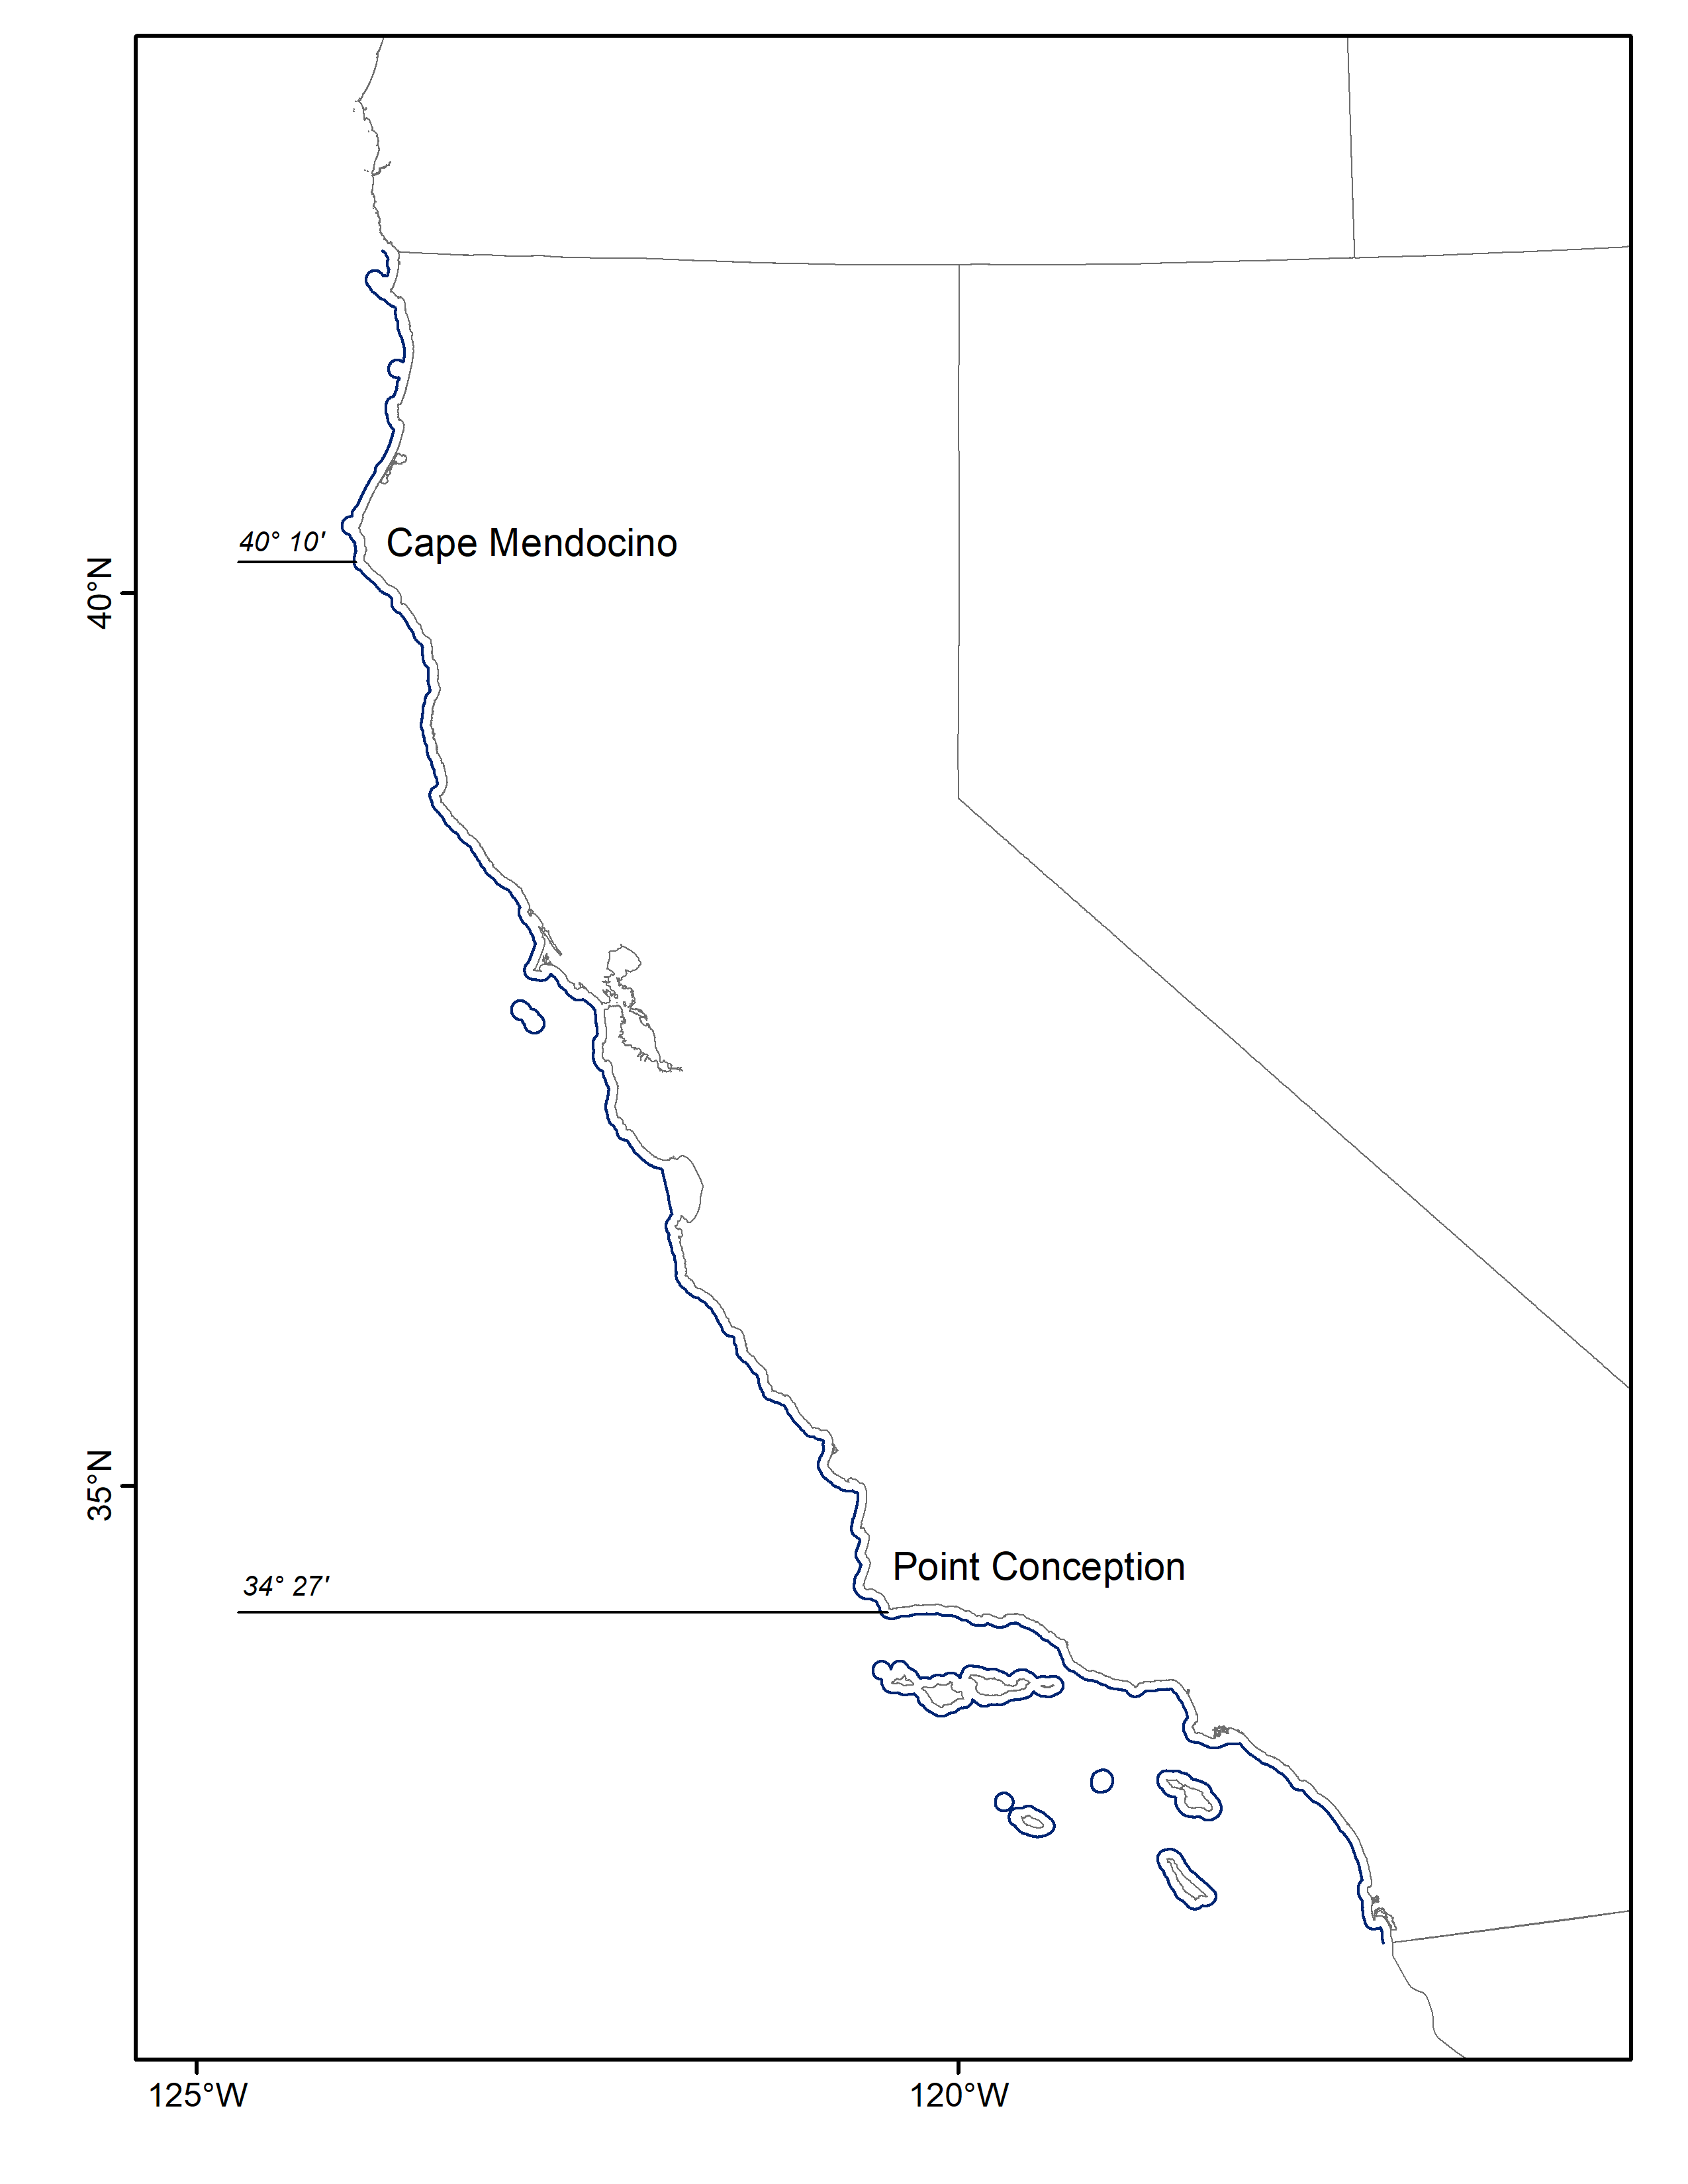
\includegraphics[width=1\textwidth,height=1\textheight]{C:/Stock_Assessments/VRML_Assessment_2021/GitHub/Vermilion_2021/doc/figures/assess_area.png}
\caption{Map of the assssment area with the 3 nm California stat water boundary. The northern California model includes areas from Pt. Conception to the California-Oregon border and the southern California assessment includes areas from Pt. Concpetion to the USA-Mexico border.\label{fig:assess-area}}
\end{figure}

\begin{figure}
\centering
\includegraphics[width=1\textwidth,height=1\textheight]{C:/Stock_Assessments/VRML_Assessment_2021/Model_files/SCA/Verm21SoCA_088_harms_survey_like_cowcod/plots/catch2 landings stacked.png}
\caption{Catches by fleet used in the base model.\label{fig:catch}}
\end{figure}

\begin{figure}
\centering
\includegraphics[width=0.5\textwidth,height=0.5\textheight]{C:/Stock_Assessments/VRML_Assessment_2021/Model_files/SCA/Verm21SoCA_088_harms_survey_like_cowcod/plots/comp_lendat_bubflt11mkt0.png}
\caption{Length composition data from the commercial hook-and-line fishery.\label{fig:len-data-COM-HKL}}
\end{figure}

\begin{figure}
\centering
\includegraphics[width=0.5\textwidth,height=0.5\textheight]{C:/Stock_Assessments/VRML_Assessment_2021/Model_files/SCA/Verm21SoCA_088_harms_survey_like_cowcod/plots/comp_lendat_data_weighting_TA1.8_COM_HKL.png}
\caption{Mean length for the commercial hook-and-line fishery with 95 percent confidence intervals.\label{fig:mean-com-len-data-COM-HKL}}
\end{figure}

\begin{figure}
\centering
\includegraphics[width=0.5\textwidth,height=0.5\textheight]{C:/Stock_Assessments/VRML_Assessment_2021/Model_files/SCA/Verm21SoCA_088_harms_survey_like_cowcod/plots/comp_lendat_bubflt3mkt0.png}
\caption{Length composition data from the commercial net fishery.\label{fig:len-data-COM-NET}}
\end{figure}

\begin{figure}
\centering
\includegraphics[width=0.5\textwidth,height=0.5\textheight]{C:/Stock_Assessments/VRML_Assessment_2021/Model_files/SCA/Verm21SoCA_088_harms_survey_like_cowcod/plots/comp_lendat_data_weighting_TA1.8_COM_NET.png}
\caption{Mean length for the commercial net fishery with 95 percent confidence intervals.\label{fig:mean-com-len-data-COM-NET}}
\end{figure}

\begin{figure}
\centering
\includegraphics[width=0.5\textwidth,height=0.5\textheight]{C:/Stock_Assessments/VRML_Assessment_2021/Model_files/SCA/Verm21SoCA_088_harms_survey_like_cowcod/plots/comp_lendat_bubflt4mkt0_page2.png}
\caption{Length composition data from the recreational PC retained fishery.\label{fig:len-data-REC-PC}}
\end{figure}

\begin{figure}
\centering
\includegraphics[width=0.5\textwidth,height=0.5\textheight]{C:/Stock_Assessments/VRML_Assessment_2021/Model_files/SCA/Verm21SoCA_088_harms_survey_like_cowcod/plots/comp_lendat_data_weighting_TA1.8_REC_PC.png}
\caption{Mean length for the recreational PC retained fishery with 95 percent confidence intervals.\label{fig:mean-com-len-data-REC-PC}}
\end{figure}

\begin{figure}
\centering
\includegraphics[width=0.5\textwidth,height=0.5\textheight]{C:/Stock_Assessments/VRML_Assessment_2021/Model_files/SCA/Verm21SoCA_088_harms_survey_like_cowcod/plots/comp_lendat_bubflt5mkt0.png}
\caption{Length composition data from the recreational PC discard fishery.\label{fig:len-data-REC-PC-DIS}}
\end{figure}

\begin{figure}
\centering
\includegraphics[width=0.5\textwidth,height=0.5\textheight]{C:/Stock_Assessments/VRML_Assessment_2021/Model_files/SCA/Verm21SoCA_088_harms_survey_like_cowcod/plots/comp_lendat_data_weighting_TA1.8_REC_PC_DIS.png}
\caption{Mean length for the recreational PC discard fishery with 95 percent confidence intervals.\label{fig:mean-com-len-data-REC-PC-DIS}}
\end{figure}

\begin{figure}
\centering
\includegraphics[width=0.5\textwidth,height=0.5\textheight]{C:/Stock_Assessments/VRML_Assessment_2021/Model_files/SCA/Verm21SoCA_088_harms_survey_like_cowcod/plots/comp_lendat_bubflt6mkt0_page2.png}
\caption{Length composition data from the recreational PR retained fishery.\label{fig:len-data-REC-PR}}
\end{figure}

\begin{figure}
\centering
\includegraphics[width=0.5\textwidth,height=0.5\textheight]{C:/Stock_Assessments/VRML_Assessment_2021/Model_files/SCA/Verm21SoCA_088_harms_survey_like_cowcod/plots/comp_lendat_data_weighting_TA1.8_REC_PR.png}
\caption{Mean length for the recreational PR retained fishery with 95 percent confidence intervals.\label{fig:mean-com-len-data-REC-PR}}
\end{figure}

\begin{figure}
\centering
\includegraphics[width=0.5\textwidth,height=0.5\textheight]{C:/Stock_Assessments/VRML_Assessment_2021/Model_files/SCA/Verm21SoCA_088_harms_survey_like_cowcod/plots/comp_lendat_bubflt8mkt0.png}
\caption{Length composition data from the NWFSC hook-and-line survey.\label{fig:len-data-NWFSC-HKL}}
\end{figure}

\begin{figure}
\centering
\includegraphics[width=0.5\textwidth,height=0.5\textheight]{C:/Stock_Assessments/VRML_Assessment_2021/Model_files/SCA/Verm21SoCA_088_harms_survey_like_cowcod/plots/comp_lendat_data_weighting_TA1.8_NWFSC_HKL.png}
\caption{Mean length for the NWFSC hook-and-line survey with 95 percent confidence intervals.\label{fig:mean-com-len-data-NWFSC-HKL}}
\end{figure}

\begin{figure}
\centering
\includegraphics[width=0.5\textwidth,height=0.5\textheight]{C:/Stock_Assessments/VRML_Assessment_2021/Model_files/SCA/Verm21SoCA_088_harms_survey_like_cowcod/plots/comp_lendat_bubflt9mkt0.png}
\caption{Length composition data from the West Coast Groundfish Bottomfish Trawl Survey.\label{fig:len-data-NWFSC-TWL}}
\end{figure}

\begin{figure}
\centering
\includegraphics[width=0.5\textwidth,height=0.5\textheight]{C:/Stock_Assessments/VRML_Assessment_2021/Model_files/SCA/Verm21SoCA_088_harms_survey_like_cowcod/plots/comp_lendat_data_weighting_TA1.8_NWFSC_TWL.png}
\caption{Mean length for the West Coast Groundfish Bottomfish Trawl Survey with 95 percent confidence intervals.\label{fig:mean-com-len-data-NWFSC-TWL}}
\end{figure}

\begin{figure}
\centering
\includegraphics[width=0.5\textwidth,height=0.5\textheight]{C:/Stock_Assessments/VRML_Assessment_2021/Model_files/SCA/Verm21SoCA_088_harms_survey_like_cowcod/plots/comp_lendat_bubflt11mkt0.png}
\caption{Length composition data from the CDFW reserach (aka green binder).\label{fig:len-data-CDFW-RESEARCH}}
\end{figure}

\begin{figure}
\centering
\includegraphics[width=0.5\textwidth,height=0.5\textheight]{C:/Stock_Assessments/VRML_Assessment_2021/Model_files/SCA/Verm21SoCA_088_harms_survey_like_cowcod/plots/comp_lendat_data_weighting_TA1.8_CDFW_RESEARCH.png}
\caption{Mean length for the CDFW reserach (aka green binder) with 95 percent confidence intervals.\label{fig:mean-com-len-data-CDFW-RESEARCH}}
\end{figure}

\begin{figure}
\centering
\includegraphics[width=0.5\textwidth,height=0.5\textheight]{C:/Stock_Assessments/VRML_Assessment_2021/Model_files/SCA/Verm21SoCA_088_harms_survey_like_cowcod/plots/comp_lendat_bubflt12mkt0.png}
\caption{Length composition data from the Dummy fleet.\label{fig:len-data-EARLY-HKL}}
\end{figure}

\begin{figure}
\centering
\includegraphics[width=0.5\textwidth,height=0.5\textheight]{C:/Stock_Assessments/VRML_Assessment_2021/Model_files/SCA/Verm21SoCA_088_harms_survey_like_cowcod/plots/comp_lendat_data_weighting_TA1.8_EARLY_HKL.png}
\caption{Mean length for the Dummy fleet with 95 percent confidence intervals.\label{fig:mean-com-len-data-EARLY-HKL}}
\end{figure}

\begin{figure}
\centering
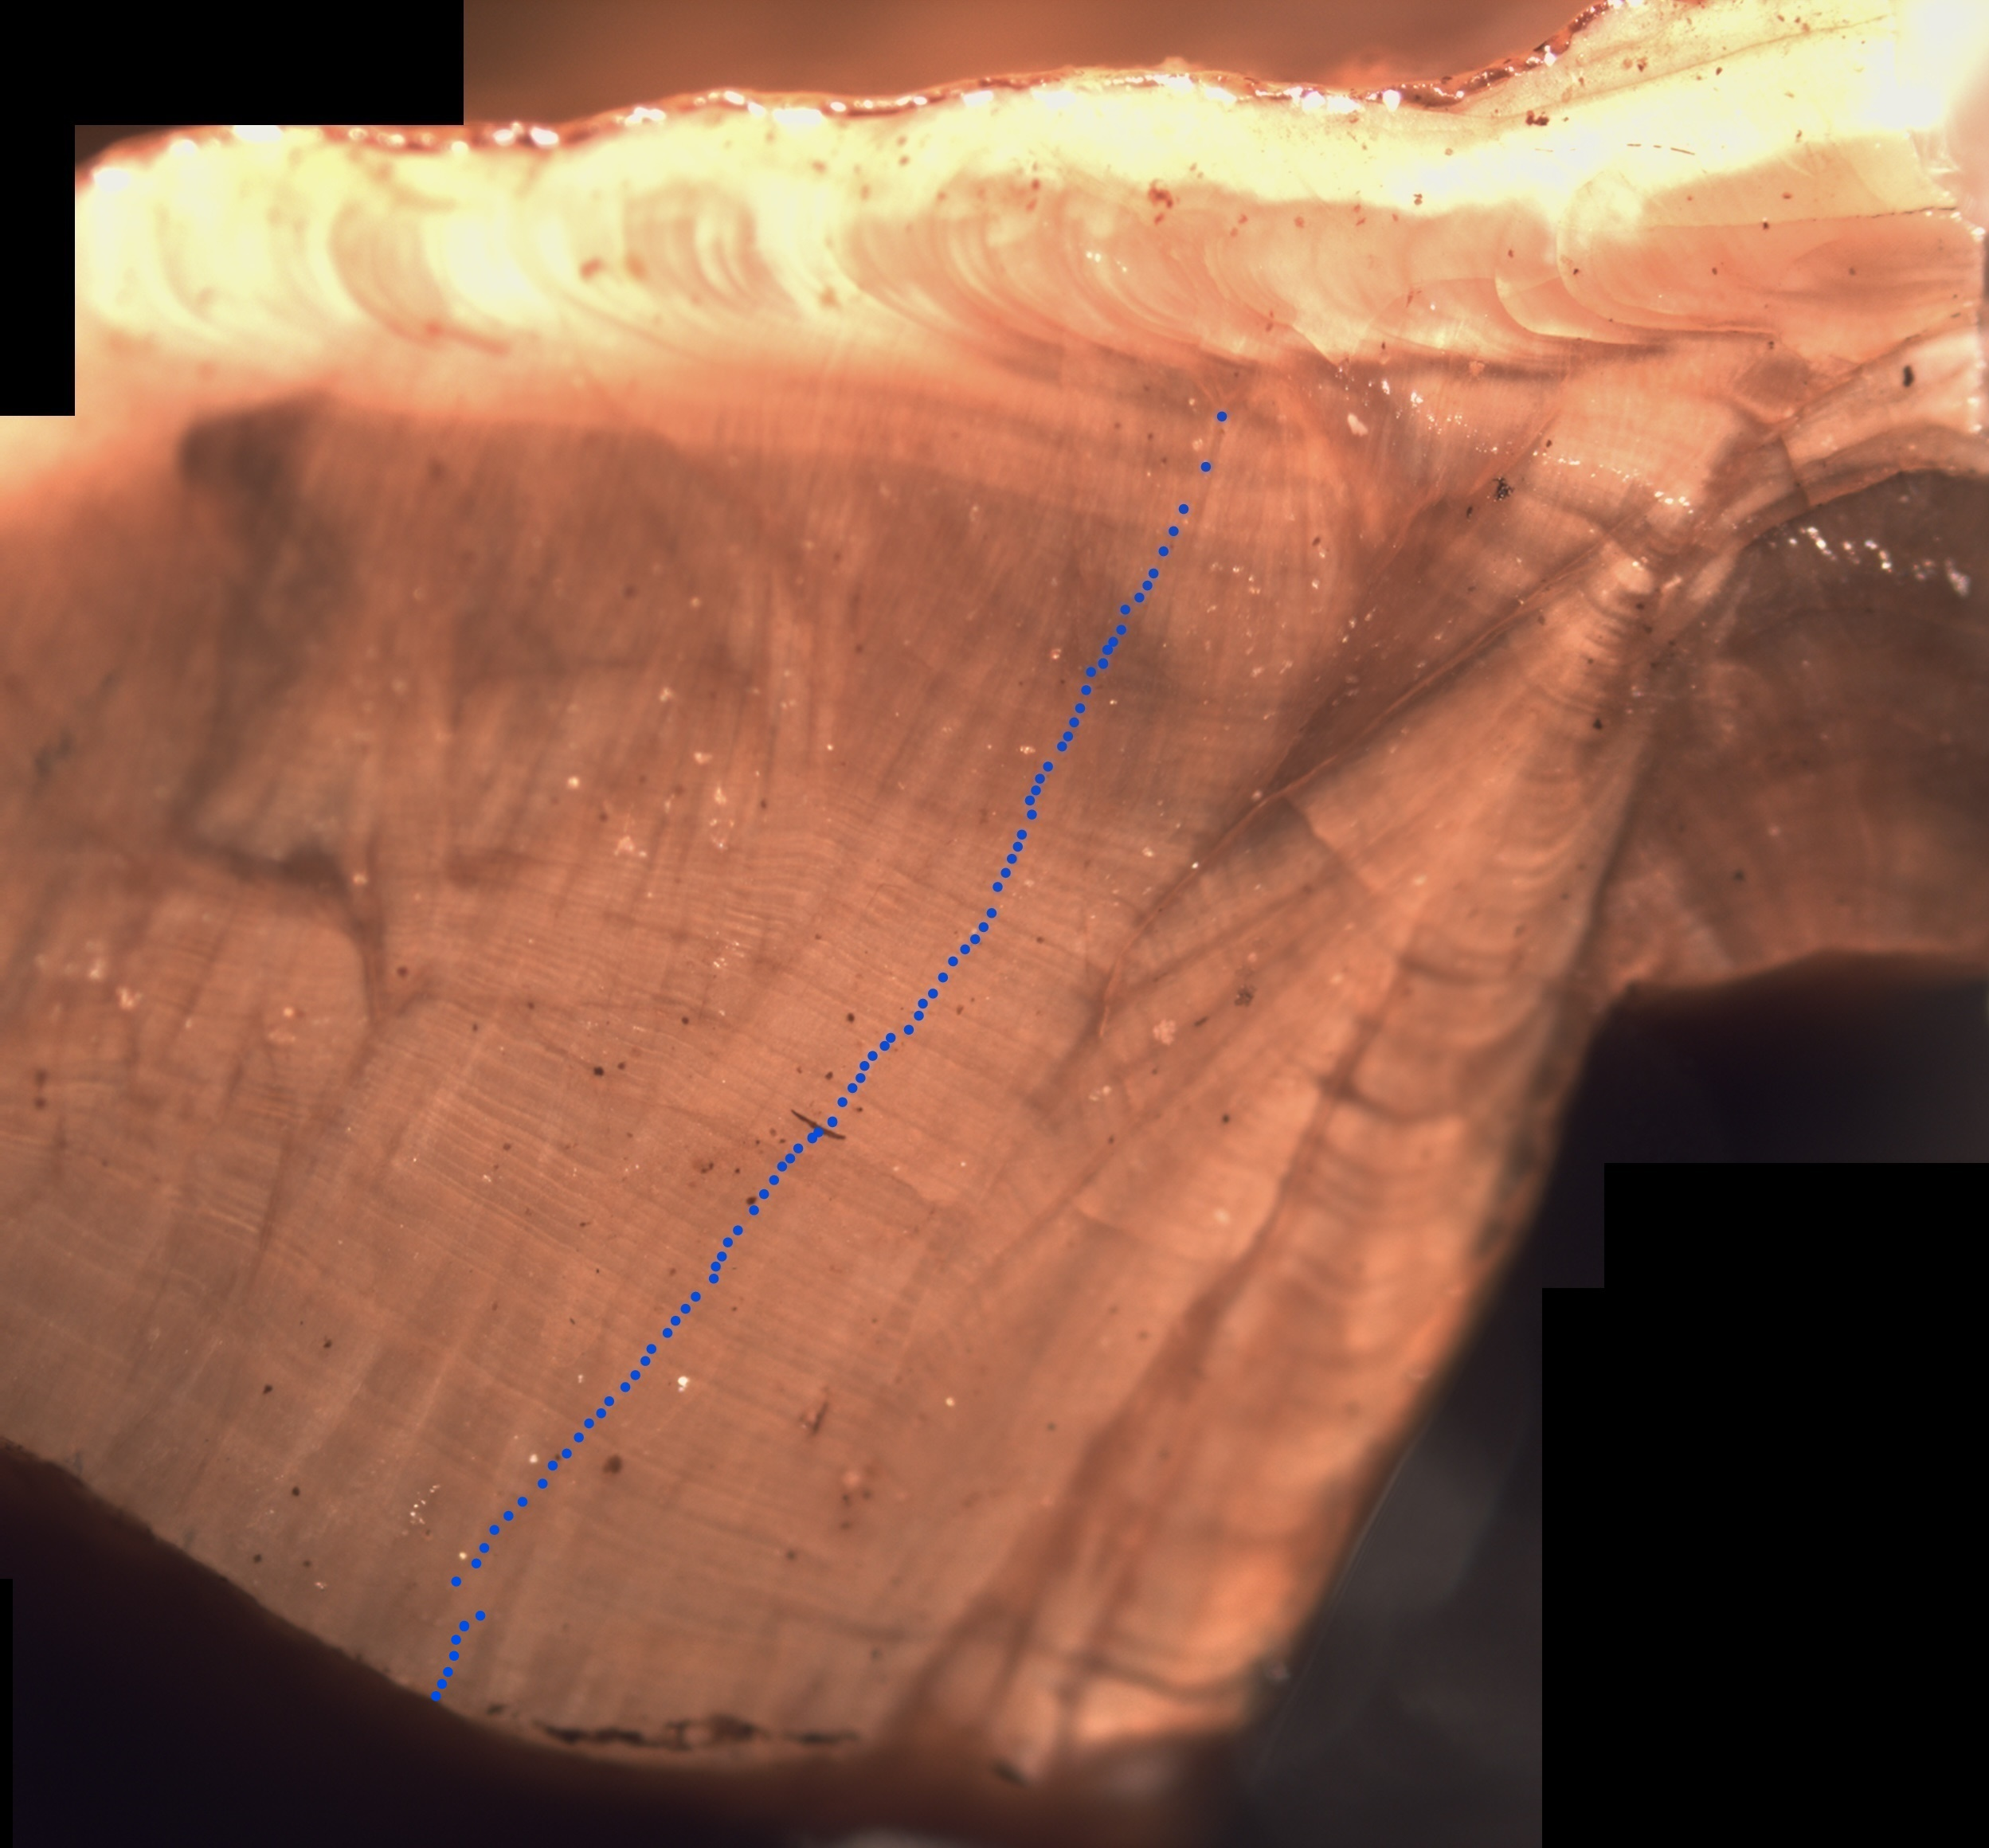
\includegraphics[width=1\textwidth,height=1\textheight]{C:/Stock_Assessments/VRML_Assessment_2021/GitHub/Vermilion_2021/doc/figures/oldfish.jpg}
\caption{Photograph of the \emph{oldest} aged fish used in the assessment with annuli marked by B. Kamikawa (NWFSC)..\label{fig:oldfish}}
\end{figure}

\begin{figure}
\centering
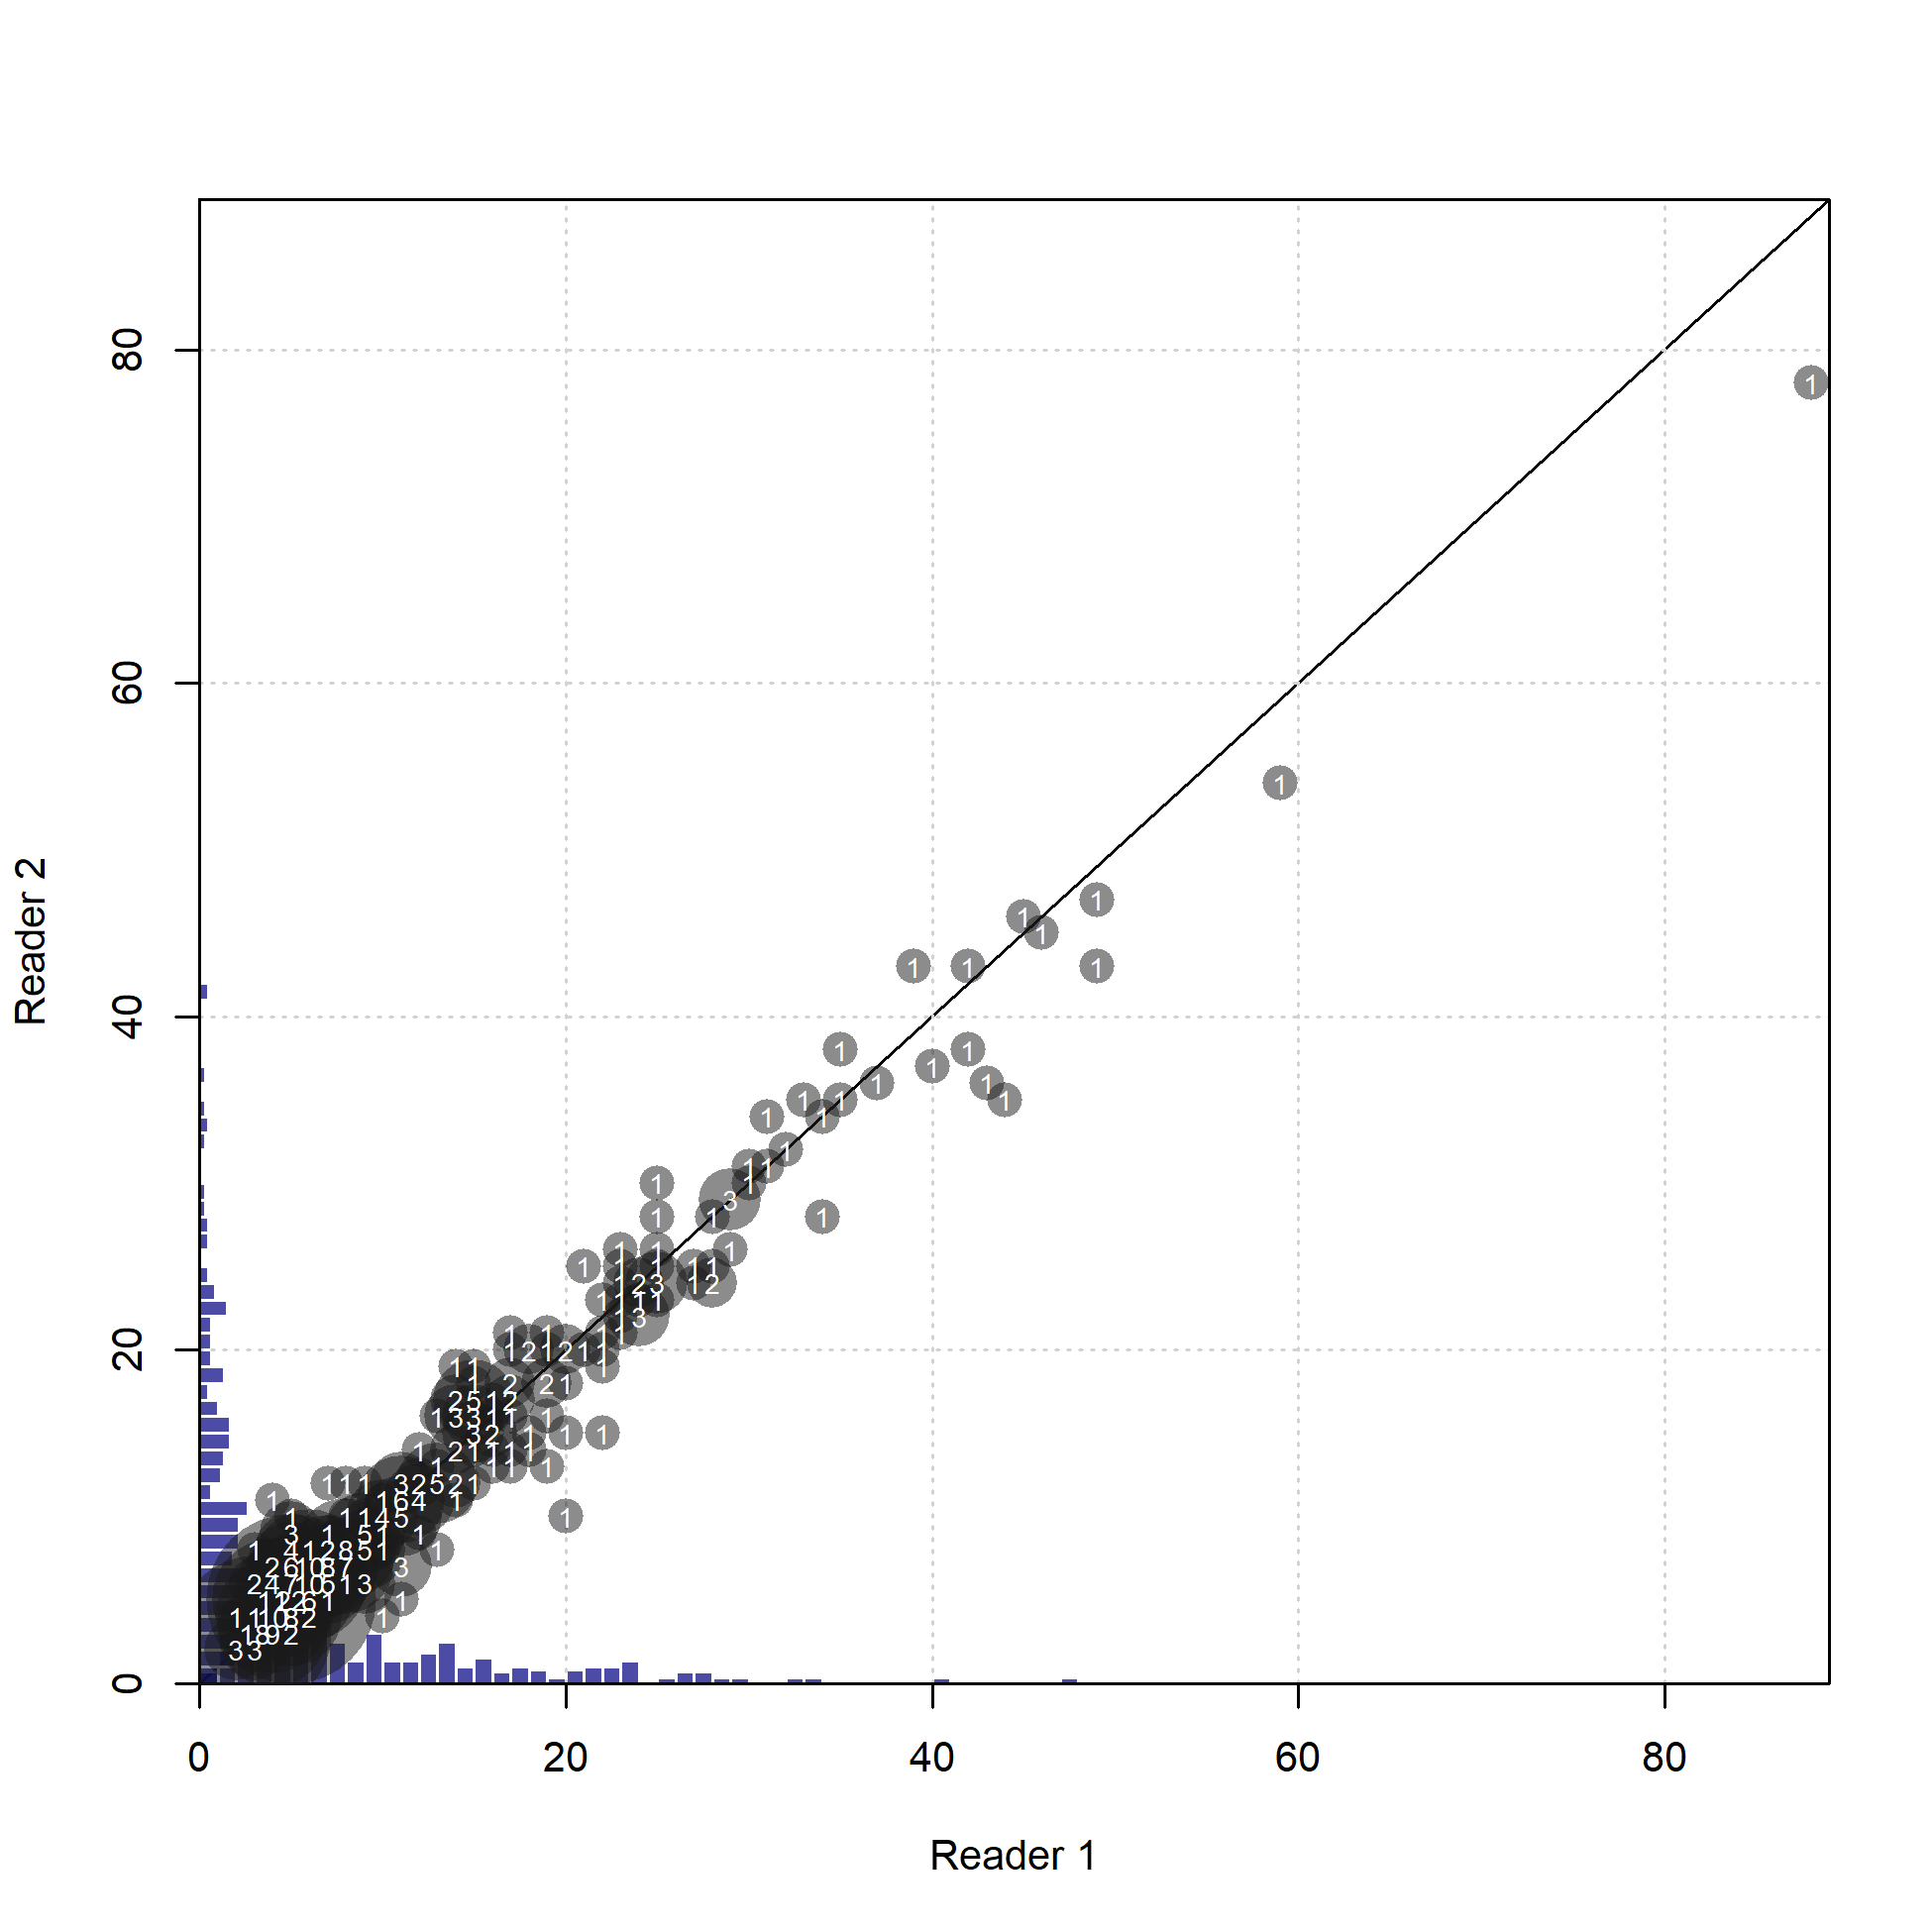
\includegraphics[width=1\textwidth,height=1\textheight]{C:/Stock_Assessments/VRML_Assessment_2021/GitHub/Vermilion_2021/doc/figures/Reader 1 vs Reader 2.png}
\caption{Aging precision between initial and blind double reads for vermilion. Numbers in the bubbles are the sample sizes of otoliths cross-read..\label{fig:reader1reader2}}
\end{figure}

\begin{figure}
\centering
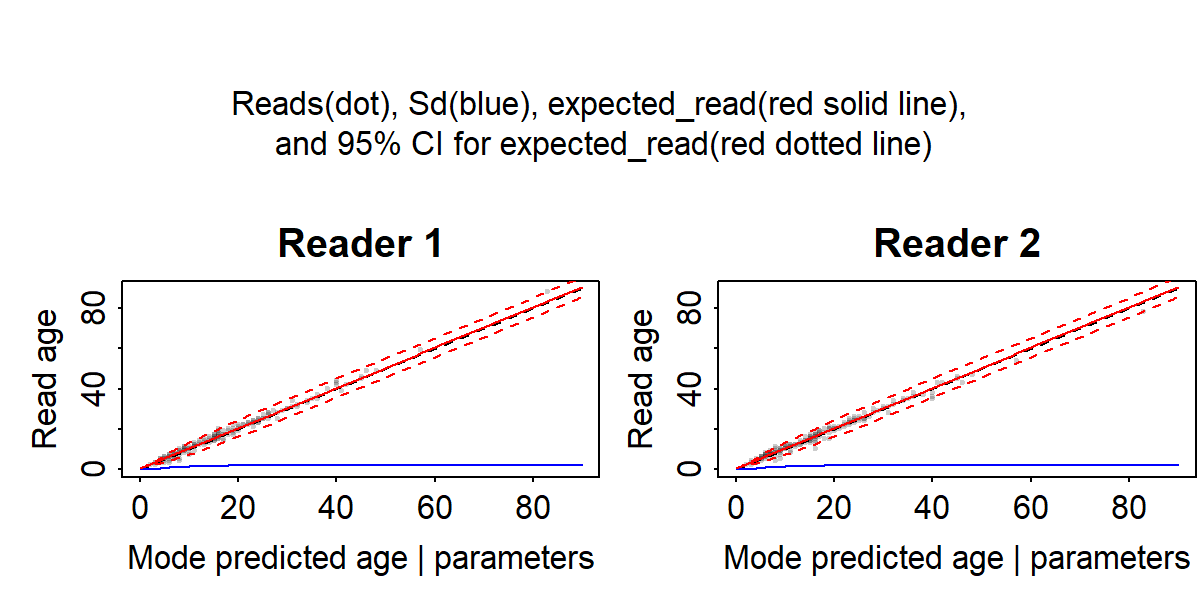
\includegraphics[width=1\textwidth,height=1\textheight]{C:/Stock_Assessments/VRML_Assessment_2021/GitHub/Vermilion_2021/doc/figures/True vs Reads (by reader).png}
\caption{True versus predicted age for two current age readers at the NWFSC from the ageing error software with unbiased reads for reader 1 and curvilinear bias for reader 1 and curvilinear standard deviation for both readers..\label{fig:truereads}}
\end{figure}

\begin{figure}
\centering
\includegraphics[width=1\textwidth,height=1\textheight]{C:/Stock_Assessments/VRML_Assessment_2021/Model_files/SCA/Verm21SoCA_088_harms_survey_like_cowcod/plots/numbers10_ageerror_matrix_1.png}
\caption{Distribution of observed age at true age for ageing error type 1.\label{fig:ageerror}}
\end{figure}

\begin{figure}
\centering
\includegraphics[width=1\textwidth,height=1\textheight]{C:/Stock_Assessments/VRML_Assessment_2021/Model_files/SCA/Verm21SoCA_088_harms_survey_like_cowcod/plots/bio1_sizeatage.png}
\caption{Length at age in the beginning of the year (or season) in the ending year of the model. Shaded area indicates 95\% distribution of length at age around estimated growth curve.\label{fig:fittedgrowth}}
\end{figure}

\begin{figure}
\centering
\includegraphics[width=1\textwidth,height=1\textheight]{C:/Stock_Assessments/VRML_Assessment_2021/Model_files/SCA/Verm21SoCA_088_harms_survey_like_cowcod/plots/bio5_weightatsize.png}
\caption{Weight-length relationship.\label{fig:weightlength}}
\end{figure}

\begin{figure}
\centering
\includegraphics[width=1\textwidth,height=1\textheight]{C:/Stock_Assessments/VRML_Assessment_2021/Model_files/SCA/Verm21SoCA_088_harms_survey_like_cowcod/plots/bio6_maturity.png}
\caption{Maturity at length.\label{fig:maturity}}
\end{figure}

\begin{figure}
\centering
\includegraphics[width=1\textwidth,height=1\textheight]{C:/Stock_Assessments/VRML_Assessment_2021/Model_files/SCA/Verm21SoCA_088_harms_survey_like_cowcod/plots/bio8_fecundity_wt.png}
\caption{Fecundity as a function of weight.\label{fig:fecundity}}
\end{figure}

\begin{figure}
\centering
\includegraphics[width=1\textwidth,height=1\textheight]{C:/Stock_Assessments/VRML_Assessment_2021/Model_files/SCA/Verm21SoCA_088_harms_survey_like_cowcod/plots/bio11_spawningoutput_age.png}
\caption{Spawning output at age. This is the product of maturity and fecundity. When these processes are length-based they are converted into the age dimension using the matrix of length at age.\label{fig:spawningoutputage}}
\end{figure}

\FloatBarrier

\FloatBarrier

\begin{figure}
\centering
\includegraphics[width=1\textwidth,height=1\textheight]{C:/Stock_Assessments/VRML_Assessment_2021/Model_files/SCA/Verm21SoCA_088_harms_survey_like_cowcod/plots/sel01_multiple_fleets_length1.png}
\caption{Selectivity at length by fleet.\label{fig:selex-length-all}}
\end{figure}

\FloatBarrier

\begin{figure}
\centering
\includegraphics[width=1\textwidth,height=1\textheight]{C:/Stock_Assessments/VRML_Assessment_2021/Model_files/SCA/Verm21SoCA_088_harms_survey_like_cowcod/plots/sel02_multiple_fleets_age1.png}
\caption{Selectivity at age derived from selectivity at length for multiple fleets.\label{fig:selex-age-all}}
\end{figure}

\begin{figure}
\centering
\includegraphics[width=1\textwidth,height=1\textheight]{C:/Stock_Assessments/VRML_Assessment_2021/Model_files/SCA/Verm21SoCA_088_harms_survey_like_cowcod/plots/sel03_len_timevary_surf_flt1sex1.png}
\caption{Surface plot of Female time-varying selectivity for COM\_HKL.\label{fig:sel03_len_timevary_surf_flt1sex1}}
\end{figure}

\begin{figure}
\centering
\includegraphics[width=1\textwidth,height=1\textheight]{C:/Stock_Assessments/VRML_Assessment_2021/Model_files/SCA/Verm21SoCA_088_harms_survey_like_cowcod/plots/sel03_len_timevary_surf_flt2sex1.png}
\caption{Surface plot of Female time-varying selectivity for COM\_TWL.\label{fig:sel03_len_timevary_surf_flt2sex1}}
\end{figure}

\begin{figure}
\centering
\includegraphics[width=1\textwidth,height=1\textheight]{C:/Stock_Assessments/VRML_Assessment_2021/Model_files/SCA/Verm21SoCA_088_harms_survey_like_cowcod/plots/sel03_len_timevary_surf_flt4sex1.png}
\caption{Surface plot of Female time-varying selectivity for REC\_PC.\label{fig:sel03_len_timevary_surf_flt4sex1}}
\end{figure}

\begin{figure}
\centering
\includegraphics[width=1\textwidth,height=1\textheight]{C:/Stock_Assessments/VRML_Assessment_2021/Model_files/SCA/Verm21SoCA_088_harms_survey_like_cowcod/plots/sel03_len_timevary_surf_flt6sex1.png}
\caption{Surface plot of Female time-varying selectivity for REC\_PR.\label{fig:sel03_len_timevary_surf_flt6sex1}}
\end{figure}

\begin{figure}
\centering
\includegraphics[width=1\textwidth,height=1\textheight]{C:/Stock_Assessments/VRML_Assessment_2021/Model_files/SCA/Verm21SoCA_088_harms_survey_like_cowcod/plots/sel03_len_timevary_surf_flt10sex1.png}
\caption{Surface plot of Female time-varying selectivity for REC\_PC\_ONBOARD.\label{fig:sel03_len_timevary_surf_flt10sex1}}
\end{figure}

\FloatBarrier

\FloatBarrier

\begin{figure}
\centering
\includegraphics[width=0.5\textwidth,height=0.5\textheight]{C:/Stock_Assessments/VRML_Assessment_2021/Model_files/SCA/Verm21SoCA_088_harms_survey_like_cowcod/plots/sel09_len_flt1sex1.png}
\caption{Female ending year selectivity for the commercial hook-and-line fishery.\label{fig:endyr-selex-COM-HKL}}
\end{figure}

\begin{figure}
\centering
\includegraphics[width=0.5\textwidth,height=0.5\textheight]{C:/Stock_Assessments/VRML_Assessment_2021/Model_files/SCA/Verm21SoCA_088_harms_survey_like_cowcod/plots/sel09_len_flt3sex1.png}
\caption{Female ending year selectivity for the commercial net fishery.\label{fig:endyr-selex-COM-NET}}
\end{figure}

\begin{figure}
\centering
\includegraphics[width=0.5\textwidth,height=0.5\textheight]{C:/Stock_Assessments/VRML_Assessment_2021/Model_files/SCA/Verm21SoCA_088_harms_survey_like_cowcod/plots/sel09_len_flt4sex1.png}
\caption{Female ending year selectivity for the recreational PC retained fishery.\label{fig:endyr-selex-REC-PC}}
\end{figure}

\begin{figure}
\centering
\includegraphics[width=0.5\textwidth,height=0.5\textheight]{C:/Stock_Assessments/VRML_Assessment_2021/Model_files/SCA/Verm21SoCA_088_harms_survey_like_cowcod/plots/sel09_len_flt5sex1.png}
\caption{Female ending year selectivity for the recreational PC discard fishery.\label{fig:endyr-selex-REC-PC-DIS}}
\end{figure}

\begin{figure}
\centering
\includegraphics[width=0.5\textwidth,height=0.5\textheight]{C:/Stock_Assessments/VRML_Assessment_2021/Model_files/SCA/Verm21SoCA_088_harms_survey_like_cowcod/plots/sel09_len_flt6sex1.png}
\caption{Female ending year selectivity for the recreational PR retained fishery.\label{fig:endyr-selex-REC-PR}}
\end{figure}

\begin{figure}
\centering
\includegraphics[width=0.5\textwidth,height=0.5\textheight]{C:/Stock_Assessments/VRML_Assessment_2021/Model_files/SCA/Verm21SoCA_088_harms_survey_like_cowcod/plots/sel09_len_flt8sex1.png}
\caption{Female ending year selectivity for the NWFSC hook-and-line survey.\label{fig:endyr-selex-NWFSC-HKL}}
\end{figure}

\begin{figure}
\centering
\includegraphics[width=0.5\textwidth,height=0.5\textheight]{C:/Stock_Assessments/VRML_Assessment_2021/Model_files/SCA/Verm21SoCA_088_harms_survey_like_cowcod/plots/sel09_len_flt9sex1.png}
\caption{Female ending year selectivity for the West Coast Groundfish Bottomfish Trawl Survey.\label{fig:endyr-selex-NWFSC-TWL}}
\end{figure}

\begin{figure}
\centering
\includegraphics[width=0.5\textwidth,height=0.5\textheight]{C:/Stock_Assessments/VRML_Assessment_2021/Model_files/SCA/Verm21SoCA_088_harms_survey_like_cowcod/plots/sel09_len_flt2sex1.png}
\caption{Female ending year selectivity for the commercial trawl fishery.\label{fig:endyr-selex-COM-TWL}}
\end{figure}

\begin{figure}
\centering
\includegraphics[width=0.5\textwidth,height=0.5\textheight]{C:/Stock_Assessments/VRML_Assessment_2021/Model_files/SCA/Verm21SoCA_088_harms_survey_like_cowcod/plots/sel09_len_flt7sex1.png}
\caption{Female ending year selectivity for the recreational PR discard fishery.\label{fig:endyr-selex-REC-PR-DIS}}
\end{figure}

\FloatBarrier

\FloatBarrier

\begin{figure}
\centering
\includegraphics[width=1\textwidth,height=1\textheight]{C:/Stock_Assessments/VRML_Assessment_2021/Model_files/SCA/Verm21SoCA_088_harms_survey_like_cowcod/plots/comp_lenfit__aggregated_across_time.png}
\caption{Length comps, aggregated across time by fleet. Labels `retained' and `discard' indicate discarded or retained sampled for each fleet. Panels without this designation represent the whole catch.\label{fig:lenfits-all}}
\end{figure}

\begin{figure}
\centering
\includegraphics[width=0.5\textwidth,height=0.5\textheight]{C:/Stock_Assessments/VRML_Assessment_2021/Model_files/SCA/Verm21SoCA_088_harms_survey_like_cowcod/plots/comp_lenfit_residsflt11mkt0.png}
\caption{Pearson residuals for the commercial hook-and-line fishery. Closed bubbles are positive residuals (observed \textgreater{} expected) and open bubbles are negative residuals (observed \textless{} expected).\label{fig:len-pearson-COM-HKL}}
\end{figure}

\begin{figure}
\centering
\includegraphics[width=0.5\textwidth,height=0.5\textheight]{C:/Stock_Assessments/VRML_Assessment_2021/Model_files/SCA/Verm21SoCA_088_harms_survey_like_cowcod/plots/comp_lenfit_data_weighting_TA1.8_COM_HKL.png}
\caption{Mean length for REC\_PR with 95\% confidence intervals based on current samples sizes. Francis data weighting method TA1.8: thinner intervals (with capped ends) show result of further adjusting sample sizes based on suggested multiplier (with 95\% interval) for length data from the commercial hook-and-line fishery.\label{fig:mean-len-fit-COM-HKL}}
\end{figure}

\begin{figure}
\centering
\includegraphics[width=0.5\textwidth,height=0.5\textheight]{C:/Stock_Assessments/VRML_Assessment_2021/Model_files/SCA/Verm21SoCA_088_harms_survey_like_cowcod/plots/comp_lenfit_residsflt3mkt0.png}
\caption{Pearson residuals for the commercial net fishery. Closed bubbles are positive residuals (observed \textgreater{} expected) and open bubbles are negative residuals (observed \textless{} expected).\label{fig:len-pearson-COM-NET}}
\end{figure}

\begin{figure}
\centering
\includegraphics[width=0.5\textwidth,height=0.5\textheight]{C:/Stock_Assessments/VRML_Assessment_2021/Model_files/SCA/Verm21SoCA_088_harms_survey_like_cowcod/plots/comp_lenfit_data_weighting_TA1.8_COM_NET.png}
\caption{Mean length for REC\_PR with 95\% confidence intervals based on current samples sizes. Francis data weighting method TA1.8: thinner intervals (with capped ends) show result of further adjusting sample sizes based on suggested multiplier (with 95\% interval) for length data from the commercial net fishery.\label{fig:mean-len-fit-COM-NET}}
\end{figure}

\begin{figure}
\centering
\includegraphics[width=0.5\textwidth,height=0.5\textheight]{C:/Stock_Assessments/VRML_Assessment_2021/Model_files/SCA/Verm21SoCA_088_harms_survey_like_cowcod/plots/comp_lenfit_residsflt4mkt0_page2.png}
\caption{Pearson residuals for the recreational PC retained fishery. Closed bubbles are positive residuals (observed \textgreater{} expected) and open bubbles are negative residuals (observed \textless{} expected).\label{fig:len-pearson-REC-PC}}
\end{figure}

\begin{figure}
\centering
\includegraphics[width=0.5\textwidth,height=0.5\textheight]{C:/Stock_Assessments/VRML_Assessment_2021/Model_files/SCA/Verm21SoCA_088_harms_survey_like_cowcod/plots/comp_lenfit_data_weighting_TA1.8_REC_PC.png}
\caption{Mean length for REC\_PR with 95\% confidence intervals based on current samples sizes. Francis data weighting method TA1.8: thinner intervals (with capped ends) show result of further adjusting sample sizes based on suggested multiplier (with 95\% interval) for length data from the recreational PC retained fishery.\label{fig:mean-len-fit-REC-PC}}
\end{figure}

\begin{figure}
\centering
\includegraphics[width=0.5\textwidth,height=0.5\textheight]{C:/Stock_Assessments/VRML_Assessment_2021/Model_files/SCA/Verm21SoCA_088_harms_survey_like_cowcod/plots/comp_lenfit_residsflt5mkt0.png}
\caption{Pearson residuals for the recreational PC discard fishery. Closed bubbles are positive residuals (observed \textgreater{} expected) and open bubbles are negative residuals (observed \textless{} expected).\label{fig:len-pearson-REC-PC-DIS}}
\end{figure}

\begin{figure}
\centering
\includegraphics[width=0.5\textwidth,height=0.5\textheight]{C:/Stock_Assessments/VRML_Assessment_2021/Model_files/SCA/Verm21SoCA_088_harms_survey_like_cowcod/plots/comp_lenfit_data_weighting_TA1.8_REC_PC_DIS.png}
\caption{Mean length for REC\_PR with 95\% confidence intervals based on current samples sizes. Francis data weighting method TA1.8: thinner intervals (with capped ends) show result of further adjusting sample sizes based on suggested multiplier (with 95\% interval) for length data from the recreational PC discard fishery.\label{fig:mean-len-fit-REC-PC-DIS}}
\end{figure}

\begin{figure}
\centering
\includegraphics[width=0.5\textwidth,height=0.5\textheight]{C:/Stock_Assessments/VRML_Assessment_2021/Model_files/SCA/Verm21SoCA_088_harms_survey_like_cowcod/plots/comp_lenfit_residsflt6mkt0_page2.png}
\caption{Pearson residuals for the recreational PR retained fishery. Closed bubbles are positive residuals (observed \textgreater{} expected) and open bubbles are negative residuals (observed \textless{} expected).\label{fig:len-pearson-REC-PR}}
\end{figure}

\begin{figure}
\centering
\includegraphics[width=0.5\textwidth,height=0.5\textheight]{C:/Stock_Assessments/VRML_Assessment_2021/Model_files/SCA/Verm21SoCA_088_harms_survey_like_cowcod/plots/comp_lenfit_data_weighting_TA1.8_REC_PR.png}
\caption{Mean length for REC\_PR with 95\% confidence intervals based on current samples sizes. Francis data weighting method TA1.8: thinner intervals (with capped ends) show result of further adjusting sample sizes based on suggested multiplier (with 95\% interval) for length data from the recreational PR retained fishery.\label{fig:mean-len-fit-REC-PR}}
\end{figure}

\begin{figure}
\centering
\includegraphics[width=0.5\textwidth,height=0.5\textheight]{C:/Stock_Assessments/VRML_Assessment_2021/Model_files/SCA/Verm21SoCA_088_harms_survey_like_cowcod/plots/comp_lenfit_residsflt8mkt0.png}
\caption{Pearson residuals for the NWFSC hook-and-line survey. Closed bubbles are positive residuals (observed \textgreater{} expected) and open bubbles are negative residuals (observed \textless{} expected).\label{fig:len-pearson-NWFSC-HKL}}
\end{figure}

\begin{figure}
\centering
\includegraphics[width=0.5\textwidth,height=0.5\textheight]{C:/Stock_Assessments/VRML_Assessment_2021/Model_files/SCA/Verm21SoCA_088_harms_survey_like_cowcod/plots/comp_lenfit_data_weighting_TA1.8_NWFSC_HKL.png}
\caption{Mean length for REC\_PR with 95\% confidence intervals based on current samples sizes. Francis data weighting method TA1.8: thinner intervals (with capped ends) show result of further adjusting sample sizes based on suggested multiplier (with 95\% interval) for length data from the NWFSC hook-and-line survey.\label{fig:mean-len-fit-NWFSC-HKL}}
\end{figure}

\begin{figure}
\centering
\includegraphics[width=0.5\textwidth,height=0.5\textheight]{C:/Stock_Assessments/VRML_Assessment_2021/Model_files/SCA/Verm21SoCA_088_harms_survey_like_cowcod/plots/comp_lenfit_residsflt9mkt0.png}
\caption{Pearson residuals for the West Coast Groundfish Bottomfish Trawl Survey. Closed bubbles are positive residuals (observed \textgreater{} expected) and open bubbles are negative residuals (observed \textless{} expected).\label{fig:len-pearson-NWFSC-TWL}}
\end{figure}

\begin{figure}
\centering
\includegraphics[width=0.5\textwidth,height=0.5\textheight]{C:/Stock_Assessments/VRML_Assessment_2021/Model_files/SCA/Verm21SoCA_088_harms_survey_like_cowcod/plots/comp_lenfit_data_weighting_TA1.8_NWFSC_TWL.png}
\caption{Mean length for REC\_PR with 95\% confidence intervals based on current samples sizes. Francis data weighting method TA1.8: thinner intervals (with capped ends) show result of further adjusting sample sizes based on suggested multiplier (with 95\% interval) for length data from the West Coast Groundfish Bottomfish Trawl Survey.\label{fig:mean-len-fit-NWFSC-TWL}}
\end{figure}

\begin{figure}
\centering
\includegraphics[width=0.5\textwidth,height=0.5\textheight]{C:/Stock_Assessments/VRML_Assessment_2021/Model_files/SCA/Verm21SoCA_088_harms_survey_like_cowcod/plots/comp_lenfit_residsflt11mkt0.png}
\caption{Pearson residuals for the CDFW reserach (aka green binder). Closed bubbles are positive residuals (observed \textgreater{} expected) and open bubbles are negative residuals (observed \textless{} expected).\label{fig:len-pearson-CDFW-RESEARCH}}
\end{figure}

\begin{figure}
\centering
\includegraphics[width=0.5\textwidth,height=0.5\textheight]{C:/Stock_Assessments/VRML_Assessment_2021/Model_files/SCA/Verm21SoCA_088_harms_survey_like_cowcod/plots/comp_lenfit_data_weighting_TA1.8_CDFW_RESEARCH.png}
\caption{Mean length for REC\_PR with 95\% confidence intervals based on current samples sizes. Francis data weighting method TA1.8: thinner intervals (with capped ends) show result of further adjusting sample sizes based on suggested multiplier (with 95\% interval) for length data from the CDFW reserach (aka green binder).\label{fig:mean-len-fit-CDFW-RESEARCH}}
\end{figure}

\begin{figure}
\centering
\includegraphics[width=0.5\textwidth,height=0.5\textheight]{C:/Stock_Assessments/VRML_Assessment_2021/Model_files/SCA/Verm21SoCA_088_harms_survey_like_cowcod/plots/comp_lenfit_residsflt12mkt0.png}
\caption{Pearson residuals for the Dummy fleet. Closed bubbles are positive residuals (observed \textgreater{} expected) and open bubbles are negative residuals (observed \textless{} expected).\label{fig:len-pearson-EARLY-HKL}}
\end{figure}

\begin{figure}
\centering
\includegraphics[width=0.5\textwidth,height=0.5\textheight]{C:/Stock_Assessments/VRML_Assessment_2021/Model_files/SCA/Verm21SoCA_088_harms_survey_like_cowcod/plots/comp_lenfit_data_weighting_TA1.8_EARLY_HKL.png}
\caption{Mean length for REC\_PR with 95\% confidence intervals based on current samples sizes. Francis data weighting method TA1.8: thinner intervals (with capped ends) show result of further adjusting sample sizes based on suggested multiplier (with 95\% interval) for length data from the Dummy fleet.\label{fig:mean-len-fit-EARLY-HKL}}
\end{figure}

\begin{figure}
\centering
\includegraphics[width=0.5\textwidth,height=0.5\textheight]{C:/Stock_Assessments/VRML_Assessment_2021/Model_files/SCA/Verm21SoCA_088_harms_survey_like_cowcod/plots/sexratio_len_flt11mkt0.png}
\caption{Sex ratios for length comps, whole catchCDFW reserach (aka green binder). Observed sex ratios (points) with 75\% intervals (vertical lines) calculated as a Jeffreys interval based on the adjusted input sample size. The model expectation is shown in the purple line.\label{fig:sexratio-CDFW-RESEARCH}}
\end{figure}

\begin{figure}
\centering
\includegraphics[width=0.5\textwidth,height=0.5\textheight]{C:/Stock_Assessments/VRML_Assessment_2021/Model_files/SCA/Verm21SoCA_088_harms_survey_like_cowcod/plots/sexratio_len_flt12mkt0.png}
\caption{Sex ratios for length comps, whole catchDummy fleet. Observed sex ratios (points) with 75\% intervals (vertical lines) calculated as a Jeffreys interval based on the adjusted input sample size. The model expectation is shown in the purple line.\label{fig:sexratio-EARLY-HKL}}
\end{figure}

\begin{figure}
\centering
\includegraphics[width=0.5\textwidth,height=0.5\textheight]{C:/Stock_Assessments/VRML_Assessment_2021/Model_files/SCA/Verm21SoCA_088_harms_survey_like_cowcod/plots/sexratio_len_flt8mkt0.png}
\caption{Sex ratios for length comps, whole catchNWFSC hook-and-line survey. Observed sex ratios (points) with 75\% intervals (vertical lines) calculated as a Jeffreys interval based on the adjusted input sample size. The model expectation is shown in the purple line.\label{fig:sexratio-NWFSC-HKL}}
\end{figure}

\begin{figure}
\centering
\includegraphics[width=0.5\textwidth,height=0.5\textheight]{C:/Stock_Assessments/VRML_Assessment_2021/Model_files/SCA/Verm21SoCA_088_harms_survey_like_cowcod/plots/sexratio_len_flt9mkt0.png}
\caption{Sex ratios for length comps, whole catchWest Coast Groundfish Bottomfish Trawl Survey. Observed sex ratios (points) with 75\% intervals (vertical lines) calculated as a Jeffreys interval based on the adjusted input sample size. The model expectation is shown in the purple line.\label{fig:sexratio-NWFSC-TWL}}
\end{figure}

\FloatBarrier

\begin{figure}
\centering
\includegraphics[width=1\textwidth,height=1\textheight]{C:/Stock_Assessments/VRML_Assessment_2021/Model_files/SCA/Verm21SoCA_088_harms_survey_like_cowcod/plots/ts7_Spawning_output_with_95_asymptotic_intervals_intervals.png}
\caption{Estimated time series of spawning output.\label{fig:ssb}}
\end{figure}

\begin{figure}
\centering
\includegraphics[width=1\textwidth,height=1\textheight]{C:/Stock_Assessments/VRML_Assessment_2021/Model_files/SCA/Verm21SoCA_088_harms_survey_like_cowcod/plots/ts9_Relative_spawning_output_intervals.png}
\caption{Estimated time series of relative spawning output.\label{fig:depl}}
\end{figure}

\FloatBarrier

\begin{figure}
\centering
\includegraphics[width=0.5\textwidth,height=0.5\textheight]{C:/Stock_Assessments/VRML_Assessment_2021/Model_files/SCA/Verm21SoCA_088_harms_survey_like_cowcod/plots/index9_standcpueall.png}
\caption{Standardized indices overlaid. Each index is rescaled to have mean observation = 1.0.\label{fig:cpueall}}
\end{figure}

\begin{figure}
\centering
\includegraphics[width=0.5\textwidth,height=0.5\textheight]{C:/Stock_Assessments/VRML_Assessment_2021/Model_files/SCA/Verm21SoCA_088_harms_survey_like_cowcod/plots/index5_logcpuefit_REC_PC.png}
\caption{Fit to log index data on log scale for the recreational PC retained fishery. Lines indicate 95\% uncertainty interval around index values based on the model assumption of lognormal error. Thicker lines (if present) indicate input uncertainty before addition of estimated additional uncertainty parameter.\label{fig:log-cpue-REC-PC}}
\end{figure}

\begin{figure}
\centering
\includegraphics[width=0.5\textwidth,height=0.5\textheight]{C:/Stock_Assessments/VRML_Assessment_2021/Model_files/SCA/Verm21SoCA_088_harms_survey_like_cowcod/plots/index10_resids_SE_total_REC_PC.png}
\caption{Residuals of fit to index for the REC\_PC. Values are (log(Obs) - log(Exp))/SE where SE is the total standard error including any estimated additional uncertainty.\label{fig:cpue-resid-REC-PC}}
\end{figure}

\begin{figure}
\centering
\includegraphics[width=0.5\textwidth,height=0.5\textheight]{C:/Stock_Assessments/VRML_Assessment_2021/Model_files/SCA/Verm21SoCA_088_harms_survey_like_cowcod/plots/index5_logcpuefit_REC_PR.png}
\caption{Fit to log index data on log scale for the recreational PR retained fishery. Lines indicate 95\% uncertainty interval around index values based on the model assumption of lognormal error. Thicker lines (if present) indicate input uncertainty before addition of estimated additional uncertainty parameter.\label{fig:log-cpue-REC-PR}}
\end{figure}

\begin{figure}
\centering
\includegraphics[width=0.5\textwidth,height=0.5\textheight]{C:/Stock_Assessments/VRML_Assessment_2021/Model_files/SCA/Verm21SoCA_088_harms_survey_like_cowcod/plots/index10_resids_SE_total_REC_PR.png}
\caption{Residuals of fit to index for the REC\_PR. Values are (log(Obs) - log(Exp))/SE where SE is the total standard error including any estimated additional uncertainty.\label{fig:cpue-resid-REC-PR}}
\end{figure}

\begin{figure}
\centering
\includegraphics[width=0.5\textwidth,height=0.5\textheight]{C:/Stock_Assessments/VRML_Assessment_2021/Model_files/SCA/Verm21SoCA_088_harms_survey_like_cowcod/plots/index5_logcpuefit_NWFSC_HKL.png}
\caption{Fit to log index data on log scale for the NWFSC hook-and-line survey. Lines indicate 95\% uncertainty interval around index values based on the model assumption of lognormal error. Thicker lines (if present) indicate input uncertainty before addition of estimated additional uncertainty parameter.\label{fig:log-cpue-NWFSC-HKL}}
\end{figure}

\begin{figure}
\centering
\includegraphics[width=0.5\textwidth,height=0.5\textheight]{C:/Stock_Assessments/VRML_Assessment_2021/Model_files/SCA/Verm21SoCA_088_harms_survey_like_cowcod/plots/index10_resids_SE_total_NWFSC_HKL.png}
\caption{Residuals of fit to index for the NWFSC\_HKL. Values are (log(Obs) - log(Exp))/SE where SE is the total standard error including any estimated additional uncertainty.\label{fig:cpue-resid-NWFSC-HKL}}
\end{figure}

\begin{figure}
\centering
\includegraphics[width=0.5\textwidth,height=0.5\textheight]{C:/Stock_Assessments/VRML_Assessment_2021/Model_files/SCA/Verm21SoCA_088_harms_survey_like_cowcod/plots/index5_logcpuefit_REC_PC_ONBOARD.png}
\caption{Fit to log index data on log scale for the recreational PC onboard survey. Lines indicate 95\% uncertainty interval around index values based on the model assumption of lognormal error. Thicker lines (if present) indicate input uncertainty before addition of estimated additional uncertainty parameter.\label{fig:log-cpue-REC-PC-ONBOARD}}
\end{figure}

\begin{figure}
\centering
\includegraphics[width=0.5\textwidth,height=0.5\textheight]{C:/Stock_Assessments/VRML_Assessment_2021/Model_files/SCA/Verm21SoCA_088_harms_survey_like_cowcod/plots/index10_resids_SE_total_REC_PC_ONBOARD.png}
\caption{Residuals of fit to index for the REC\_PC\_ONBOARD. Values are (log(Obs) - log(Exp))/SE where SE is the total standard error including any estimated additional uncertainty.\label{fig:cpue-resid-REC-PC-ONBOARD}}
\end{figure}

\begin{figure}
\centering
\includegraphics[width=1\textwidth,height=1\textheight]{C:/Stock_Assessments/VRML_Assessment_2021/Model_files/SCA/Verm21SoCA_088_harms_survey_like_cowcod/plots/comp_condAALfit_residsflt8mkt0.png}
\caption{Pearson residuals, whole catch, NWFSC\_HKL (max=28).\label{fig:comp_condAALfit_residsflt8mkt0}}
\end{figure}

\begin{figure}
\centering
\includegraphics[width=1\textwidth,height=1\textheight]{C:/Stock_Assessments/VRML_Assessment_2021/Model_files/SCA/Verm21SoCA_088_harms_survey_like_cowcod/plots/comp_condAALfit_residsflt9mkt0_page1.png}
\caption{Pearson residuals, whole catch, NWFSC\_TWL (max=55.94) (plot 1 of 2).\label{fig:comp_condAALfit_residsflt9mkt0_page1}}
\end{figure}

\begin{figure}
\centering
\includegraphics[width=1\textwidth,height=1\textheight]{C:/Stock_Assessments/VRML_Assessment_2021/Model_files/SCA/Verm21SoCA_088_harms_survey_like_cowcod/plots/comp_condAALfit_residsflt9mkt0_page2.png}
\caption{Pearson residuals, whole catch, NWFSC\_TWL (max=55.94) (plot 1 of 2) (plot 2 of 2).\label{fig:comp_condAALfit_residsflt9mkt0_page2}}
\end{figure}

\begin{figure}
\centering
\includegraphics[width=1\textwidth,height=1\textheight]{C:/Stock_Assessments/VRML_Assessment_2021/Model_files/SCA/Verm21SoCA_088_harms_survey_like_cowcod/plots/comp_condAALfit_residsflt11mkt0.png}
\caption{Pearson residuals, whole catch, CDFW\_RESEARCH (max=409.79).\label{fig:comp_condAALfit_residsflt11mkt0}}
\end{figure}

\begin{figure}
\centering
\includegraphics[width=1\textwidth,height=1\textheight]{C:/Stock_Assessments/VRML_Assessment_2021/Model_files/SCA/Verm21SoCA_088_harms_survey_like_cowcod/plots/comp_condAALfit_residsflt12mkt0_page1.png}
\caption{Pearson residuals, whole catch, EARLY\_HKL (max=11.9) (plot 1 of 2).\label{fig:comp_condAALfit_residsflt12mkt0_page1}}
\end{figure}

\begin{figure}
\centering
\includegraphics[width=1\textwidth,height=1\textheight]{C:/Stock_Assessments/VRML_Assessment_2021/Model_files/SCA/Verm21SoCA_088_harms_survey_like_cowcod/plots/comp_condAALfit_residsflt12mkt0_page2.png}
\caption{Pearson residuals, whole catch, EARLY\_HKL (max=11.9) (plot 1 of 2) (plot 2 of 2).\label{fig:comp_condAALfit_residsflt12mkt0_page2}}
\end{figure}

!{[}Mean age from conditional data (aggregated across length bins) for NWFSC\_HKL with 95\% confidence intervals based on current samples sizes.Francis data weighting method TA1.8: thinner intervals (with capped ends) show result of further adjusting sample sizes based on suggested multiplier (with 95\% interval) for conditional age-at-length data from NWFSC\_HKL:1.0253 (0.8407-18.955) For more info, see

Francis, R.I.C.C. (2011). Data weighting in statistical fisheries stock assessment models. Can. J. Fish. Aquat. Sci. 68: 1124-1138.

.\label{fig:comp_condAALfit_data_weighting_TA1.8_condAgeNWFSC_HKL}{]}(C:/Stock\_Assessments/VRML\_Assessment\_2021/Model\_files/SCA/Verm21SoCA\_088\_harms\_survey\_like\_cowcod/plots/comp\_condAALfit\_data\_weighting\_TA1.8\_condAgeNWFSC\_HKL.png)\{width=100\% height=100\% alt="Mean age from conditional data (aggregated across length bins) for NWFSC\_HKL with 95\% confidence intervals based on current samples sizes.Francis data weighting method TA1.8: thinner intervals (with capped ends) show result of further adjusting sample sizes based on suggested multiplier (with 95\% interval) for conditional age-at-length data from NWFSC\_HKL:1.0253 (0.8407-18.955) For more info, see

Francis, R.I.C.C. (2011). Data weighting in statistical fisheries stock assessment models. Can. J. Fish. Aquat. Sci. 68: 1124-1138.

."\}

\begin{figure}
\centering
\includegraphics[width=1\textwidth,height=1\textheight]{C:/Stock_Assessments/VRML_Assessment_2021/Model_files/SCA/Verm21SoCA_088_harms_survey_like_cowcod/plots/comp_condAALfit_Andre_plotsflt8mkt0_page1.png}
\caption{Conditional AAL plot, whole catch, NWFSC\_HKL (plot 1 of 2) These plots show mean age and std. dev. in conditional {\tagstructbegin{tag=Link}\tagmcbegin{tag=Link}\href{mailto:A@L}{\nolinkurl{A@L}}\leavevmode\tagmcend\tagstructend}.Left plots are mean {\tagstructbegin{tag=Link}\tagmcbegin{tag=Link}\href{mailto:A@L}{\nolinkurl{A@L}}\leavevmode\tagmcend\tagstructend} by size-class (obs. and exp.) with 90\% CIs based on adding 1.64 SE of mean to the data.Right plots in each pair are SE of mean {\tagstructbegin{tag=Link}\tagmcbegin{tag=Link}\href{mailto:A@L}{\nolinkurl{A@L}}\leavevmode\tagmcend\tagstructend} (obs. and exp.) with 90\% CIs based on the chi-square distribution..\label{fig:comp_condAALfit_Andre_plotsflt8mkt0_page1}}
\end{figure}

\FloatBarrier

\begin{figure}
\centering
\includegraphics[width=1\textwidth,height=1\textheight]{C:/Stock_Assessments/VRML_Assessment_2021/Model_files/SCA/Verm21SoCA_088_harms_survey_like_cowcod/plots/ts11_Age-0_recruits_(1000s)_with_95_asymptotic_intervals.png}
\caption{Age-0 recruits (1,000s) with \textasciitilde95\% asymptotic intervals.\label{fig:recruits}}
\end{figure}

\begin{figure}
\centering
\includegraphics[width=1\textwidth,height=1\textheight]{C:/Stock_Assessments/VRML_Assessment_2021/Model_files/SCA/Verm21SoCA_088_harms_survey_like_cowcod/plots/recdevs2_withbars.png}
\caption{Estimated time series of recruitment deviations.\label{fig:rec-devs}}
\end{figure}

\begin{figure}
\centering
\includegraphics[width=1\textwidth,height=1\textheight]{C:/Stock_Assessments/VRML_Assessment_2021/Model_files/SCA/Verm21SoCA_088_harms_survey_like_cowcod/plots/SR_curve2.png}
\caption{Stock-recruit curve with labels on first, last, and years with (log) deviations \textgreater{} 0.5. Point colors indicate year, with warmer colors indicating earlier years and cooler colors in showing later years.\label{fig:bh-curve}}
\end{figure}

\begin{figure}
\centering
\includegraphics[width=1\textwidth,height=1\textheight]{C:/Stock_Assessments/VRML_Assessment_2021/Model_files/SCA/Verm21SoCA_088_harms_survey_like_cowcod/plots/SR_resids.png}
\caption{Deviations around the stock-recruit curve. Labels are on first, last, and years with (log) deviations \textgreater{} 0.5. Point colors indicate year, with warmer colors indicating earlier years and cooler colors in showing later years.\label{fig:bh-resids}}
\end{figure}

\begin{figure}
\centering
\includegraphics[width=1\textwidth,height=1\textheight]{C:/Stock_Assessments/VRML_Assessment_2021/Model_files/SCA/Verm21SoCA_088_harms_survey_like_cowcod/plots/SPR2_minusSPRseries.png}
\caption{Timeseries of SPR ratio: (1-SPR)/(1-SPR\_50\%).\label{fig:1-spr}}
\end{figure}

\begin{figure}
\centering
\includegraphics[width=1\textwidth,height=1\textheight]{C:/Stock_Assessments/VRML_Assessment_2021/Model_files/SCA/Verm21SoCA_088_harms_survey_like_cowcod/plots/SPR4_phase.png}
\caption{Phase plot of the relative biomass (also referred to as fraction unfished) versus the SPR ratio where each point represents the biomass ratio at the start of the year and the relative fishing intensity in that same year. Lines through the final point show the 95 percent intervals based on the asymptotic uncertainty for each dimension. The shaded ellipse is a 95 percent region which accounts for the estimated correlations between the biomass ratio and SPR ratio.\label{fig:phase}}
\end{figure}

\begin{figure}
\centering
\includegraphics[width=1\textwidth,height=1\textheight]{C:/Stock_Assessments/VRML_Assessment_2021/Model_files/SCA/Verm21SoCA_088_harms_survey_like_cowcod/plots/yield2_yield_curve_with_refpoints.png}
\caption{Equilibrium yield curve for the base case model. Values are based on the 2020 fishery selectivity and with steepness fixed at 0.72.\label{fig:yield2}}
\end{figure}

\begin{figure}
\centering
\includegraphics[width=1\textwidth,height=1\textheight]{C:/Stock_Assessments/VRML_Assessment_2021/Model_files/SCA/Verm21SoCA_088_harms_survey_like_cowcod/plots/yield3_surplus_production.png}
\caption{Surplus production vs.~biomass plot.\label{fig:yield3}}
\end{figure}

\FloatBarrier

\hypertarget{refs}{}
\begin{CSLReferences}{1}{0}
\leavevmode\vadjust pre{\hypertarget{ref-Alverson1964}{}}%
Alverson, D L, a T Pruter, and L L Ronholt. 1964. {``{A Study of Demersal Fishes and Fisheries of the Northeastern Pacific Ocean}.''} \emph{Institute of Fisheries, University of British Columbia}.

\leavevmode\vadjust pre{\hypertarget{ref-Budrick2016}{}}%
Budrick, John. 2016. {``{Evolutionary processes contributing to population structure in the rockfishes of the subgenus genus\emph{Rosicola}: implications for fishery management, stock assessment and prioritization of future analyses of structure in the genus genus\emph{Sebastes}.}''} PhD thesis, University of California, Berkeley.

\leavevmode\vadjust pre{\hypertarget{ref-Dark1994}{}}%
Dark, Thomas A., and Mark E. Wilkins. 1994. {``{Distribution, abundance, and biological charracteristics of groundfish off the coast of Washington, Oregon, and California, 1977-1986}.''} U.S. Department of Commerce, National Oceanic; Atmospheric Administration, National Marine Fisheries Service.

\leavevmode\vadjust pre{\hypertarget{ref-Dick2010}{}}%
Dick, E. J., and Alec D. MacCall. 1994. {``{Estimates of sustainable yield for 50 data-poor stocks in the pacific coast groundfish fishery management plan}.''} February.

\leavevmode\vadjust pre{\hypertarget{ref-Dick2007}{}}%
Dick, E J, S Ralston, and D Pearson. 2007. {``{Status of cowcod, genus\emph{Sebastes levis}, in the Southern California Bight}.''} December.

\leavevmode\vadjust pre{\hypertarget{ref-Francis2011}{}}%
Francis, R I C Chris. 2011. {``{Data weighting in statistical fisheries stock assessment models},''} no. July. \url{https://doi.org/10.1139/F2011-025}.

\leavevmode\vadjust pre{\hypertarget{ref-Hamel2015}{}}%
Hamel, Owen S. 2015. {``{A method for calculating a meta-analytical prior for the natural mortality rate using multiple life history correlates}.''} \emph{ICES Journal of Marine Science} 72 (1): 62--69. \url{https://doi.org/doi:10.1093/icesjms/fsu131}.

\leavevmode\vadjust pre{\hypertarget{ref-Hannah2011}{}}%
Hannah, Robert W., and Polly S. Rankin. 2011. {``{Site fidelity and movement of eight species of pacific rockfish at a high-relief rocky reef on the oregon coast}.''} \emph{North American Journal of Fisheries Management} 31 (3): 483--94. \url{https://doi.org/10.1080/02755947.2011.591239}.

\leavevmode\vadjust pre{\hypertarget{ref-Harry1961}{}}%
Harry, G, and A R Morgan. 1961. {``{History of the trawl fishery, 1884-1961}.''} \emph{Oregon Fish Commission Research Briefs} 19: 5--26.

\leavevmode\vadjust pre{\hypertarget{ref-Hyde2008b}{}}%
Hyde, J.R.; Kimbrell, C. A.; Budrick, J. E.; Lynn, E. A.; Vetter, R. D. 2008. {``{Cryptic speciation in the vermilion rockfish (\emph{Sebastes miniatus}) and the role of bathymetry in the speciation process}.''} \emph{Molecular Ecology} 17: 1122--36. \url{https://doi.org/10.1111/j.1365-294X.2007.03653.x}.

\leavevmode\vadjust pre{\hypertarget{ref-Hyde2007}{}}%
Hyde, John. 2007. {``{The origin, evolution, and diversification of rockfishes of the genus Sebastes (Cuvier): insights into speciation and biogeography of temperate reef fishes}.''} PhD thesis, University of California San Diego.

\leavevmode\vadjust pre{\hypertarget{ref-Hyde2009}{}}%
Hyde, John R., and Russell D. Vetter. 2009. {``{Population genetic structure in the redefined vermilion rockfish (\emph{Sebastes miniatus}) indicates limited larval dispersal and reveals natural management units}.''} \emph{Canadian Journal of Fisheries and Aquatic Sciences} 66 (9): 1569--81. \url{https://doi.org/10.1139/F09-104}.

\leavevmode\vadjust pre{\hypertarget{ref-Karpov1995}{}}%
Karpov, Konstantin A., Douglas P Albin, and Wade H Van Buskirk. 1995. {``{The marine recreational fishery in northern and central California a historical Comparison (1958--86), status of stocks (1980--86), and effects of changes in the California current}.''} \emph{Fish Bulletin}, 192. \url{http://www.psmfc.org/$/sim$wade/pub/bull176/bull176.htm}.

\leavevmode\vadjust pre{\hypertarget{ref-Keller2017}{}}%
Keller, Aimee A, John R Wallace, and Richard D Methot. 2017. {``{The northwest fisheries science center's west coast groundfish bottom trawl survey: history, design, and description}.''} January. National Oceanic; Atmospheric Administration. \url{https://doi.org/10.7289/V5/TM-NWFSC-136}.

\leavevmode\vadjust pre{\hypertarget{ref-Lea1999}{}}%
Lea, Robert N, Robert D McAllister, and David André VenTresca. 1999. {``{Biological aspects of nearshore rockfishes of the genus genus\emph{Sebastes} from central California: with notes on ecologically related sport fishes}.''} \emph{Fish Bulletin No. 177}, 112. \url{https://drive.google.com/file/d/1HTxXq-Cjv0GU0rLUZ2wmdrdoe-EAElMx/view?usp=sharing}.

\leavevmode\vadjust pre{\hypertarget{ref-Love2012a}{}}%
Love, Milton S., Mary Nishimoto, Scott Clark, and Donna M. Schroeder. 2012. {``{Recruitment of young-of-the-year fishes to natural and artificial offshore structure within central and southern California waters, 2008-2010}.''} \emph{Bulletin of Marine Science} 88 (4): 863--82. \url{https://doi.org/10.5343/bms.2011.1101}.

\leavevmode\vadjust pre{\hypertarget{ref-Love2002}{}}%
Love, M, Mary M. Yoklavich, and Lyman Thorsteinson. 2002. \emph{{The rock shes of the northeast Paci c}}. Berkeley, CA, USA: University of California Press.

\leavevmode\vadjust pre{\hypertarget{ref-McAllister1997}{}}%
McAllister, Murdoch K.; Ianelli, James N. 1997. {``{Bayesian stock assessment using catch-age data and the sampling - importance resampling algorithm}.''} \emph{Canadian Journal of Fisheries and Aquatic Sciences} 54: 284--300.

\leavevmode\vadjust pre{\hypertarget{ref-Methot2013}{}}%
Methot, Richard D, and Chantell R Wetzel. 2013. {``{Stock synthesis: a biological and statistical framework for fish stock assessment and fishery management}.''} \emph{Fisheries Research} 142: 86--99. \url{https://doi.org/10.1016/j.fishres.2012.10.012}.

\leavevmode\vadjust pre{\hypertarget{ref-Miller2014}{}}%
Miller, Rebecca R., John C. Field, Jarrod A. Santora, Isaac D. Schroeder, David D. Huff, Meisha Key, Don E. Pearson, and Alec D. MacCall. 2014. {``{A spatially distinct history of the development of California groundfish fisheries}.''} \emph{PLoS ONE} 9 (6). \url{https://doi.org/10.1371/journal.pone.0099758}.

\leavevmode\vadjust pre{\hypertarget{ref-PFMC2002}{}}%
Pacific Fishery Management Council. 2002. {``{Status of the Pacific Coast Groundfish Fishery Through 2001 and Acceptable Biological Catches for 2002: Stock Assessment and Fishery Evaluation.}''} Pacific Fishery Management Council, Portland, OR.

\leavevmode\vadjust pre{\hypertarget{ref-PFMC2004}{}}%
---------. 2004. {``{Pacific coast groundfish fishery management plan: fishery management plan for the California, Oregon, and Washington groundfish fishery as amended through Amendment 17}.''} Pacific Fishery Management Council, Portland, OR.

\leavevmode\vadjust pre{\hypertarget{ref-Pearson2008}{}}%
Pearson, Donald E., Brenda Erwin, and Meisha Key. 2008. {``{Reliability of California's groundfish landing estimates from 1969-2006}.''} Tational Oceanic; Atmospheric Administration. \url{http://docs.lib.noaa.gov/noaa_documents/NMFS/SWFSC/TM_NMFS_SWFSC/NOAA-TM-NMFS-SWFSC-431.pdf\%5Cnhttp://137.110.142.7/publications/FED/00928.pdf}.

\leavevmode\vadjust pre{\hypertarget{ref-Phillips1964}{}}%
Phillips, Julius B. 1964. {``{Life history studies on ten species of rockfish (genus \emph{Sebastodes})}.''} \emph{Fish Bulletin} 126.

\leavevmode\vadjust pre{\hypertarget{ref-Ralston2010}{}}%
Ralston, S, D Pearson, J Field, and M Key. 2010. {``{Documentation of California catch reconstruction project.}''} \emph{NOAA-TM-NMFS-SWFSC-461}.

\leavevmode\vadjust pre{\hypertarget{ref-Ralston2010b}{}}%
Ralston, Stephen, Donald E Pearson, John C Field, and Meisha Key. 2010. {``{Documentation of the California catch reconstruction project}.''}

\leavevmode\vadjust pre{\hypertarget{ref-Roedel1948}{}}%
Roedel, Phil M. 1948. {``{Common Marine Fishes of California}.''} California Department of Fish; Game Bulletin No. 68.

\leavevmode\vadjust pre{\hypertarget{ref-Sette1928}{}}%
Sette, Oscar E., and R. H. Fiedler. 1927. {``{Fishery industries of the United States, 1927}.''} In \emph{Report of the United States Commissioner of Fisheries for the Fiscal Year 1928}. Bureau of Fisheries Document No. 1050. U.S. Bureau of Fisheries.

\leavevmode\vadjust pre{\hypertarget{ref-Somers2020}{}}%
Somers, Kayleigh A, Jason E Jannot, Kate E Richerson, Vanessa J Tuttle, Neil B Riley, and Jon T Mcveigh. 2020. {``{Estimated Discard and Catch of Groundfish Species in the 2019 U.S. West Coast Fisheries}.''}

\leavevmode\vadjust pre{\hypertarget{ref-Starr2015}{}}%
Starr, Richard M, Dean E Wendt, Cheryl L Barnes, Corina I Marks, Dan Malone, Grant Waltz, Katherine T Schmidt, Jennifer Chiu, Andrea L Launer, and Nathan C Hall. 2015. {``{Variation in responses of fishes across multiple reserves within a network of marine protected areas in temperate waters}.''} \emph{PLoS ONE} 10 (3): 1--24. \url{https://doi.org/10.5061/dryad.6hk4h.Funding}.

\leavevmode\vadjust pre{\hypertarget{ref-Then2018}{}}%
Then, Amy Y., John M. Hoenig, Norman G. Hall, and David A. Hewitt. 2018. {``{Evaluating the predictive performance of empirical estimators of natural mortality rate using information on over 200 fish species}.''} \emph{ICES Journal of Marine Science} 75 (4): 1509. \url{https://doi.org/10.1093/icesjms/fsx199}.

\leavevmode\vadjust pre{\hypertarget{ref-Thorson2012}{}}%
Thorson, James T., Ian J. Stewart, and André E. Punt. 2012. {``{Development and application of an agent-based model to evaluate methods for estimating relative abundance indices for shoaling fish such as Pacific rockfish (\emph{Sebastes} spp.)}.''} \emph{ICES Journal of Marine Science} 69 (4): 635--47.

\leavevmode\vadjust pre{\hypertarget{ref-Wendt2009}{}}%
Wendt, Dean E., and Richard M. Starr. 2009. {``{Collaborative research: an effective way to collect data for stock assessments and evaluate marine protected areas in California}.''} \emph{Marine and Coastal Fisheries} 1 (1): 315--24. \url{https://doi.org/10.1577/c08-054.1}.

\leavevmode\vadjust pre{\hypertarget{ref-Vandenberg2014}{}}%
Wilson-Vandenberg, Deb, Traci Larinto, and Meisha Key. 2014. {``{Implementing California's Nearshore Fishery Management Plan - twelve year later}.''} \emph{California Fish and Game} 100 (2): 186--214.

\leavevmode\vadjust pre{\hypertarget{ref-Witzig1992}{}}%
Witzig, John F., Mark C. Holliday, Ronald J. Essig, and David L. Sutherland. 1992. {``{Marine Recreational Fishery Statistics Survey, Pacific Coast, 1987-1989}.''} National Oceanic; Atmospheric Administration.

\end{CSLReferences}
\end{document}
